% !TEX root = main.tex
\documentclass[11pt,a4paper,spanish]{book}
\PassOptionsToPackage{table}{xcolor}  % evita conflicto tikz/colortbl
\usepackage{tikz}                     % figuras vectoriales (diagramas, arquitecturas)
\usetikzlibrary{babel}               % compatibilidad con babel/español (shorthands)
\usetikzlibrary{shapes.geometric}    % formas: diamond, ellipse, etc. (diagramas de flujo)
\usetikzlibrary{positioning}         % sintaxis: below=Xcm of nodo
\usetikzlibrary{decorations.pathreplacing} % llaves y anotaciones de rango
\usetikzlibrary{fit}                       % envolver nodos con una caja (fit=()())
\usepackage{Estilos/unir}

%---------------------------
% Rellenar con la información apropiada al Trabajo.
%---------------------------
\usepackage{tabularx}   % tablas de ancho variable
\usepackage{booktabs}   % líneas profesionales (\toprule, \midrule, \bottomrule)
\newtheorem{conjetura}{Conjetura}[chapter]  % entorno para conjeturas originales del TFM
\usepackage{caption}    % personalización de captions
% Añade "Fuente: elaboración propia." debajo de cada figura
\DeclareCaptionTextFormat{fuente}{#1\par\footnotesize\normalfont\textit{Fuente: elaboración propia.}}
\captionsetup[figure]{textformat=fuente}

\title{La Evolución de la Ciencia de Datos hacia la Computación Cuántica: Análisis de la Ventaja Cuántica en Casos Aplicados}
\titulacion{Máster en Computación Cuántica}
\author{Juan David Prada Malagón}
\date{\today}
\director{Ricardo Rafael Domínguez Reyes}
\nombreciudad{Barcelona, España}

\begin{document}

\maketitle

\frontmatter
\tableofcontents
\listoffigures
\listoftables
% !TEX root = ../main.tex
\chapter{Resumen}

La computación cuántica representa un paradigma emergente con potencial transformador para la ciencia de datos, pero persiste una brecha entre las promesas teóricas de los algoritmos cuánticos y su aplicabilidad práctica sobre datos reales. Este trabajo presenta un estudio comparativo empírico y sistemático de algoritmos cuánticos frente a clásicos en nueve casos de uso que cubren clasificación supervisada (kernel cuántico QSVM), regresión (QK-SVR), optimización combinatoria (QAOA, VQE, TSP justo), detección de anomalías one-class (OCSVM-ZZ) y forecasting one-step por lags. Los experimentos se realizan sobre tres tipos de conjuntos de datos por caso cuando aplica: datos con estructura cuántica nativa (sintéticos, generados de modo que el kernel es óptimo por construcción; el mapa empíricamente validado en este TFM es el \texttt{ZZFeatureMap}, sin pretender exclusividad frente a Pauli, IQP u otros), datos reales de SKG Tecnología (incidentes de movilidad y tiempos de viaje en Bogotá, usados como práctica) y datasets de referencia de dominio público.

Los resultados muestran que la ventaja cuántica es \emph{real pero condicionada}: aparece cuando el \textbf{feature map} (ZZ u otro) está alineado con el generador del dato; ZZ es el mapa con el que se midió el corpus. El QSVM alcanza $+38{,}3$~pp sobre datos nativos alineados al mapa, mientras que en datos reales sin esa alineación los algoritmos clásicos son superiores en clasificación y regresión. En optimización combinatoria no se observa ventaja: en la asignación (Caso~3) el QAOA iguala al óptimo exacto en las cinco instancias, en el portafolio (Caso~4) el mejor método variacional alcanza el óptimo en 6 de 10 semillas (QAOA) y 3 de 10 (VQE), mientras que Greedy lo encuentra siempre, y en el TSP cerrado (Caso~5) el QAOA empata con NN+2-opt en Colombia $n=4$ (1867.6~km) bajo protocolo justo ---valor de modelado, no de speedup. El Caso~7 ilustra el \emph{paradigma híbrido} sobre el conjunto dominante mínimo: con $p=3$ el óptimo de la red de 6 nodos se recupera por muestreo (probabilidad media de medirlo del $5.7\%$; mejor reinicio, $68.8\%$), igualando al ILP exacto, pero solo 2 de 5 grafos de Erdős--Rényi ($n=6$--$15$) dan un conjunto dominante mínimo, frente a 5 de 5 de ILP y Greedy ($-60$~pp); no se mide ventaja. El Caso~8 (anomalías one-class) y el Caso~9 (lags) confirman el mismo patrón: OCSVM-ZZ / QK-SVR ganan solo cuando la novedad o el target están alineados con el mapa (\texttt{zz\_phase}, \texttt{zz\_lag}); en moons/sine/SKG gana el clásico.

Se propone $\mathcal{Q}(\mathcal{D})=(\Delta A,\hat{d}_F,\Delta H,\hat{g})$ como \textbf{vector}/perfil de métricas (no un escalar de decisión): el colapso $w^\top\mathcal{Q}$ falla frente a $\Delta_{\mathrm{op}}$ (SKG maximiza el escalar y pierde ante GB/RF). Sí se sostiene $\rho_S(\alpha,\Delta A)=0{,}833$ en NB08 y la regla mapa--generador + $\Delta_{\mathrm{op}}$. El \emph{Framework QCR} se \textbf{plantea formalmente} con evidencia preliminar vs.\ RBF; bajo $\mathcal{Q}_{\mathrm{rob}}$ Telco permanece \texttt{classical}. Conclusión práctica: algoritmos cuánticos como \emph{herramienta adicional y selectiva}. Experimentos con Qiskit~2.x (2.3.0 y 2.6.1; véase el Anexo~\ref{anx:entorno}) en simulación statevector.

\vspace{0.5em}
\noindent\textbf{Palabras clave:} computación cuántica, quantum machine learning, QSVM, kernel cuántico, QAOA, VQE, optimización combinatoria, detección de anomalías, one-class SVM, algoritmos variacionales, era NISQ, ventaja cuántica, score de cuanticidad, Framework QCR.

{\bf Palabras clave:} computación cuántica, ventaja cuántica, algoritmo híbrido cuántico-clásico, score de cuanticidad, quantum kernel, QAOA, QSVM, OCSVM-ZZ, Framework QCR, conjunto dominante mínimo, NISQ

% !TEX root = ../main.tex
\chapter{Abstract}

Quantum computing represents an emerging paradigm with transformative potential for data science, yet a significant gap persists between the theoretical promises of quantum algorithms and their practical applicability on real-world data. This work presents a systematic empirical comparative study of quantum versus classical algorithms across nine use cases covering supervised classification (QSVM), regression (QK-SVR), combinatorial optimisation (QAOA, VQE, fair closed TSP), one-class anomaly detection (OCSVM-ZZ) and one-step lag forecasting. Experiments use three dataset types per case when applicable: map-aligned native data (empirically validated map: \texttt{ZZFeatureMap}, not claimed exclusive), practice data from SKG Tecnología and public benchmarks.

Results show that quantum advantage is \emph{real but conditional}: it appears when the \textbf{feature map} (ZZ or another) is aligned with the data generator; ZZ is the map validated here. QSVM achieves $+38.3$~pp on map-aligned native data; classical methods win on real data without that alignment. In combinatorial optimisation no advantage is observed: QAOA matches the exact optimum in the assignment case (Use Case~3); in the portfolio case (Use Case~4) it reaches the exact optimum in only 6 of 10 seeds (VQE: 3 of 10) whereas the greedy baseline always finds it; and in closed TSP (Use Case~5) QAOA ties the exact optimum with NN+2-opt on Colombia $n=4$ (1867.6~km) under a fair protocol ---modelling value, not speedup. Use Case~7 illustrates the hybrid QAOA--COBYLA paradigm on the minimum dominating set: with $p=3$ the optimum of the 6-node network is recovered by sampling (mean probability of measuring it $5.7\%$, best restart $68.8\%$), tying exact ILP, but only 2 of 5 Erd\H{o}s--R\'enyi instances ($n=6$--$15$) yield a minimum dominating set against 5 of 5 for ILP and Greedy ($-60$~pp), with no measured advantage. Use Cases~8 and~9 confirm the same pattern: OCSVM-ZZ / QK-SVR win only on map-aligned novelty/targets (\texttt{zz\_phase}, \texttt{zz\_lag}); on moons/sine/SKG, classical wins.

Two original contributions are presented. The first is the \emph{quantumness score} $\mathcal{Q}(D)$ (and its hardened revision $\mathcal{Q}_{\mathrm{rob}}$ in QML~v2). The second is the \emph{QCR Framework}, \textbf{formally posed} (protocol + open conjecture): Notebook~09 reported Telco lifts \emph{vs.\ RBF} via re-uploading ($\texttt{reps}=3$); under $\mathcal{Q}_{\mathrm{rob}}$ Telco stays \texttt{classical}, and on SKG rotation only changes the geometry verdict to \texttt{try-ZZ} without QSVM accuracy lift vs.\ GB/RF --- SKG/Telco are \textbf{not} quantum-native (Section~\ref{sec:qml_v2_revision}). Strong validation is post-thesis work. Practical conclusion: adopt quantum algorithms as \emph{selective, complementary tools}. Experiments use Qiskit~2.x (2.3.0 and 2.6.1; see Appendix~\ref{anx:entorno}) on exact statevector simulation.

\vspace{0.5em}
\noindent\textbf{Keywords:} quantum computing, quantum machine learning, QSVM, quantum kernel, QAOA, VQE, combinatorial optimisation, anomaly detection, one-class SVM, variational algorithms, NISQ era, quantum advantage, quantumness score, QCR Framework.

\textbf{Keywords:} quantum computing, quantum advantage, hybrid quantum-classical algorithm, quantumness score, quantum kernel, QAOA, QSVM, OCSVM-ZZ, QCR Framework, minimum dominating set, NISQ


\mainmatter
% !TEX root = ../main.tex
\chapter{Introducción}

La computación cuántica representa uno de los paradigmas tecnológicos con mayor potencial transformador de las próximas décadas. Su capacidad para explotar fenómenos mecano-cuánticos como la superposición y el entrelazamiento abre la posibilidad de resolver problemas que resultan intratables para los computadores clásicos actuales \citep{preskill2018}. En paralelo, la ciencia de datos ha consolidado su posición como disciplina central en la toma de decisiones empresariales, apoyándose en algoritmos de aprendizaje automático, optimización combinatoria y análisis estadístico a gran escala \citep{jordan2015}. La convergencia de ambas disciplinas da lugar a un campo emergente con implicaciones profundas tanto para la investigación académica como para la práctica profesional.

Sin embargo, a pesar del creciente interés y del avance de los dispositivos cuánticos de escala intermedia ruidosa (NISQ, por sus siglas en inglés), persiste una brecha significativa entre las promesas teóricas de la computación cuántica y su aplicabilidad práctica en entornos reales de ciencia de datos \citep{preskill2018}. Los algoritmos variacionales cuánticos, como el Quantum Approximate Optimization Algorithm (QAOA) \citep{farhi2014} o los circuitos cuánticos variacionales (VQC) \citep{cerezo2021}, han emergido como las principales estrategias para aprovechar los dispositivos NISQ actuales, pero su ventaja frente a los métodos clásicos no está aún suficientemente demostrada en casos de uso empresariales reales.

Este trabajo aborda precisamente esa brecha, proponiendo un análisis comparativo riguroso y aplicado entre algoritmos cuánticos y clásicos en problemas representativos de la ciencia de datos.

\section{Motivación y justificación del tema}

La ciencia de datos, sustentada en técnicas de aprendizaje automático clásico, enfrenta limitaciones inherentes al paradigma de computación binaria cuando los problemas escalan en dimensionalidad o complejidad combinatoria \citep{biamonte2017}. Tareas como la clasificación de patrones en espacios de alta dimensión, la optimización de carteras de activos o la segmentación de clientes en grandes volúmenes de datos presentan costes computacionales que crecen de forma exponencial o polinómica con el tamaño del problema, lo que limita la capacidad de respuesta en entornos productivos con restricciones de tiempo.

La computación cuántica ofrece, en teoría, aceleraciones sustanciales para ciertos tipos de problemas. El algoritmo de Grover proporciona una aceleración cuadrática en búsquedas no estructuradas \citep{grover1996}, mientras que el algoritmo de Shor permite factorización en tiempo polinómico \citep{shor1994}. Más recientemente, los métodos de aprendizaje automático cuántico, en particular los basados en kernels cuánticos, permiten, en principio, acceder a espacios de características exponencialmente grandes \citep{havlicek2019, schuld2021}, lo que podría suponer una ventaja en tareas de clasificación, aunque su existencia en datos reales sigue siendo una cuestión abierta \citep{huang2021, thanasilp2022}.

No obstante, el consenso científico actual es cauteloso. \cite{preskill2018} acuñó el término NISQ para describir la era actual de la computación cuántica, caracterizada por dispositivos con un número limitado de qubits y alta tasa de error, que aún no permiten implementar corrección de errores cuánticos a gran escala. En este contexto, resulta imprescindible evaluar de forma empírica y sistemática si los algoritmos cuánticos disponibles hoy en día pueden ofrecer ventajas medibles frente a sus equivalentes clásicos en problemas de ciencia de datos de relevancia empresarial.

La motivación de este trabajo surge precisamente de la necesidad de cubrir este vacío: no existen suficientes estudios comparativos que contrasten el rendimiento de algoritmos cuánticos con técnicas clásicas consolidadas sobre datos reales de negocio, evaluando no solo la precisión sino también la escalabilidad, el coste computacional y la viabilidad de integración en pipelines productivos.

\section{Planteamiento del problema}

El problema central que aborda este trabajo puede formularse de la siguiente manera: \textit{\textquestiondown{}En qué condiciones, y para qué tipos de problemas de ciencia de datos, los algoritmos cuánticos disponibles en la era NISQ ofrecen una ventaja real y medible frente a los algoritmos clásicos?}

Para responder a esta pregunta, se plantea un estudio comparativo estructurado en torno a tres familias de problemas representativos: (1) problemas de \textbf{clasificación supervisada}, donde se compara el rendimiento de clasificadores basados en kernels cuánticos frente a métodos clásicos como Support Vector Machines \citep{cortes1995} o Random Forests \citep{breiman2001}; (2) problemas de \textbf{regresión}, donde se evalúa el regresor cuántico QK-SVR frente a XGBoost, Random Forest y SVR clásico; y (3) problemas de \textbf{optimización combinatoria}, donde se analiza el algoritmo QAOA \citep{farhi2014} junto con VQE y SA-QUBO frente a heurísticas clásicas como algoritmos greedy, búsqueda local y programación lineal entera (ILP). En particular, el Caso~7 aborda el problema del conjunto dominante mínimo ---NP-difícil en el caso general--- como ilustración del \textbf{paradigma híbrido cuántico-clásico}: el loop QAOA-COBYLA establece un patrón de integración entre módulo cuántico y optimizador clásico directamente aplicable a problemas de cobertura, asignación y planificación de recursos empresariales.

Los experimentos se realizarán sobre tres tipos de conjuntos de datos: (i) datos con \textbf{estructura cuántica nativa} (sintéticos, generados de modo que el kernel cuántico resulta óptimo por construcción, en la línea de los conjuntos de datos con estructura cuántica de \citet{havlicek2019, huang2021}; en este TFM el mapa empíricamente validado es el \texttt{ZZFeatureMap}, sin pretender que la ventaja sea exclusiva de ZZ); (ii) datos \textbf{reales de SKG Tecnología}, empresa privada anonimizados conforme a buenas prácticas de protección de datos; y (iii) \textbf{datasets de referencia} de dominio público ampliamente utilizados en la literatura. Esta triple perspectiva asegura tanto la validez teórica (caso~i) como la relevancia práctica (caso~ii) y la comparabilidad externa (caso~iii) de los resultados. Adicionalmente, se diseñará un prototipo conceptual de flujo de trabajo híbrido cuántico-clásico que ilustre cómo podrían integrarse estas tecnologías en arquitecturas de análisis de datos existentes \citep{cerezo2021}.

La aportación principal de este trabajo reside en proporcionar evidencia empírica sobre la viabilidad actual de la computación cuántica aplicada a la ciencia de datos, con una perspectiva orientada a la toma de decisiones en entornos empresariales reales, superando el enfoque puramente teórico o de laboratorio que predomina en la literatura existente.

\section{Estructura del trabajo}

El presente trabajo se organiza en los siguientes capítulos:

El \textbf{Capítulo 2} presenta el contexto y el estado de la técnica, describiendo los fundamentos de la computación cuántica relevantes para este trabajo, los principales algoritmos cuánticos aplicados a ciencia de datos y un análisis crítico de los trabajos previos más relevantes.

El \textbf{Capítulo 3} define los objetivos generales y específicos del trabajo, alineados con la brecha identificada en el estado de la técnica.

El \textbf{Capítulo 4} integra la metodología de investigación adoptada y el diseño e implementación de las pruebas de concepto, describiendo las fases del estudio, los criterios de evaluación, el entorno tecnológico y la implementación detallada de los algoritmos cuánticos y clásicos, así como el diseño del flujo de trabajo híbrido prototipo.

El \textbf{Capítulo 5} recoge los resultados obtenidos, su análisis comparativo y la discusión sobre las implicaciones prácticas de los hallazgos.

El \textbf{Capítulo 6} presenta la investigación original del TFM: el diseño e implementación del score compuesto de cuanticidad $\mathcal{Q}(\mathcal{D})$ y del Framework QCR (Quantum-Compatible Representation), con validación experimental sobre los datasets reales.

El \textbf{Capítulo 7} expone las conclusiones del trabajo, sintetizando los hallazgos principales y su contribución al campo.

El \textbf{Capítulo 8} presenta las líneas de investigación futura que se derivan de los resultados y limitaciones identificadas a lo largo del estudio.

\begin{figure}[!htbp]
\centering
\begin{tikzpicture}[font=\small, thick,
    capnodo/.style={rectangle, rounded corners=5pt, very thick,
                minimum width=3.2cm, minimum height=0.9cm,
                align=center, inner sep=5pt},
    bloque/.style={rectangle, rounded corners=8pt, dashed,
                   inner sep=8pt, very thick},
    arr/.style={->, thick, gray!60}]

  % ── Bloque A: Marco teórico (azul) ──
  \node[capnodo, draw=blue!55!black, fill=blue!8]  (c1) at (0,    0) {\textbf{Cap. 1}\\\footnotesize Introducción};
  \node[capnodo, draw=blue!55!black, fill=blue!8]  (c2) at (0,  -1.7) {\textbf{Cap. 2}\\\footnotesize Contexto y revisión};
  \node[capnodo, draw=blue!55!black, fill=blue!8]  (c3) at (0,  -3.4) {\textbf{Cap. 3}\\\footnotesize Objetivos};

  % ── Bloque B: Implementación (naranja) ──
  \node[capnodo, draw=orange!60!black, fill=orange!7] (c4) at (5.5, -1.7) {\textbf{Cap. 4}\\\footnotesize Metodología y POCs};
  \node[capnodo, draw=orange!60!black, fill=orange!7] (c5) at (5.5, -3.4) {\textbf{Cap. 5}\\\footnotesize Evaluación};

  % ── Bloque C: Contribución original (violeta) ──
  \node[capnodo, draw=violet!60!black, fill=violet!7] (c6) at (11.0, -1.0) {\textbf{Cap. 6}\\\footnotesize Framework QCR};
  \node[capnodo, draw=violet!60!black, fill=violet!7] (c7) at (11.0, -2.7) {\textbf{Cap. 7}\\\footnotesize Conclusiones};
  \node[capnodo, draw=violet!60!black, fill=violet!7] (c8) at (11.0, -4.4) {\textbf{Cap. 8}\\\footnotesize Trabajo futuro};

  % ── Cajas de agrupación ──
  \node[bloque, draw=blue!40,   fit=(c1)(c2)(c3),
        label={[blue!60!black, font=\footnotesize\bfseries]above:Marco teórico}]   {};
  \node[bloque, draw=orange!45, fit=(c4)(c5),
        label={[orange!65!black, font=\footnotesize\bfseries]above:Implementación}] {};
  \node[bloque, draw=violet!45, fit=(c6)(c7)(c8),
        label={[violet!60!black, font=\footnotesize\bfseries]above:Discusión y cierre}] {};

  % ── Flechas de flujo ──
  \draw[arr] (c3.east)  -- ++(0.7, 0) |- (c4.west);
  \draw[arr] (c4.south) -- (c5.north);
  \draw[arr] (c5.east)  -- ++(0.7, 0) |- (c6.west);
  \draw[arr] (c6.south) -- (c7.north);
  \draw[arr] (c7.south) -- (c8.north);
  % Flecha de retroalimentación Cap.5 → Cap.6
  \draw[->, thick, dashed, gray!50]
    (c5.north east) to[out=30, in=200] node[midway, above, font=\scriptsize, gray!65]{valida} (c6.south west);

\end{tikzpicture}
\caption{Estructura y flujo del TFM. Los capítulos se agrupan en tres bloques temáticos: marco teórico (azul, Cap.~1--3), implementación experimental (azul oscuro, Cap.~4--5) y contribución original (gris, Cap.~6--8). La flecha discontinua indica que los resultados de evaluación del Cap.~5 nutren directamente la investigación original del Cap.~6.}
\label{fig:estructura_tfm}
\end{figure}
% !TEX root = ../main.tex
\chapter{Contexto y estado de la técnica}

Este capítulo presenta los fundamentos conceptuales y el estado actual de la técnica en computación cuántica aplicada a la ciencia de datos. Se revisan los trabajos previos más relevantes, se identifican las limitaciones de los enfoques existentes y se sitúa la contribución de este trabajo en el contexto académico y profesional actual.

\section{Antecedentes históricos}

El origen formal de la computación cuántica como disciplina se remonta a los trabajos de \cite{feynman1982}, quien propuso el uso de sistemas cuánticos para simular la naturaleza de forma eficiente, argumentando que un computador clásico no podía simular un sistema cuántico sin un coste exponencial. Poco después, \cite{deutsch1985} formalizó el concepto de computador cuántico universal y demostró la existencia de problemas que un computador cuántico podría resolver de forma más eficiente que cualquier computador clásico.

El interés por la computación cuántica se intensificó con los algoritmos de \cite{shor1994} y \cite{grover1996}, que demostraron aceleraciones exponenciales y cuadráticas respectivamente frente a los mejores algoritmos clásicos conocidos para factorización de enteros y búsqueda no estructurada. Estos resultados establecieron la viabilidad teórica de la ventaja cuántica y sentaron las bases para el desarrollo de hardware cuántico experimental. Los fundamentos formales del modelo de computación cuántica, incluyendo los postulados de la mecánica cuántica, las puertas cuánticas y los circuitos cuánticos, se encuentran desarrollados en detalle en \cite{nielsen2010}.

En paralelo, el campo del aprendizaje automático experimentó un crecimiento extraordinario impulsado por el aumento de la capacidad computacional y la disponibilidad de grandes volúmenes de datos \citep{jordan2015}. La confluencia de ambas disciplinas dio lugar al campo del aprendizaje automático cuántico (\textit{Quantum Machine Learning}, QML), cuyo objetivo es explorar si las capacidades de procesamiento cuántico pueden ofrecer ventajas en tareas de aprendizaje estadístico \citep{biamonte2017}.

\section{Computación cuántica en la era NISQ}

El estado actual del hardware cuántico se enmarca en lo que \cite{preskill2018} denominó la era NISQ (\textit{Noisy Intermediate-Scale Quantum}), caracterizada por dispositivos con entre 50 y varios cientos de qubits físicos, afectados por errores de decoherencia y ruido cuántico, y sin capacidad para implementar corrección de errores cuánticos a gran escala. Esta realidad impone restricciones fundamentales sobre la profundidad de los circuitos ejecutables y la fiabilidad de los resultados obtenidos.

\begin{figure}[!htbp]
\centering
\begin{tikzpicture}[font=\scriptsize, thick, scale=0.9, transform shape]
  % Eje temporal
  \draw[->, very thick, gray!55] (-0.3, 0) -- (14.8, 0);

  % Marcas y etiquetas de año
  \foreach \yr/\x in {2016/0, 2017/1.7, 2018/3.4, 2019/5.1, 2020/6.8, 2021/8.5, 2022/10.2, 2023/11.9, 2024/13.6} {
    \draw[gray!45] (\x, -0.15) -- (\x, 0.15);
    \node[below=5pt, gray!65] at (\x, 0) {\yr};
  }

  % ── IBM (arriba) ──────────────────────────────────────────────────────────
  \node[circle, draw=blue!55!black, fill=blue!10, minimum size=0.85cm, align=center,
        font=\bfseries\scriptsize] (i1) at (0, 1.8) {5q};
  \node[above=2pt, blue!65!black, align=center, font=\scriptsize] at (i1.north) {IBM};
  \draw[->, blue!35, thin] (i1.south) -- (0, 0.06);

  \node[circle, draw=blue!55!black, fill=blue!12, minimum size=0.85cm, align=center,
        font=\bfseries\scriptsize] (i2) at (5.1, 1.8) {27q};
  \node[above=2pt, blue!65!black, align=center, font=\scriptsize] at (i2.north) {Falcon};
  \draw[->, blue!35, thin] (i2.south) -- (5.1, 0.06);

  \node[circle, draw=blue!55!black, fill=blue!14, minimum size=0.85cm, align=center,
        font=\bfseries\scriptsize] (i3) at (6.8, 1.8) {65q};
  \node[above=2pt, blue!65!black, align=center, font=\scriptsize] at (i3.north) {Humming.};
  \draw[->, blue!35, thin] (i3.south) -- (6.8, 0.06);

  \node[circle, draw=blue!55!black, fill=blue!17, minimum size=0.85cm, align=center,
        font=\bfseries\scriptsize] (i4) at (8.5, 1.8) {127q};
  \node[above=2pt, blue!65!black, align=center, font=\scriptsize] at (i4.north) {Eagle};
  \draw[->, blue!35, thin] (i4.south) -- (8.5, 0.06);

  \node[circle, draw=blue!55!black, fill=blue!20, minimum size=0.85cm, align=center,
        font=\bfseries\scriptsize] (i5) at (10.2, 1.8) {433q};
  \node[above=2pt, blue!65!black, align=center, font=\scriptsize] at (i5.north) {Osprey};
  \draw[->, blue!35, thin] (i5.south) -- (10.2, 0.06);

  \node[circle, draw=blue!55!black, fill=blue!24, minimum size=0.85cm, align=center,
        font=\bfseries\tiny] (i6) at (11.9, 1.8) {1121q};
  \node[above=2pt, blue!65!black, align=center, font=\scriptsize] at (i6.north) {Condor};
  \draw[->, blue!35, thin] (i6.south) -- (11.9, 0.06);

  % ── Google (abajo) ────────────────────────────────────────────────────────
  \node[circle, draw=violet!50!black, fill=violet!10, minimum size=0.85cm, align=center,
        font=\bfseries\scriptsize] (g1) at (3.4, -1.8) {72q};
  \node[below=2pt, violet!55!black, align=center, font=\scriptsize] at (g1.south) {Bristle.};
  \draw[->, violet!40, thin] (g1.north) -- (3.4, -0.06);

  \node[circle, draw=violet!50!black, fill=violet!14, minimum size=0.85cm, align=center,
        font=\bfseries\scriptsize] (g2) at (5.1, -1.8) {53q};
  \node[below=2pt, violet!55!black, align=center, font=\scriptsize] at (g2.south) {Sycamore};
  \draw[->, violet!40, thin] (g2.north) -- (5.1, -0.06);

  \node[circle, draw=violet!50!black, fill=violet!18, minimum size=0.85cm, align=center,
        font=\bfseries\scriptsize] (g3) at (13.6, -1.8) {105q};
  \node[below=2pt, violet!55!black, align=center, font=\scriptsize] at (g3.south) {Willow};
  \draw[->, violet!40, thin] (g3.north) -- (13.6, -0.06);


  % Llave "Era NISQ"
  \draw[decorate, decoration={brace, amplitude=5pt}, thick, orange!65!black]
    (-0.2, 2.85) -- (14.3, 2.85);
  \node[above=6pt, orange!65!black, font=\footnotesize\bfseries] at (7.0, 2.85)
    {Era NISQ (Preskill, 2018)};

  % Leyenda
  \node[circle, draw=blue!55!black, fill=blue!14, minimum size=0.4cm] at (0.7, -3.1) {};
  \node[right=2pt, font=\scriptsize] at (0.9, -3.1) {IBM Quantum};
  \node[circle, draw=violet!50!black, fill=violet!12, minimum size=0.4cm] at (3.5, -3.1) {};
  \node[right=2pt, font=\scriptsize] at (3.7, -3.1) {Google Quantum AI};
\end{tikzpicture}
\caption[Evolución del hardware cuántico en la era NISQ (2016--2024)]{Evolución del hardware cuántico en la era NISQ (2016--2024). Los nodos superiores (azul) corresponden a procesadores IBM Quantum; los inferiores (violeta) a Google Quantum AI. Se indica el año de presentación de cada procesador; los recuentos de qubits de IBM proceden de sus anuncios públicos. Los números indican el recuento de qubits físicos disponibles. \citet{arute2019} presentaron con Sycamore (2019) un experimento de muestreo de circuitos aleatorios que declararon fuera del alcance de la simulación clásica de entonces; \citet{pan2022} lo replicaron después con algoritmos clásicos mejorados. Willow (2024) se asocia al trabajo de \citet{willow2025} sobre corrección de errores por debajo del umbral del código de superficie.}
\label{fig:timeline_hardware}
\end{figure}

En respuesta a estas limitaciones, se han desarrollado los algoritmos variacionales cuánticos (\textit{Variational Quantum Algorithms}, VQA), que combinan un circuito cuántico parametrizado con un optimizador clásico en un bucle híbrido \citep{cerezo2021}. Entre los más destacados se encuentran el Quantum Approximate Optimization Algorithm (QAOA) \citep{farhi2014}, diseñado para problemas de optimización combinatoria, y el Variational Quantum Eigensolver (VQE) \citep{peruzzo2014}, orientado a la simulación de sistemas moleculares. Estos algoritmos son actualmente los candidatos más prometedores para demostrar ventaja cuántica práctica en hardware NISQ.

No obstante, la comunidad científica mantiene un debate activo sobre si los algoritmos NISQ pueden alcanzar ventaja cuántica genuina frente a los mejores algoritmos clásicos. \cite{mcclean2018} mostraron que, en circuitos parametrizados aleatorios, la probabilidad de que el gradiente sea distinto de cero con precisión fija es exponencialmente pequeña en el número de qubits (\textit{barren plateaus}), lo que dificulta el entrenamiento de los circuitos variacionales a medida que el número de qubits crece. \cite{cerezo2023} discuten además si los modelos libres de \textit{barren plateaus} pueden simularse eficientemente de forma clásica, lo que cuestiona qué ventaja pueden ofrecer.

\section{Aprendizaje automático cuántico}

El aprendizaje automático cuántico ha sido objeto de una revisión por parte de \cite{biamonte2017}, quienes identificaron cuatro categorías principales de algoritmos QML según la naturaleza del procesador (clásico o cuántico) y de los datos (clásicos o cuánticos). Para el contexto de este trabajo, el caso más relevante es el de datos clásicos procesados mediante algoritmos cuánticos (CQ en la nomenclatura de los autores: datos clásicos, procesador cuántico).

Los métodos basados en kernels cuánticos (\textit{Quantum Kernel Methods}) han recibido especial atención. \cite{schuld2021} propusieron interpretar los circuitos cuánticos como mapas de características (\textit{feature maps}) hacia espacios de Hilbert de alta dimensión, y \cite{havlicek2019} implementaron experimentalmente el estimador de kernel cuántico en un procesador superconductor, argumentando que ciertos mapas son difíciles de simular clásicamente. Sin embargo, \cite{huang2021} establecieron condiciones teóricas precisas bajo las cuales los kernels cuánticos pueden ofrecer una ventaja de aprendizaje sobre los kernels clásicos, concluyendo que dicha ventaja depende críticamente de la estructura geométrica de los datos de entrada.

En el contexto de la clasificación supervisada con datos reales, \cite{haug2023} propusieron el uso de medidas aleatorizadas para escalar los métodos de kernel cuántico a conjuntos de datos de gran tamaño, abordando uno de los principales cuellos de botella prácticos de estos métodos: el coste de estimar el kernel crece cuadráticamente con el tamaño del conjunto de datos. Su método reduce el tiempo de cómputo cuántico a escala lineal con dicho tamaño, aunque en general escala de forma exponencial con el número de qubits, y lo demostraron clasificando imágenes en un procesador cuántico de IBM.

\section{Optimización cuántica aplicada}

El QAOA, propuesto originalmente por \cite{farhi2014}, es un algoritmo híbrido cuántico-clásico que aproxima la solución de problemas de optimización combinatoria formulados como problemas de optimización cuadrática binaria sin restricciones (QUBO). Su aplicabilidad se extiende a problemas de relevancia empresarial como la optimización de rutas \citep{lucas2014}, la asignación de recursos, la segmentación de mercado y la optimización de carteras financieras.

\cite{zhou2020} estudiaron numéricamente el QAOA sobre MaxCut en grafos regulares, hasta $p\leq 50$ y $N\leq 22$ vértices, y propusieron estrategias heurísticas de inicialización de parámetros cuyo coste crece de forma polinómica en $p$; observaron además que la calidad de la solución mejora al aumentar la profundidad. No obstante, la ventaja cuántica del QAOA frente a los mejores algoritmos clásicos heurísticos sigue siendo una cuestión abierta para instancias de gran escala \citep{farhi2014}.

Desde una perspectiva aplicada, \cite{vikstaal2020} simularon el QAOA sobre instancias del problema de asignación de aeronaves a vuelos (\textit{tail-assignment}) derivadas de datos reales de una aerolínea, reducidas a 8, 15 y 25 qubits. Encontraron que repetidas ejecuciones identifican la solución factible con probabilidad cercana a uno, que los parámetros variacionales siguen patrones que permiten interpolarlos entre profundidades, y que la probabilidad de éxito por medición depende de la conectividad del grafo del problema. Estos resultados subrayan la importancia de realizar evaluaciones experimentales sobre datos reales más allá de las pruebas de concepto teóricas.

\section{Análisis crítico de los trabajos previos}

La revisión de la literatura permite identificar un conjunto de limitaciones recurrentes en los estudios existentes que este trabajo pretende abordar:

\begin{itemize}
    \item \textbf{Uso predominante de datos sintéticos o académicos}: la mayoría de los estudios comparativos utilizan conjuntos de datos de benchmarks estándar (Iris, MNIST, MaxCut), que no reflejan la complejidad y el ruido inherentes a los datos empresariales reales.

    \item \textbf{Ausencia de comparación sistemática con métodos clásicos consolidados}: muchos trabajos evalúan el rendimiento cuántico de forma aislada, sin contrastar con técnicas clásicas de referencia como SVM, Random Forests o algoritmos genéticos en las mismas condiciones experimentales.

    \item \textbf{Foco en la viabilidad teórica más que en la aplicabilidad práctica}: los análisis de ventaja cuántica suelen estar formulados en términos asintóticos o bajo supuestos ideales de hardware, sin considerar las restricciones reales de los dispositivos NISQ actuales \citep{preskill2018}.

    \item \textbf{Escasa consideración de la integración en pipelines productivos}: los trabajos existentes raramente abordan la cuestión de cómo los módulos cuánticos podrían integrarse en arquitecturas de análisis de datos clásicas ya existentes en entornos empresariales.
\end{itemize}

Este trabajo contribuye a superar estas limitaciones mediante un diseño experimental que combina datos reales de negocio, comparación directa con métodos clásicos de referencia y una evaluación orientada a la viabilidad de integración práctica.
% !TEX root = ../main.tex
\chapter{Objetivos}\label{cap:objetivos}

El estado de la técnica presentado en el capítulo anterior evidencia que, a pesar del avance teórico en computación cuántica aplicada a la ciencia de datos, persiste una brecha significativa entre los resultados obtenidos en condiciones ideales y los alcanzables en entornos productivos reales. Este trabajo se propone abordar dicha brecha mediante un análisis comparativo riguroso, orientado a la toma de decisiones en contextos empresariales. En este capítulo se definen los objetivos que guían la investigación.

\section{Objetivo general}

El objetivo general de este trabajo es evaluar de forma empírica y sistemática si los algoritmos cuánticos disponibles en la era NISQ ofrecen una ventaja real y medible frente a los algoritmos clásicos consolidados en problemas representativos de la ciencia de datos, utilizando datos procedentes de un entorno empresarial real, con el fin de determinar las condiciones bajo las cuales la computación cuántica puede aportar valor práctico en este dominio \citep{preskill2018, biamonte2017}.

\section{Objetivos específicos}

Para alcanzar el objetivo general, se establecen los siguientes objetivos específicos:

\begin{enumerate}
    \item \textbf{Identificar y caracterizar los conjuntos de datos empresariales} adecuados para el estudio comparativo, seleccionando problemas representativos de clasificación supervisada y optimización combinatoria con relevancia práctica demostrable.

    \item \textbf{Implementar y configurar los algoritmos cuánticos} seleccionados para el estudio: métodos de kernel cuántico y circuitos variacionales para clasificación y regresión \citep{schuld2021, huang2021}; el algoritmo QAOA para optimización combinatoria \citep{farhi2014}; y el loop híbrido QAOA-COBYLA para problemas NP-difíciles con formulación QUBO, utilizando Qiskit~2.x como framework de simulación (versiones en el Anexo~\ref{anx:entorno}).

    \item \textbf{Implementar y configurar los algoritmos clásicos de referencia} correspondientes a cada problema, incluyendo Support Vector Machines (SVM), Random Forests, XGBoost, programación lineal entera (ILP) y algoritmos heurísticos de optimización, siguiendo las mejores prácticas del campo \citep{jordan2015}.

    \item \textbf{Diseñar y ejecutar los experimentos comparativos} bajo condiciones controladas e idénticas para ambas familias de algoritmos, garantizando la reproducibilidad y la validez estadística de los resultados sobre nueve casos de uso que cubren clasificación, regresión, optimización combinatoria, anomalías one-class y forecasting por lags.

    \item \textbf{Evaluar el rendimiento comparativo} de los algoritmos cuánticos y clásicos mediante métricas cuantitativas que incluyan precisión, eficiencia computacional, escalabilidad y, para problemas NP-difíciles, la capacidad de obtener soluciones óptimas o aproximadas verificables \citep{cerezo2021, zhou2020}.

    \item \textbf{Analizar las condiciones de ventaja cuántica}, identificando los factores ---como el tamaño del dataset, la dimensionalidad del problema, la profundidad del circuito o la naturaleza combinatoria del problema--- que determinan cuándo y en qué medida los algoritmos cuánticos superan a los clásicos \citep{huang2021, cerezo2023}.

    \item \textbf{Diseñar e implementar el prototipo de arquitectura híbrida cuántico-clásica} (Sección~\ref{sec:prototipo_hibrido}) que ilustre cómo los módulos cuánticos pueden integrarse en pipelines empresariales existentes como herramienta adicional y selectiva, con criterios explícitos de activación según el tipo de problema y la escala de la instancia \citep{cerezo2021}.

    \item \textbf{Formular y contrastar un perfil de estructura cuántica $\mathcal{Q}(\mathcal{D})$} ---vector de indicadores de la literatura (alineación, entropía espectral, distancia de Frobenius y diferencia geométrica; \citealp{huang2021, liu2021, thanasilp2022})--- medido con un protocolo único y un control nulo en clasificación, regresión, anomalías y optimización, y plantear el \emph{framework} de mapeos cuántico-compatibles (QCR) como contribución original, delimitando qué puede y qué no puede concluirse de esos indicadores.
\end{enumerate}

% !TEX root = ../main.tex
\chapter{Metodología e implementación}
\label{cap:metodologia}

Este capítulo integra la metodología adoptada y la descripción detallada del diseño, implementación y procedimiento experimental de las pruebas de concepto (PoC) desarrolladas para comparar algoritmos cuánticos y clásicos en tres familias de problemas: clasificación supervisada, regresión y optimización combinatoria. Para cada caso de uso se evalúan tres tipos de conjuntos de datos: (i) un dataset diseñado con \textbf{estructura cuántica explícita} (\textit{cuántico-nativo}; sintético, generado de modo que el kernel resulta óptimo por construcción, en la línea de los conjuntos de datos con estructura cuántica de \cite{havlicek2019} y \cite{huang2021} ---en este TFM el mapa empíricamente validado es el \texttt{ZZFeatureMap}; la misma lógica de alineación aplica a otros feature maps), (ii) un dataset real de SKG Tecnología, y (iii) un dataset de referencia de dominio público. Esta triple perspectiva permite distinguir los escenarios donde aparece ventaja por \textbf{alineación dato--feature map} de aquellos donde los algoritmos clásicos siguen siendo superiores en la práctica.

% =====================================================================
\section{Metodología general}
% =====================================================================

La metodología adoptada en este trabajo combina un enfoque experimental cuantitativo con un análisis crítico de los resultados desde la perspectiva de la aplicabilidad empresarial. Se articula en las siguientes fases:

\subsection{Fase 1: Selección y preparación de datos}

Se utilizaron conjuntos de datos reales procedentes de una empresa privada, relacionados con problemas de clasificación de clientes y optimización de asignación de recursos. Los datos fueron anonimizados y tratados conforme a las buenas prácticas de protección de datos. En caso necesario, se complementó el análisis con datos sintéticos generados a partir de distribuciones similares para garantizar la robustez de los resultados y preservar la confidencialidad. Los datasets fueron preprocesados siguiendo técnicas estándar de ciencia de datos: normalización, tratamiento de valores ausentes y reducción de dimensionalidad cuando fue necesario \citep{jordan2015}.

\subsection{Fase 2: Implementación de algoritmos}

Los algoritmos cuánticos se implementaron en simulación clásica mediante el framework \textit{Qiskit} (IBM), que permite simular circuitos cuánticos de hasta decenas de qubits en hardware clásico con ruido controlado. Para los problemas de clasificación se implementaron clasificadores basados en kernels cuánticos \citep{schuld2021} y circuitos variacionales (VQC) \citep{cerezo2021}. Para los problemas de optimización se implementó el QAOA con diferentes valores de profundidad $p$ \citep{farhi2014, zhou2020}. Los algoritmos clásicos de referencia se implementaron mediante las bibliotecas estándar de \textit{scikit-learn} y \textit{scipy}.

\subsection{Fase 3: Diseño experimental y evaluación}

Los experimentos se diseñaron siguiendo un protocolo de validación cruzada estratificada para los problemas de clasificación, y un esquema de múltiples ejecuciones con semillas aleatorias controladas para los problemas de optimización. Las métricas de evaluación principales fueron:

\begin{itemize}
    \item \textbf{Clasificación}: exactitud (\textit{accuracy}), precisión, exhaustividad (\textit{recall}) y puntuación F1, junto con el área bajo la curva ROC (AUC-ROC).
    \item \textbf{Detección de anomalías (one-class)}: ROC-AUC y average precision sobre un test con inliers y outliers; el entrenamiento usa solo inliers.
    \item \textbf{Optimización}: valor de la función objetivo alcanzada, razón de aproximación respecto al óptimo clásico conocido y tiempo de convergencia.
    \item \textbf{Eficiencia computacional}: tiempo de ejecución total, número de qubits requeridos, profundidad del circuito y número de evaluaciones de la función objetivo.
    \item \textbf{Escalabilidad}: evolución del rendimiento en función del tamaño del problema, evaluada mediante experimentos con instancias de tamaño creciente.
\end{itemize}

\subsection{Fase 4: Diseño del prototipo híbrido}

A partir de los resultados obtenidos, se diseñó un flujo de trabajo conceptual que integra el módulo cuántico de mejor rendimiento dentro de una arquitectura de análisis de datos clásica. Este prototipo ilustra los puntos de integración entre componentes cuánticos y clásicos, los requisitos de interfaz y las condiciones de activación del módulo cuántico, proporcionando una visión práctica orientada a la adopción tecnológica futura \citep{cerezo2021}.

Para cada caso de uso se evalúan tres tipos de conjuntos de datos: (i) un dataset diseñado con estructura cuántica explícita (\textit{cuántico-nativo}), (ii) un dataset real de SKG Tecnología, y (iii) un dataset de referencia de dominio público. Esta triple perspectiva permite distinguir los escenarios donde la computación cuántica ofrece ventaja teórica genuina de aquellos donde los algoritmos clásicos siguen siendo superiores en la práctica.

\begin{figure}[ht]
\centering
\begin{tikzpicture}[font=\small,
    fase/.style={rectangle, rounded corners=5pt, very thick,
                 minimum width=9.5cm, minimum height=1.5cm,
                 align=center, inner sep=9pt},
    arr/.style={->, very thick, >=stealth}]
  \node[fase, draw=blue!60!black, fill=blue!9] (f1) {
    \textbf{Fase 1 — Selección y preparación de datos}\\[3pt]
    {\scriptsize Datasets cuántico-nativo, SKG Tecnología y referencia pública
     $\cdot$ Normalización $\cdot$ PCA}
  };
  \node[fase, draw=orange!60!black, fill=orange!9, below=0.6cm of f1] (f2) {
    \textbf{Fase 2 — Implementación de algoritmos}\\[3pt]
    {\scriptsize QSVM $\cdot$ QK-SVR $\cdot$ QAOA $\cdot$ VQE
     $\cdot$ Gradient Boosting $\cdot$ Random Forest}
  };
  \node[fase, draw=teal!60!black, fill=teal!9, below=0.6cm of f2] (f3) {
    \textbf{Fase 3 — Diseño experimental y evaluación}\\[3pt]
    {\scriptsize Validación cruzada $\cdot$ Accuracy $\cdot$ F1-score
     $\cdot$ $R^2$ $\cdot$ AUC-ROC $\cdot$ Escalabilidad}
  };
  \node[fase, draw=violet!60!black, fill=violet!9, below=0.6cm of f3] (f4) {
    \textbf{Fase 4 — Prototipo de arquitectura híbrida}\\[3pt]
    {\scriptsize Integración cuántico-clásica $\cdot$ Criterios de activación
     $\cdot$ Framework QCR}
  };
  \draw[arr] (f1.south) -- (f2.north);
  \draw[arr] (f2.south) -- (f3.north);
  \draw[arr] (f3.south) -- (f4.north);
\end{tikzpicture}
\caption{Flujo metodológico del estudio comparativo en cuatro fases. La Fase~1 establece y pre-procesa los conjuntos de datos; la Fase~2 implementa los algoritmos cuánticos y sus contrapartes clásicas; la Fase~3 evalúa el rendimiento mediante métricas estándar; la Fase~4 sintetiza los resultados en un prototipo de arquitectura híbrida aplicable a SKG Tecnología.}
\label{fig:metodologia_fases}
\end{figure}

% =====================================================================
\section{Entorno tecnológico y arquitectura experimental}
% =====================================================================

Todos los experimentos se ejecutaron en simulación clásica exacta mediante \textit{Qiskit} 2.x \citep{Qiskit} (2.3.0 en el entorno del autor y 2.6.1 en la reejecución; véase la Tabla~\ref{tab:entornos}, Anexo~\ref{anx:entorno}, para todas las versiones), empleando el \texttt{StatevectorSimulator} que evalúa circuitos cuánticos de manera determinista y sin ruido, aislando el efecto del algoritmo cuántico de las imperfecciones del hardware real. Los modelos clásicos se implementaron con \textit{scikit-learn} y \textit{XGBoost}. El entorno del autor fue Python~3.14 sobre una máquina Apple M-series con 16~GB de RAM, y la reejecución se hizo con Python~3.12.3 sobre Linux (Tabla~\ref{tab:entornos}). Todos los experimentos están disponibles en notebooks Jupyter reproducibles.

La elección del simulador de vector de estados garantiza exactitud matemática, pero no captura el ruido cuántico inherente al hardware NISQ real. Esto constituye simultáneamente una fortaleza metodológica ---se evalúa el potencial teórico del algoritmo--- y una limitación práctica: los resultados en hardware real serán necesariamente inferiores debido a la decoherencia y los errores de puerta. Esta distinción se aborda explícitamente en cada caso de uso.

% =====================================================================
\section{Caso de uso 1: Clasificación supervisada con kernel cuántico}
% =====================================================================

\subsection{Descripción del problema}

El primer caso de uso aborda la clasificación binaria supervisada, comparando el QSVM (Quantum Support Vector Machine con kernel cuántico) frente a cuatro clasificadores clásicos de referencia: Gradient Boosting, Random Forest, SVM-RBF y Regresión Logística. La hipótesis central, motivada por \cite{liu2021} y \cite{huang2021}, es que cuando las etiquetas de clase se derivan de una función cuántica alineada con el mapa de características, el kernel cuántico puede aprender el problema con mayor precisión que los clasificadores clásicos. \cite{liu2021} demuestran una separación rigurosa solo para un problema construido sobre el logaritmo discreto, y \cite{huang2021} muestran que la separación exige una diferencia geométrica grande; el dataset de este trabajo es mucho más sencillo (2 qubits, simulable clásicamente) y solo ilustra el mecanismo. Esta asimetría tiene su origen en la diferencia entre el \textbf{espacio de representación} clásico ---el espacio euclídeo $\mathbb{R}^d$ donde operan los clasificadores convencionales--- y el espacio de Hilbert $\mathcal{H}$ al que accede el kernel cuántico a través del mapa de características $\phi\colon \mathbb{R}^d \rightarrow \mathcal{H}$; la similitud en $\mathcal{H}$, medida por el kernel de fidelidad $\kappa(x_i, x_j)=|\langle\phi(x_i)|\phi(x_j)\rangle|^2$, solo puede reproducirse en general mediante una simulación cuyo coste crece exponencialmente con el número de qubits; con los 2 qubits de este trabajo la simulación es trivial. Esta observación motiva la pregunta central del Capítulo~\ref{cap:investigacion_original}: si un dataset real no tiene estructura cuántica nativa, \textquestiondown{}puede transformarse a un espacio de representación $\mathcal{Z}$ adecuado, resolverse con modelos cuánticos en ese espacio, y mapear el resultado de vuelta al espacio original? Esta hipótesis se formaliza como la Conjetura~\ref{conj:qcr} del espacio de representación cuántico-compatible.

% ---
\subsection{Dataset 1: Cuántico-nativo}

Algunas figuras y notebooks conservan la etiqueta histórica «Liu 2021» para este dataset; se refiere a este conjunto sintético y no al problema basado en el logaritmo discreto de \cite{liu2021}.

\paragraph{Descripción y justificación.}
Siguiendo una construcción análoga a la del conjunto de datos de \cite{havlicek2019}, y no el problema basado en el logaritmo discreto de \cite{liu2021}, se generó un dataset sintético donde las etiquetas binarias se definen mediante la expectación de un observable cuántico de Pauli:
\begin{equation}
  y_i = \text{sgn}\!\bigl(\langle\phi(x_i)|\,Z \otimes Z\,|\phi(x_i)\rangle\bigr)
\end{equation}
donde $|\phi(x_i)\rangle$ es el estado cuántico codificado por un \texttt{ZZFeatureMap} de 2 qubits con 2 repeticiones ---el mapa con el que se valida empíricamente el corpus de este TFM, no el único posible---. Por construcción, el kernel de fidelidad $\kappa(x_i, x_j) = |\langle\phi(x_i)|\phi(x_j)\rangle|^2$ es el estimador óptimo del problema. Este dataset no representa un caso práctico real, sino un experimento controlado: la ventaja aparece cuando el feature map está alineado con el generador del dato; ZZ es el mapa que medimos aquí.

\begin{figure}[ht]
\centering
\includegraphics[width=\textwidth]{../POCs/data/output/figures/06_zzfeaturemap_circuit.png}
\caption{Circuito \texttt{ZZFeatureMap} de 2 qubits y 2 repeticiones empleado como mapa de codificación de datos. Las puertas $R_Z(\lambda)$ codifican las features individuales $x_j$; las secuencias $\text{CNOT}$-$R_Z$-$\text{CNOT}$ codifican las interacciones cruzadas $x_j(\pi - x_k)$, que generan la no-linealidad cuántica que define el kernel $\kappa(x_i, x_j)$.}
\label{fig:zzfeaturemap_circuit}
\end{figure}

\paragraph{Procedimiento experimental.}
\begin{enumerate}
  \item \textbf{Generación del dataset}: 200 muestras $(x_i \in [-\pi, \pi]^2, y_i \in \{0, 1\})$ con \texttt{ZZFeatureMap} como función generadora de etiquetas (signo de $\langle ZZ\rangle$); partición estratificada de 140 entrenamiento y 60 test.
  \item \textbf{Preprocesamiento}: Las entradas se generan directamente en $[-\pi, \pi]^2$ para la codificación angular de las puertas de rotación; el análisis de escalabilidad (300 muestras) las reescala además con \texttt{MinMaxScaler} a ese rango.
  \item \textbf{Construcción del kernel}: \texttt{FidelityQuantumKernel} con \texttt{ComputeUncompute} como estimador de fidelidad y \texttt{StatevectorSampler} como backend. La matriz de kernel de entrenamiento ($140 \times 140$) tiene $19{,}600$ entradas, cada una la fidelidad entre dos estados de 2 qubits.
  \item \textbf{Entrenamiento}: \texttt{SVC(kernel=``precomputed'', C=1.0)} con la matriz de kernel cuántico. Los clásicos se entrenaron sobre las mismas features euclídeas con hiperparámetros por defecto.
  \item \textbf{Análisis de escalabilidad}: Experimentos adicionales con $n \in \{30,\allowbreak 50,\allowbreak 80,\allowbreak 100,\allowbreak 140,\allowbreak 180\}$ para comprobar si la ventaja depende del tamaño de entrenamiento: el Notebook~01 usa una partición por tamaño y el módulo \texttt{qml\_v2.scalability} lo repite 10 veces (Capítulo~\ref{cap:evaluacion}).
  \item \textbf{Evaluación}: Accuracy, F1-score y matriz de confusión sobre test ($n=60$).
\end{enumerate}

\paragraph{Resultados preliminares.}
El QSVM alcanzó una exactitud del \textbf{91.7\%}, frente al 53.3\% del mejor clasificador clásico (SVM polinomial de grado 3; SVM-RBF: 46.7\%, Gradient Boosting: 51.7\%, SVM lineal: 45.0\%): \textbf{ventaja de +38.3 pp}. El análisis de escalabilidad del notebook muestra una ventaja positiva en todos los tamaños $n \in [30, 180]$ (una partición por tamaño), con una media de +40.9 pp y un máximo de +48.9 pp para $n=50$.

\paragraph{Ventajas identificadas.}
\begin{itemize}
  \item El kernel cuántico captura exactamente la estructura del espacio de Hilbert que define las etiquetas, produciendo una ventaja amplia que es esperable por construcción, al coincidir mapa y generador de etiquetas.
  \item La ventaja es positiva en todos los tamaños de muestra evaluados; repetida 10 veces por tamaño, es de $+27.1$ a $+37.6$~pp, con intervalos de confianza del 95\% que excluyen el cero y creciente con $n$.
  \item El resultado es coherente con la idea, formalizada por \cite{liu2021} y \cite{huang2021}, de que la ventaja requiere alineación entre kernel y etiquetas; no reproduce la separación rigurosa de \cite{liu2021}, que no es simulable clásicamente.
\end{itemize}

\paragraph{Limitaciones identificadas.}
\begin{itemize}
  \item El dataset es artificial y diseñado a medida para el kernel cuántico; no existe evidencia de que los datos del mundo real presenten esta estructura.
  \item El coste computacional de construir la matriz de kernel escala como $O(n^2)$ en evaluaciones de circuito, haciendo prohibitivo el entrenamiento con $n > 1{,}000$ en simulación.
  \item La simulación exacta no captura ruido cuántico; en hardware NISQ real, la fidelidad disminuiría y la ventaja podría reducirse o desaparecer con la profundidad de circuito actual.
\end{itemize}

% ---
\subsection{Dataset 2: SKG Tecnología (incidentes de movilidad urbana, NUSE Bogotá)}

\paragraph{Descripción y justificación.}
Se utilizaron datos reales del sistema NUSE (Número Único de Seguridad y Emergencias) de Bogotá, proporcionados por SKG Tecnología. El dataset contiene 27.326 registros de incidentes de movilidad con dos clases: incidente \textit{simple} (sin lesionados, $n=12{,}035$, 44\%) e incidente \textit{con lesionado} ($n=15{,}291$, 56\%). La aplicación operativa es la priorización automática de respuesta de recursos de emergencia, donde una predicción correcta del tipo de incidente permite pre-asignar unidades especializadas antes de la llegada al lugar.

\paragraph{Procedimiento experimental.}
\begin{enumerate}
  \item \textbf{Carga y limpieza}: 27.326 registros con gravedad simple o con lesionado; imputación de los valores ausentes del número de implicados con la mediana. Variables seleccionadas, todas numéricas: prioridad, tipo de incidente, zona, orientación, número de implicados, latitud y longitud (7 variables).
  \item \textbf{Estandarización}: \texttt{StandardScaler} sobre la submuestra (el escalado y la PCA se ajustan con las 360 instancias antes de dividir en entrenamiento y test, de modo que el test participa en esa transformación no supervisada).
  \item \textbf{Reducción dimensional (PCA)}: El kernel cuántico opera sobre 2 qubits, por lo que se redujo a 2 dimensiones. Varianza explicada por los dos primeros componentes: \textbf{84.6\%} (pérdida: 15.4\%).
  \item \textbf{Submuestreo balanceado}: Submuestra de $n_{\text{train}} = 240$ y $n_{\text{test}} = 120$ instancias balanceadas, impuesta por el coste cuadrático del kernel.
  \item \textbf{Escalado al rango cuántico}: Componentes PCA escaladas a $[-\pi, \pi]$.
  \item \textbf{Evaluación}: exactitud sobre el test de 120 instancias para el QSVM y sobre el 20\% de reserva (5\,466 registros) para los clásicos, que se entrenan con el 80\% restante (21\,860).
\end{enumerate}

\paragraph{Resultados preliminares.}
El QSVM obtuvo exactitud del \textbf{55.0\%}, frente al \textbf{59.5\%} de SVM-RBF: \textbf{desventaja de $-$4.5 pp}. Gradient Boosting y Random Forest (58.8\%) y la regresión logística (57.0\%) quedaron entre ambos. Ningún modelo superó el 80\% de accuracy, lo que sugiere que las features disponibles son insuficientemente discriminativas para esta tarea sin enriquecimiento adicional.

\paragraph{Ventajas identificadas.}
\begin{itemize}
  \item Demuestra que el QSVM es directamente aplicable a datos reales del sector de movilidad urbana sin modificaciones de implementación, validando la viabilidad técnica del enfoque.
  \item La diferencia de rendimiento es pequeña ($-$4.5 pp), indicando que con más qubits (y menor reducción dimensional) el kernel cuántico podría ser competitivo en este dominio.
  \item Establece una línea base cuantitativa para comparaciones futuras cuando hardware cuántico real de mayor capacidad esté disponible.
\end{itemize}

\paragraph{Limitaciones identificadas.}
\begin{itemize}
  \item La reducción a 2 dimensiones implica una pérdida del 15.4\% de varianza. Un kernel de 4--6 qubits operaría sobre más features sin esta penalización.
  \item El submuestreo a 240 instancias (frente a las 21.860 de entrenamiento de los clásicos) impide que el QSVM aproveche la capacidad estadística del dataset.
  \item Los datos presentan correlaciones temporales y espaciales que el kernel cuántico estacionario no modela explícitamente.
  \item La simulación sin ruido sobreestima el rendimiento cuántico que se obtendría en hardware NISQ real.
\end{itemize}

% ---
\subsection{Dataset 3: Telco Customer Churn (referencia)}

\paragraph{Descripción y justificación.}
Como benchmark de dominio público se empleó el dataset \textit{Telco Customer Churn} (IBM, 7.043 registros, 20 variables predictoras), problema estándar de predicción de abandono de clientes con clase positiva desbalanceada (26.5\% churn). Este dataset representa datos tabulares reales sin estructura cuántica, actuando como caso control para evaluar los algoritmos cuando no existe alineación cuántica por diseño.

\paragraph{Procedimiento experimental.}
\begin{enumerate}
  \item \textbf{Preprocesamiento}: Eliminación de columnas de identificador; imputación de \texttt{TotalCharges} (11 nulos); codificación de categóricas (LabelEncoder y OrdinalEncoder).
  \item \textbf{Reducción dimensional}: PCA a 4 componentes (varianza explicada: 48.5\%) para el QSVM; clásicos sobre las 21 variables (20 originales más dos derivadas, \texttt{charge\_ratio} y \texttt{num\_services}).
  \item \textbf{Submuestreo}: 100 ejemplos de entrenamiento y 50 de test para el QSVM; los clásicos usan la partición completa (5\,634 de entrenamiento, 1\,409 de test). La comparación es por tanto asimétrica (véase la Tabla~\ref{tab:clasif_justa} para el protocolo justo).
  \item \textbf{Gestión del desbalanceo}: \texttt{class\_weight=``balanced''} en SVM-RBF y Random Forest, y \texttt{scale\_pos\_weight} en XGBoost.
  \item \textbf{Evaluación}: Accuracy, precisión, recall y F1 ponderados.
\end{enumerate}

\paragraph{Resultados preliminares.}
El QSVM obtuvo exactitud del \textbf{76.0\%} (F1 ponderado: 0.656), frente al \textbf{79.8\%} del Gradient Boosting (F1 ponderado: 0.789): \textbf{desventaja de $-$3.8 pp}, sobre un test de solo 50 ejemplos para el QSVM. Bajo el protocolo justo del Capítulo~\ref{cap:evaluacion}, la desventaja en Telco es de $-23.8$~pp.

\paragraph{Ventajas identificadas.}
\begin{itemize}
  \item El QSVM alcanza una exactitud del 76.0\% con solo 4 componentes PCA, pero sobre un test de 50 ejemplos (una desviación de un solo ejemplo equivale a 2~pp), por lo que esta cifra no permite concluir que el kernel cuántico actúe como regularizador.
  \item El resultado confirma la validez del diseño experimental: la ausencia de estructura cuántica produce la victoria clásica esperada, lo que valida la metodología comparativa.
\end{itemize}

\paragraph{Limitaciones identificadas.}
\begin{itemize}
  \item La reducción de 21 variables a 4 componentes PCA (48.5\% de varianza explicada) penaliza al QSVM; los clásicos usan toda la información disponible, lo que hace la comparación asimétrica en dimensionalidad de entrada.
  \item El dataset presenta desbalanceo de clase que el QSVM gestiona con menos flexibilidad que los métodos basados en árboles de decisión.
  \item La submuestra cuántica (100 ejemplos de entrenamiento y 50 de test) es insuficiente para estimar con robustez estadística la distribución del churn.
\end{itemize}

% ---
\subsection{Análisis comparativo directo: QSVM (kernel cuántico) vs.\ SVM-RBF (kernel clásico)}
\label{sec:qsvm_vs_svm_directo}

Los resultados de las subsecciones anteriores mezclan dos fuentes de variación: (i) la diferencia entre el paradigma cuántico y el clásico, y (ii) las diferencias entre distintas familias de modelos (árboles, regresión logística, SVM). Para aislar específicamente la contribución del \emph{kernel cuántico} frente al \emph{kernel clásico}, se realiza aquí un contraste directo entre \textbf{QSVM con ZZFeatureMap} y \textbf{SVM-RBF} bajo condiciones estrictamente controladas: mismo clasificador base (\texttt{SVC}), mismo conjunto de entrenamiento/test, mismos hiperparámetros ($C = 1.0$) y misma reducción dimensional (PCA a 2 componentes en todos los datasets). La única variable modificada es el tipo de kernel.

\begin{table}[ht]
\centering
\caption{Comparativa directa QSVM (kernel cuántico ZZFeatureMap) vs.\ SVM-RBF (kernel clásico). Condiciones controladas: mismo \texttt{SVC} base, $C=1.0$, PCA a 2 componentes, mismas particiones train/test.}
\label{tab:qsvm_vs_svm_directo}
\begin{tabularx}{\linewidth}{>{\raggedright\arraybackslash}Xcccc}
\toprule
\textbf{Dataset} & \textbf{QSVM (Acc)} & \textbf{SVM-RBF (Acc)} & \textbf{$\Delta$ Acc} & \textbf{Ventaja} \\
\midrule
Cuántico-nativo & 0.533 & 0.467 & $+0.067$ & \textbf{QSVM} \\
SKG Incidentes movilidad   & 0.467 & 0.525 & $-0.058$ & SVM-RBF \\
Telco Customer Churn       & 0.735 & 0.747 & $-0.013$ & SVM-RBF (marginal) \\
\bottomrule
\end{tabularx}
\end{table}

\begin{figure}[ht]
\centering
\includegraphics[width=0.95\textwidth]{../POCs/data/output/figures/01_qsvm_vs_svm_directo.png}
\caption{Comparativa directa QSVM (kernel cuántico ZZFeatureMap) vs.\ SVM-RBF (kernel clásico) bajo condiciones controladas idénticas (mismo \texttt{SVC} base, $C=1.0$, PCA a 2 componentes). El eje vertical muestra la exactitud; el signo del $\Delta$ indica ventaja cuántica (positivo) o ventaja clásica (negativo). La ventaja cuántica solo emerge en el dataset con estructura cuántica nativa, confirmando la hipótesis de alineación estructural.}
\label{fig:qsvm_vs_svm_directo}
\end{figure}


\paragraph{Interpretación.}
El contraste directo revela un patrón coherente con la expectativa de \cite{liu2021} y \cite{huang2021} de que la ventaja depende de la alineación entre kernel y datos:

\begin{itemize}
  \item \textbf{Dataset cuántico-nativo:} el kernel cuántico ZZFeatureMap supera al RBF en $+6.7$ pp. Ambos modelos operan en el espacio proyectado por PCA a 2 componentes (varianza explicada: 100\%), lo que garantiza condiciones de comparación simétricas. La diferencia equivale a 4 aciertos sobre 60 puntos de test, con ambos modelos cerca del azar tras la proyección a 2 componentes, por lo que no es estadísticamente concluyente; la evidencia robusta de este régimen es la del Caso~1 (10 repeticiones).

  \item \textbf{Dataset SKG (incidentes de movilidad):} el SVM-RBF supera al QSVM en $5.8$ pp (y GB/RF mantienen la superioridad operativa). Con PCA a 2 componentes y varianza explicada del 63.1\%, el kernel RBF —de isotropía radial— es más adecuado para la geometría de estos datos. Un $\mathcal{Q}(\text{SKG}) = +0.163$ puntual frente a RBF (definición del Notebook~09, Capítulo~\ref{cap:investigacion_original}) \textbf{no} implica que SKG sea cuántico-nativo: bajo $\mathcal{Q}_{\mathrm{rob}}$ el veredicto es clásico, y el bajo rendimiento absoluto ($< 55\%$) sugiere además pérdida discriminativa por la proyección a 2D.

  \item \textbf{Telco Churn:} la diferencia es mínima ($-1.3$ pp) y dentro del margen de variabilidad estadística con el tamaño de muestra utilizado ($n_{\text{train}} = 120$). El score $\mathcal{Q}(\text{Telco}) = -0.228$ predice correctamente la ausencia de ventaja cuántica en este dataset.
\end{itemize}

\paragraph{Conclusión del contraste.}
El diferencial de rendimiento entre el kernel cuántico y el RBF es una función directa de la adecuación estructural del dataset al espacio de Hilbert del circuito, cuantificable mediante el score $\mathcal{Q}(\mathcal{D})$ del Capítulo~\ref{cap:investigacion_original}. Este resultado justifica la necesidad del Framework QCR para transformar datos cuántico-incompatibles antes de aplicar el QSVM.

% =====================================================================
\section{Caso de uso 2: Regresión con kernel cuántico (QK-SVR)}
% =====================================================================

\subsection{Descripción del problema}

El segundo caso de uso evalúa la regresión cuántica mediante QK-SVR (Quantum Kernel Support Vector Regressor) frente a cuatro regressores clásicos: XGBoost, Random Forest, SVR-RBF y Ridge. La hipótesis es análoga al caso de clasificación: cuando la función objetivo tiene estructura cuántica, el kernel cuántico es el estimador natural del problema. Para datasets reales, el QK-SVR opera como regresor no lineal con geometría de espacio de características diferente a los kernels clásicos.

% ---
\subsection{Dataset 1: Cuántico-nativo}

\paragraph{Descripción y justificación.}
Se generó un dataset de regresión donde los valores objetivo son la expectación continua del observable cuántico:
\begin{equation}
  y_i = \langle\phi(x_i)|\,Z \otimes Z\,|\phi(x_i)\rangle \in [-1, 1]
\end{equation}
El kernel cuántico de fidelidad es, por construcción, el estimador natural de esta función: el dato está generado por el mismo mapa que define el kernel.

\paragraph{Procedimiento experimental.}
\begin{enumerate}
  \item \textbf{Generación}: 200 muestras $x_i \in [-\pi,\pi]^2$ con $y_i=\langle ZZ\rangle$ calculado con \texttt{Statevector}; las entradas que recibe el kernel son exactamente aquellas con las que se calculó la etiqueta, y se divide 140/60 (entrenamiento/test, semilla 42).
  \item \textbf{Construcción del kernel}: \texttt{ZZFeatureMap} (2 qubits, \texttt{reps=2}, entrelazamiento completo) y \texttt{FidelityQuantumKernel}.
  \item \textbf{Entrenamiento}: \texttt{SVR(kernel=``precomputed'', C=10.0, epsilon=0.1)} con el kernel cuántico; los clásicos (Ridge, Random Forest, SVR-RBF y SVR-Poly) se entrenan sobre las mismas entradas.
  \item \textbf{Evaluación}: $R^2$ y RMSE sobre el conjunto de test.
\end{enumerate}

\paragraph{Resultados.}
El QK-SVR obtuvo $R^2 = 0.985$ frente a $R^2 = 0.020$ del mejor clásico (SVR-Poly): $\Delta R^2 = +0.965$. Los clásicos no superan el nivel de una predicción constante, mientras que el kernel cuántico reproduce la función porque esta es, por construcción, lineal en su espacio de características.

\paragraph{Ventajas identificadas.}
\begin{itemize}
  \item Es el único dataset de regresión en el que el kernel cuántico supera al mejor clásico, y es precisamente aquel cuyo generador coincide con el mapa de características.
  \item La implementación de regresión cuántica es directamente reutilizable sin modificar la arquitectura del modelo.
\end{itemize}

\paragraph{Limitaciones identificadas.}
\begin{itemize}
  \item No se exploraron otros hiperparámetros; los clásicos podrían mejorar con una búsqueda sobre $C$ y $\varepsilon$.
  \item Una sola partición de 60 puntos de test no permite estimar la incertidumbre de la diferencia; el protocolo justo (10 repeticiones) la acota: $\Delta R^2=+1.002$ con desviación $0.002$ del QK-SVR.
\end{itemize}

% ---
\subsection{Dataset 2: SKG Tecnología (tiempos de viaje en corredores viales, Bogotá)}

\paragraph{Descripción y justificación.}
Se utilizaron los datos históricos de tiempos de viaje en corredores viales de Bogotá (\texttt{bctraveltimes\_history.csv}), con 81.121 registros. La variable objetivo es la velocidad media del vehículo en km/h (media: 26.0, $\sigma = 12.5$ km/h). La aplicación operativa es la predicción de niveles de servicio para la gestión proactiva del tráfico urbano y la asignación dinámica de recursos de respuesta.

\paragraph{Procedimiento experimental.}
\begin{enumerate}
  \item \textbf{Carga y limpieza}: 81.121 registros; eliminación de filas con nulos en \texttt{speed}. Extracción de features temporales de \texttt{read\_time}: hora del día, día de la semana.
  \item \textbf{Feature engineering}: Features finales: \texttt{elapsed\_time}, \texttt{readings}, hora del día, nivel de servicio codificado (\textit{green}=0, \textit{yellow}=1, \textit{red}=2). Total: 4 features.
  \item \textbf{Reducción dimensional}: PCA a 2 componentes (varianza explicada: \textbf{68.6\%}; pérdida: 31.4\%).
  \item \textbf{Submuestreo}: $n_{\text{train}} = 150$, $n_{\text{test}} = 80$ para QK-SVR; entrenamiento completo (64\,896 registros) para clásicos.
  \item \textbf{Escalado}: \texttt{MinMaxScaler} sobre componentes PCA a $[-\pi, \pi]$; target normalizado a $[0,1]$.
  \item \textbf{Evaluación}: $R^2$, RMSE (km/h), MAE (km/h).
\end{enumerate}

\paragraph{Resultados preliminares.}
El QK-SVR obtuvo $R^2 = 0.098$ (RMSE = 11.04 km/h), frente al $R^2 = 0.660$ del Gradient Boosting (RMSE = 7.25 km/h): \textbf{desventaja de $\Delta R^2 = -0.562$}. Un error de 11 km/h no es operativamente útil para la gestión de tráfico.

\paragraph{Ventajas identificadas.}
\begin{itemize}
  \item El QK-SVR puede aportar diversidad en un ensemble heterogéneo de modelos, dado que captura patrones geométricos distintos a los que explotan los árboles de decisión.
  \item El experimento confirma la aplicabilidad técnica directa del método a series de movilidad urbana sin adaptaciones de arquitectura.
\end{itemize}

\paragraph{Limitaciones identificadas.}
\begin{itemize}
  \item La varianza explicada por PCA a 2 componentes es del 68.6\%, con pérdida significativa de patrones temporales y de servicio. Un kernel de 4 qubits retendría más información.
  \item Con 81.121 registros disponibles, el submuestreo a 150 instancias de entrenamiento supone usar el 0.23\% de las 64\,896 observaciones de entrenamiento de los clásicos, lo que impide una comparación equitativa con los clásicos.
  \item Los datos presentan autocorrelación temporal fuerte que el kernel cuántico estacionario no modela, a diferencia de modelos con features de rezago o arquitecturas secuenciales.
  \item La correlación entre \texttt{levelofservice} y \texttt{speed} es casi determinista (rojo $\approx$ lento, verde $\approx$ rápido), una relación que los árboles capturan perfectamente sin necesidad de un kernel cuántico.
\end{itemize}

% ---
\subsection{Dataset 3: Friedman \#1 (referencia)}
\label{sec:friedman}

\paragraph{Descripción y justificación.}
Como benchmark estándar en regresión no lineal se utilizó el dataset sintético Friedman \#1 \citep{friedman1991}:
\begin{equation}
  y = 10\sin(\pi x_1 x_2) + 20(x_3 - 0.5)^2 + 10x_4 + 5x_5 + \varepsilon, \quad \varepsilon \sim \mathcal{N}(0, 1)
\end{equation}
La componente $\sin(\pi x_1 x_2)$ es una interacción multiplicativa oscilatoria; el término $\phi(x_i,x_j)=(\pi-x_i)(\pi-x_j)$ del \texttt{ZZFeatureMap} motivó probar si el kernel cuántico la captura, pero el dataset no está generado por ese mapa.

\paragraph{Procedimiento experimental.}
\begin{enumerate}
  \item \textbf{Generación}: \texttt{make\_friedman1(n\_samples=300, noise=1.0)}, 5 características y partición 70/30 (210/90, semilla 42).
  \item \textbf{Escalado}: estandarización y reescalado a $[0,\pi]$; sin reducción de dimensión (5 qubits, \texttt{ZZFeatureMap} con \texttt{reps=2}).
  \item \textbf{QK-SVR}: por coste del simulador se usan los primeros 150 puntos de entrenamiento y 60 de test; $(C,\varepsilon)$ se elige por rejilla maximizando $R^2$ sobre esos 60 puntos de test, lo que favorece al QK-SVR frente a los clásicos (sin ajuste) y no cambia el signo del resultado.
  \item \textbf{Clásicos}: regresión lineal, Random Forest y XGBoost entrenados con las 210 muestras y evaluados sobre los mismos 60 puntos.
\end{enumerate}

\paragraph{Resultados preliminares.}
El QK-SVR obtuvo $R^2 = -0.151$ (RMSE = 4.83) frente a $R^2 = 0.777$ de XGBoost (RMSE = 2.13): $\Delta R^2 = -0.928$.

\paragraph{Lectura.}
El kernel cuántico no es competitivo en este benchmark clásico: queda por debajo incluso de la regresión lineal ($R^2=0.641$) y de Random Forest ($R^2=0.704$). El resultado es coherente con el criterio de alineación entre mapa y generador: Friedman~\#1 no está generado por el \texttt{ZZFeatureMap}.

\paragraph{Limitaciones identificadas.}
\begin{itemize}
  \item El QK-SVR se entrena con 150 puntos y se evalúa con 60, y sus hiperparámetros se eligen sobre ese mismo test; los clásicos no tuvieron ajuste equivalente. Ambas decisiones favorecen al kernel cuántico, de modo que el signo del resultado no se explica por ellas.
  \item Una única partición no proporciona intervalo de confianza.
\end{itemize}

% =====================================================================
\section{Caso de uso 3: Optimización de asignación de recursos (QAOA)}
% =====================================================================

\subsection{Descripción del problema y formulación QUBO}

El QAOA \citep{farhi2014} se aplicó al problema de asignación de agentes a tareas, núcleo de la gestión de flotas de SKG Tecnología. Dada una matriz de costes $C\in\mathbb{R}^{n\times n}$, se busca una permutación que minimice
\begin{equation}
  \min_{x\in\{0,1\}^{n\times n}} \sum_{i,j} C_{ij}\,x_{ij}
  \quad\text{s.a.}\quad \sum_j x_{ij}=1\;\forall i,\qquad \sum_i x_{ij}=1\;\forall j,
\end{equation}
donde $x_{ij}=1$ indica que el agente $j$ atiende la tarea $i$. Las restricciones se incorporan al Hamiltoniano mediante \texttt{QuadraticProgramToQubo} de Qiskit Optimization; para $n=3$ el problema usa nueve qubits.

\subsection{Procedimiento experimental}

El módulo \texttt{POCs/qml\_v2/optimization.py} aplica el mismo modelo a todos los métodos:
\begin{enumerate}
  \item \textbf{Instancias}: cinco matrices $3\times3$ con costes uniformes en $[1,10]$ y semillas 42--46.
  \item \textbf{Referencia exacta}: algoritmo húngaro y PuLP/CBC; deben coincidir.
  \item \textbf{Greedy}: cada tarea toma el agente libre de menor coste.
  \item \textbf{QAOA}: \texttt{QAOA} de Qiskit con $p=1$, \texttt{StatevectorSampler} y COBYLA (80 iteraciones máximas, 3 reinicios); la solución se decodifica de las variables binarias y se evalúa con el coste original, no con la energía del QUBO.
  \item \textbf{Métricas}: coste, brecha frente al óptimo exacto, factibilidad y tiempo.
\end{enumerate}

\paragraph{Resultados.}
QAOA alcanza el óptimo exacto en las cinco instancias; Greedy lo falla en una ($+35.2\%$) y queda en media un $7.0\%$ por encima. Los métodos exactos tardan menos de $0.02$~s frente a cientos de segundos de la simulación de QAOA. El análisis se presenta en el Capítulo~\ref{cap:evaluacion}.

\paragraph{Limitaciones identificadas.}
\begin{itemize}
  \item Con $n=3$ hay solo seis soluciones factibles; el resultado valida el \emph{pipeline} pero no discrimina entre métodos potentes.
  \item La formulación usa $n^2$ variables binarias; $n=6$ ya requiere 36 qubits, fuera del alcance de la simulación de vector de estados.
  \item El problema de asignación es polinómico, por lo que no es un candidato natural a ventaja cuántica; sirve como banco de pruebas del flujo QUBO--QAOA.
\end{itemize}

% =====================================================================
\section{Caso de uso 4: Optimización de portafolio (VQE/QAOA)}
% =====================================================================

Se aplicó VQE (\textit{Variational Quantum Eigensolver}) y QAOA a la selección de tres activos entre seis, formulada como el problema cuadrático binario $\min_x\, q\,x^\top\Sigma x-\mu^\top x$ sujeto a $\sum_i x_i=3$, con $q=0.5$ y $\mu,\Sigma$ estimados con retornos logarítmicos diarios anualizados (252 sesiones) de EC, CIB, AAPL, MSFT, GOOGL y AMZN (cierres ajustados descargados de Yahoo Finance, 2022--2023; los log-retornos no dependen del factor constante con que Yahoo reajusta los cierres tras un dividendo). La restricción de presupuesto se incorpora al Hamiltoniano de Ising con un término de penalización (\texttt{QuadraticProgramToQubo}). El óptimo exacto se obtiene por fuerza bruta sobre las $\binom{6}{3}=20$ carteras factibles y se contrasta con una selección voraz (Greedy).

El protocolo \texttt{qml\_v2.portfolio} usa para ambos métodos 10 semillas independientes, \texttt{TwoLocal} ($R_Y$+CZ, 3 capas) para VQE y \texttt{QAOAAnsatz} con $p=3$ para QAOA, COBYLA como optimizador y la cadena más probable de 4\,096 disparos como solución. Se evaluaron dos configuraciones: penalización 10 con 5 reinicios y 300 evaluaciones por reinicio, y penalización 0.01 (la del notebook original) con un solo inicio y 200 evaluaciones. Una ejecución solo cuenta si es factible y se evalúa en el problema original, no en la energía penalizada. Los resultados se discuten en el Capítulo~\ref{cap:evaluacion}.

\paragraph{Limitaciones identificadas.}
\begin{itemize}
  \item Para $n > 6$ activos, el número de qubits necesarios crece rápidamente y la simulación exacta se vuelve costosa.
  \item La formulación cuadrática no captura restricciones de mercado como liquidez mínima, lotes enteros o costes de transacción variables.
\end{itemize}

% =====================================================================
\section{Caso de uso 5: Problema del viajante cerrado (TSP justo)}
\label{sec:caso5_tsp}
% =====================================================================

La versión original del Notebook~05 comparaba instancias de distinto tamaño y puntuaba QAOA con energía Ising y bitstrings a menudo infactibles; además, su codificación de 16 qubits (sin fijar el depósito) no puede reejecutarse con el simulador de vector de estados (la evolución densa exige 64~GiB). El Notebook~05 actual usa el protocolo QML~v2 (\texttt{POCs/qml\_v2/tsp\_optimization.py}), que corrige esos problemas: \textbf{TSP cerrado de un vehículo} (no VRP), misma matriz de distancias $D$ y misma longitud de tour $L(\pi)$ para todos los solvers.

\subsection{Protocolo experimental justo}

\begin{itemize}
  \item \textbf{Referencia exacta:} fuerza bruta $(n-1)!$ con depot fijo.
  \item \textbf{Clásicos:} Nearest Neighbor, NN multi-start, \textbf{NN+2-opt} (búsqueda local fuerte), Random-tour.
  \item \textbf{SA-QUBO:} Simulated Annealing sobre el QUBO de Lucas con $(n-1)^2$ variables (depot fijo), coste reportado en km (o Euclidean), nunca energía Ising.
  \item \textbf{QAOA:} mismas igualdades QP + decodificación por variables nombradas; coste = $L(\pi)$ del tour factible.
\end{itemize}

Configuración reportada: $n=4$ ciudades, depot fijo $\Rightarrow$ 9 qubits, $p=1$, familia Colombia (distancias reales entre capitales) y réplicas Euclidean.

\subsection{Resultados (Colombia \texorpdfstring{$n=4$}{n=4})}

\begin{table}[ht]
\centering
\small
\begin{tabular}{lcc}
\hline
\textbf{Solver} & \textbf{Coste (km)} & \textbf{Gap vs exacto} \\
\hline
BruteForce-opt & \textbf{1867.6} & 0 \\
\textbf{NN+2-opt} & \textbf{1867.6} & 0 \\
\textbf{QAOA-$p$1} & \textbf{1867.6} & 0 (factible) \\
SA-QUBO & 1867.6 & 0 \\
NearestNeighbor & 2124.6 & $+13.8\%$ \\
\hline
\end{tabular}
\caption{Caso~5, Colombia $n=4$. 2-opt recupera el óptimo que el NN plano pierde; QAOA iguala al exacto bajo protocolo justo.}
\label{tab:tsp_colombia}
\end{table}

Sobre las 12 capitales del Notebook~05, donde el óptimo exacto ($11!=39\,916\,800$ tours) queda fuera del cuaderno, NN+2-opt reduce el tour del NN de 2564.1 a 2230.6~km. En réplicas Euclidean ($n=4$, 3 instancias), QAOA y NN+2-opt alcanzan gap~$0$ frente al exacto; SA-QUBO es más débil en media (gap~$\approx 0.12$).

\paragraph{Lectura.}
El valor del Caso~5 es de \textbf{protocolo y modelado QUBO/QAOA}, no de speedup: a $n=4$ el clásico fuerte (NN+2-opt) ya es óptimo y milisegundos. QAOA demuestra que, con decodificación correcta, recupera $L(\pi)$ óptimo; no sustituye a 2-opt en esta escala. VRP con ventanas temporales queda fuera de alcance (Capítulo~\ref{cap:futuro}).

\paragraph{Limitaciones.}
\begin{itemize}
  \item Codificación Lucas: $(n-1)^2$ qubits con depot fijo; $n=15$ ya exige cientos de qubits solo de variables.
  \item Para $n \gtrsim 20$, heurísticas clásicas (LKH, SA clásico) dominan calidad y tiempo en simulación NISQ.
\end{itemize}

% =====================================================================
\section{Caso de uso 6: Análisis de umbral de ventaja del kernel cuántico}
% =====================================================================

Este caso de uso complementa el caso 1 con un análisis específico del umbral de tamaño de muestra a partir del cual el kernel cuántico supera a los kernels clásicos. Con la motivación teórica de \cite{liu2021} y \cite{huang2021}, se evaluó el régimen de ventaja en el dataset cuántico-nativo ($n\in\{50,80,100,120,150\}$ muestras, partición 70/30 única por tamaño) y se contrastó con controles reales (SKG, Telco) donde \textbf{no} hay alineación mapa--generador.

\paragraph{Resultados.}
En el dataset cuántico-nativo ($n=150$, 45 puntos de test), el QSVC obtuvo 68.9\% frente al 60.0\% del mejor clásico (SVM polinomial): \textbf{+8.9 pp}, es decir, cuatro aciertos más sobre una única partición, por lo que la diferencia no es estadísticamente concluyente por sí sola; la evidencia robusta de este régimen es la del Caso~1 (protocolo con 10 repeticiones). SKG (Incidentes Bogotá) \textbf{no} es cuántico-nativo: QSVC 56.7\% frente a 60.7\% del mejor clásico ($-4.0$~pp). Telco tampoco: QSVM 76.0\% frente a 79.8\% de Gradient Boosting (\textbf{$-3.8$~pp}); el baseline operativo es GB/RF, no un RBF aislado en un subconjunto pequeño. Una versión previa del Notebook~06 estimaba el kernel con un muestreador de 1024 \emph{shots} sin semilla, de modo que el mismo experimento no era reproducible entre ejecuciones; se sustituyó por el cálculo exacto de la fidelidad, que es determinista y coincide con el resto de cuadernos.

\paragraph{Limitaciones identificadas.}
\begin{itemize}
  \item El umbral de ventaja depende fuertemente de la estructura del dataset; no es posible determinar a priori si un dataset real exhibirá ventaja cuántica sin experimentación específica.
  \item El coste cuadrático de la matriz de Gram limita el análisis: con $n\le150$ muestras el QSVC tarda entre 0.8 y 7.4~s en el dataset nativo, pero en SKG (450 ejemplos de entrenamiento) ya requiere 229~s.
  \item Con una única partición por tamaño, las ventajas del Notebook~06 en $n=50$ y $n=80$ ($-6.7$ y $-4.2$~pp) y en $n\ge100$ ($+20.0$ a $+27.8$~pp) son orientativas; la escalabilidad con 10 repeticiones e IC 95\% se presenta en el Caso~1.
\end{itemize}

% =====================================================================
\section{Caso de uso 7: El paradigma híbrido cuántico-clásico — Conjunto Dominante Mínimo}
\label{sec:caso7_hibrido}
% =====================================================================

\subsection{Contexto de negocio y motivación del caso}

Este caso de uso aborda el problema de \textbf{minimización de costos publicitarios en una red social}: dado un grafo de relaciones entre personas, se busca el menor subconjunto $D$ de individuos a contratar como influencers de forma que el producto llegue a \textit{todos} los miembros de la red, ya sea porque están en $D$ o porque alguno de sus contactos directos lo está. Formalmente, $D$ es el \textbf{conjunto dominante mínimo} (\textit{Minimum Dominating Set}, MDS) del grafo de relaciones.

Más allá del resultado combinatorio, este caso de uso cumple una función transversal en el TFM: ilustrar de forma concreta y ejecutable la \textbf{arquitectura del loop híbrido cuántico-clásico}, el patrón de diseño dominante en los algoritmos variacionales NISQ (\textit{Noisy Intermediate-Scale Quantum}). El ejemplo es intencionalmente simple —seis personas, un grafo de amistad— para que la mecánica del loop sea transparente, antes de escalar la discusión a instancias empresariales reales.

\subsection{Formulación matemática: de la red social al QUBO}

Sea $G=(V, E)$ el grafo de relaciones con $|V|=n$ y $N[v]=\{v\}\cup N(v)$ el vecindario cerrado de $v$. La variable binaria $x_v = 1$ indica que la persona $v$ es contratada. El MDS se formula como el siguiente problema QUBO \citep{lucas2014}:

\begin{equation}
  C(\mathbf{x}) = A\sum_{v \in V} x_v + B\sum_{v \in V}\left(1 - \sum_{u \in N[v]} x_u\right)^2
  \label{eq:mds_qubo}
\end{equation}

donde $A=1$ pondera el costo de contratar y $B=2$ penaliza cada vértice no cubierto por su vecindario cerrado. En esta instancia el mínimo global es alcanzado por el conjunto dominante mínimo. Este es NP-difícil en el caso general \citep{garey1979}. Conviene precisar que la penalización cuadrática $(1-\sum_{u\in N[v]}x_u)^2$ también castiga cubrir un vértice más de una vez, de modo que el QUBO codifica en rigor un \emph{dominante perfecto}; coincide con el MDS usual cuando existe un dominante perfecto de tamaño mínimo (como aquí, verificado por fuerza bruta), pero no en general (véase la Tabla~\ref{tab:escala_mds}). Sustituyendo $x_i = (1 - Z_i)/2$, la expresión~\eqref{eq:mds_qubo} se traduce exactamente a un Hamiltoniano de Ising con términos $Z_i$ y $Z_iZ_j$, implementables con puertas $R_Z$ y $R_{ZZ}$ del circuito QAOA:

\begin{equation}
  H_C = \sum_i h_i Z_i + \sum_{i<j} J_{ij} Z_i Z_j
\end{equation}

Para la instancia de seis nodos (Mario, Sarah, Raúl, Ana, Enrique, Saúl; aristas Mario--Sarah, Mario--Raúl, Mario--Ana, Enrique--Sarah, Enrique--Raúl y Saúl--Ana) y los parámetros $A=1, B=2$, el óptimo exacto es $D^* = \{\text{Ana, Enrique}\}$ con coste $C=2$, verificado por fuerza bruta $O(2^6 = 64)$ evaluaciones.

\begin{figure}[!htbp]
\centering
\begin{tikzpicture}[thick, font=\small, node distance=0pt]
  % Bloque 1: QUBO
  \draw[draw=violet!60!black, fill=violet!7, rounded corners=6pt, very thick]
    (-5.2, 1.2) rectangle (5.2, -1.2);
  \node[align=center] at (0, 0.65) {\textbf{Formulación QUBO}};
  \node[align=center, text=violet!70!black] at (0, -0.35)
    {$C(\mathbf{x}) = A\!\sum_{v} x_v + B\!\sum_{v}\!\left(1-\!\sum_{u\in N[v]}\!x_u\right)^{\!2}$};
  % Flecha 1→2
  \draw[->, thick] (0, -1.2) -- (0, -2.15)
    node[midway, right=6pt]{$x_i = (1-Z_i)/2$};
  % Bloque 2: Hamiltoniano de Ising
  \draw[draw=teal!60!black, fill=teal!7, rounded corners=6pt, very thick]
    (-5.2, -2.15) rectangle (5.2, -3.75);
  \node[align=center] at (0, -2.58) {\textbf{Hamiltoniano de Ising}};
  \node[align=center, text=teal!70!black] at (0, -3.15)
    {$H_C = \sum_i h_i Z_i + \sum_{i<j} J_{ij}\, Z_i Z_j$};
  % Flecha 2→3
  \draw[->, thick] (0, -3.75) -- (0, -4.75)
    node[midway, right=6pt]{compila a puertas};
  % Bloque 3: Circuito QAOA
  \draw[draw=blue!55!black, fill=blue!7, rounded corners=6pt, very thick]
    (-5.2, -4.75) rectangle (5.2, -6.35);
  \node[align=center] at (0, -5.18) {\textbf{Circuito QAOA}};
  \node[align=center, text=blue!70!black] at (0, -5.78)
    {$R_Z(\theta_i)\;\otimes\;R_{ZZ}(\theta_{ij})$ \quad puertas nativas NISQ};
\end{tikzpicture}
\caption{Pipeline de compilación del MDS al circuito cuántico. La sustitución $x_i=(1-Z_i)/2$ transforma la función objetivo QUBO en un Hamiltoniano de Ising con términos $Z_i$ (puertas $R_Z$) y $Z_iZ_j$ (puertas $R_{ZZ}$), directamente implementables en hardware NISQ.}
\label{fig:pipeline_qubo_ising}
\end{figure}

\subsection{El loop híbrido cuántico-clásico: arquitectura de referencia NISQ}

El QAOA \citep{farhi2014} implementa el paradigma de optimización variacional mediante la alternancia de dos módulos con responsabilidades estrictamente separadas:

\begin{figure}[ht]
\centering
\begin{tikzpicture}[thick, font=\small]
  %--- Módulo cuántico ---
  \draw[draw=blue!55!black, fill=blue!8, rounded corners=6pt, very thick]
    (-4.6, 0.9) rectangle (4.6, -0.9);
  \node[align=center] at (0, 0.35) {\textbf{Módulo cuántico}};
  \node[align=center, font=\footnotesize, text=blue!65!black, text width=8.8cm] at (0, -0.30)
    {\texttt{QAOAAnsatz}$(p)$ \quad $|$ \quad Aer Simulator / IBM Hardware};
  %--- Módulo clásico ---
  \draw[draw=orange!60!black, fill=orange!8, rounded corners=6pt, very thick]
    (-4.6, -2.2) rectangle (4.6, -3.8);
  \node[align=center] at (0, -2.65) {\textbf{Módulo clásico}};
  \node[align=center, font=\footnotesize, text=orange!65!black, text width=8.8cm] at (0, -3.20)
    {\texttt{COBYLA} (SciPy) \quad $|$ \quad $\min_{\boldsymbol{\theta}}\,\langle H_C\rangle_{\boldsymbol{\theta}}$};
  %--- Entrada superior ---
  \draw[->] (0, 1.75) -- (0, 0.90);
  \node[above, font=\footnotesize, align=center, text width=9cm] at (0, 1.75)
    {$\boldsymbol{\theta}_k = (\gamma_1,\beta_1,\ldots,\gamma_p,\beta_p)\;\in\;\mathbb{R}^{2p}$};
  %--- Flecha vertical: energía de Q a C ---
  \draw[->, draw=gray!55] (0, -0.90) -- (0, -2.20)
    node[midway, right=5pt, font=\footnotesize]
    {$\langle H_C \rangle_{\boldsymbol{\theta}}$ \quad (escalar)};
  %--- Flecha de retroalimentación: C devuelve theta a Q ---
  \draw[->, draw=orange!55!black]
    (-4.6, -3.00) -- (-5.8, -3.00) -- (-5.8, 0) -- (-4.6, 0);
  \node[left=3pt, font=\footnotesize, text=orange!65!black] at (-5.8, -1.50)
    {$\boldsymbol{\theta}_{k+1}$};
  %--- Salida inferior ---
  \draw[->] (0, -3.80) -- (0, -4.70);
  \node[below, font=\footnotesize, align=center] at (0, -4.70)
    {$\boldsymbol{\theta}^{*} = \arg\min_{\boldsymbol{\theta}}\,\langle H_C\rangle_{\boldsymbol{\theta}}$};
\end{tikzpicture}
\caption{Arquitectura del loop híbrido cuántico-clásico en QAOA. El módulo cuántico (azul) evalúa la energía esperada $\langle H_C\rangle_{\boldsymbol{\theta}}$ para los parámetros actuales $\boldsymbol{\theta}_k$; el módulo clásico (azul oscuro) los actualiza mediante \texttt{COBYLA} para minimizar esa energía. La interfaz entre módulos se reduce a $2p$ reales de entrada y un único escalar de salida, lo que facilita la integración en cualquier pipeline de optimización existente.}
\label{fig:loop_hibrido}
\end{figure}

\begin{itemize}
  \item \textbf{Módulo cuántico} (Qiskit Aer / hardware IBM): Prepara el estado parametrizado $|\psi(\boldsymbol{\theta})\rangle = U_B(\beta_p)U_C(\gamma_p)\cdots U_B(\beta_1)U_C(\gamma_1)|+\rangle^{\otimes n}$ y evalúa la energía esperada $\langle H_C \rangle_{\boldsymbol{\theta}}$. Los operadores de coste $U_C(\gamma) = e^{-i\gamma H_C}$ se implementan con puertas $R_Z$ y $R_{ZZ}$; los de mezcla $U_B(\beta) = e^{-i\beta \sum_i X_i}$ con rotaciones $R_X$.
  \item \textbf{Módulo clásico} (SciPy COBYLA): Actualiza el vector de ángulos $\boldsymbol{\theta} = (\gamma_1, \ldots, \gamma_p, \beta_1, \ldots, \beta_p) \in \mathbb{R}^{2p}$ para minimizar $\langle H_C \rangle_{\boldsymbol{\theta}}$.
\end{itemize}

\paragraph{Interfaz cuántico-clásica.}
La interfaz entre módulos es \textit{deliberadamente mínima}: el módulo clásico transfiere $2p$ reales al cuántico y recibe un único escalar de retorno:

\begin{table}[ht]
\centering
\caption{Interfaz del loop híbrido QAOA-COBYLA.}
\label{tab:interfaz_hibrida}
\begin{tabular}{lll}
\hline
\textbf{Dirección} & \textbf{Dato} & \textbf{Cardinalidad} \\
\hline
Clásico $\rightarrow$ Cuántico & Ángulos $\boldsymbol{\theta}$ & $2p$ reales \\
Cuántico $\rightarrow$ Clásico & Energía $\langle H_C \rangle_{\boldsymbol{\theta}}$ & 1 escalar \\
Cuántico $\rightarrow$ Clásico & Conteos de medición $\{s: c_s\}$ & $O(\text{shots})$ enteros \\
\hline
\end{tabular}
\end{table}

Esta pequeñísima interfaz implica que QAOA es \textit{directamente integrable} en cualquier pipeline de optimización clásico existente, reemplazando únicamente la función que evalúa el objetivo: el orquestador clásico no necesita conocer los detalles del circuito cuántico.

\subsection{Procedimiento experimental y comparativa clásica}

\begin{enumerate}
  \item \textbf{Referencia exacta}: Fuerza bruta exhaustiva ($2^n = 64$ evaluaciones) y programación lineal entera (ILP con PuLP/CBC), que verifican $D^* = \{\text{Ana, Enrique}\}$.
  \item \textbf{Heurística clásica}: Algoritmo greedy por cobertura incremental —en cada paso se añade el nodo cuyo vecindario cerrado cubre el mayor número de vértices aún no cubiertos— como línea base de tiempo de ejecución.
  \item \textbf{QAOA}: \texttt{QAOAAnsatz} de Qiskit con profundidad $p \in \{1, 2, 3\}$, simulado con el vector de estados exacto (implementación propia en NumPy, verificada contra \texttt{QAOAAnsatz} + \texttt{Statevector} de Qiskit con diferencia máxima de probabilidades de $8\times10^{-16}$). Optimización: 20 reinicios aleatorios de COBYLA con \texttt{maxiter}$=300$ y 6\,000 shots simulados a partir del estado final. Todo el experimento es reproducible con \texttt{python -m qml\_v2.mds\_qaoa} (semilla 42) y escribe sus resultados en \texttt{POCs/data/output/metrics/10\_mds\_qaoa\_*}.
  \item \textbf{Escalabilidad}: Grafos de Erdős-Rényi con $n \in \{6, 8, 10, 12, 15\}$ nodos y densidad 0.45. QAOA, Greedy e ILP se ejecutan en los cinco tamaños; el simulador exacto de QAOA maneja hasta $2^{15}$ amplitudes.
\end{enumerate}

\paragraph{Resultados preliminares.}
Resultados medidos (20 reinicios por profundidad). La probabilidad exacta de medir el óptimo $\{$Ana, Enrique$\}$ es, en media sobre los reinicios, del $2.6\%$ para $p=1$ (máximo $6.1\%$), $3.6\%$ para $p=2$ (máximo $13.0\%$) y $5.7\%$ para $p=3$; solo un reinicio de $p=3$ converge a un buen mínimo local, con $\langle C\rangle=3.78$ y probabilidad $68.8\%$ de medir el óptimo ($68.3\%$ de los 6\,000 shots). La mayoría de reinicios se estanca en $\langle C\rangle\approx 6$ (el coste esperado óptimo es $2$), de modo que, con COBYLA y 300 evaluaciones, QAOA es muy sensible a la inicialización. Aun así, con 6\,000 shots el óptimo se observa con probabilidad $>99\%$ en 12 de 20 reinicios ($p=3$) y, combinando reinicios, el mejor estado muestreado es el óptimo, por lo que se recupera la solución exacta por \emph{selección del estado de menor coste} (no porque el circuito concentre la probabilidad en él). En grafos de Erdős--Rényi con densidad 0.45 ($n\in\{6,8,10,12,15\}$), Greedy e ILP (HiGHS) encuentran el óptimo del MDS en menos de 25 ms en todos los tamaños, mientras que la simulación exacta de QAOA ($p=3$, 20 reinicios) tarda entre 4.8 s ($n=6$) y 31.0 s ($n=15$) con nuestro simulador; QAOA alcanza el óptimo del \emph{QUBO}, que para $n\ge 10$ no es un conjunto dominante del tamaño del MDS (por la penalización cuadrática), y su probabilidad de medir el óptimo cae a $\sim 0.1\%$ para $n=15$. No existe ventaja cuántica en simulación clásica en este rango.

\begin{figure}[!htbp]
\centering
\includegraphics[width=0.97\textwidth]{../POCs/data/output/figures/10_qaoa_histograma_medicion.png}
\caption{Histograma de medición (6\,000 shots) del mejor de 20 reinicios de QAOA con $p=3$ sobre el MDS de 6 nodos; se muestran los 8 estados más frecuentes. El estado azul oscuro \texttt{011000} corresponde al conjunto dominante mínimo óptimo $D^*=\{\text{Ana, Enrique}\}$ (coste QUBO $=2$, verificado por fuerza bruta) y aparece en el 68.3\% de los shots (probabilidad exacta $68.8\%$). El resto son estados sub-óptimos, factibles o no. Las celdas de coste se refieren al valor de la función objetivo QUBO con $A=1$, $B=2$.}
\label{fig:qaoa_histograma}
\end{figure}

\paragraph{Ventajas identificadas.}
\begin{itemize}
  \item El caso ilustra el patrón QAOA-COBYLA en su forma más pura y pedagógicamente transparente, con una cadena completa y verificable: problema de negocio $\rightarrow$ QUBO $\rightarrow$ Hamiltoniano de Ising $\rightarrow$ circuito cuántico $\rightarrow$ loop híbrido $\rightarrow$ medición.
  \item El módulo \texttt{qml\_v2.mds\_qaoa} recibe cualquier lista de nodos y aristas, sin adaptaciones de arquitectura.
  \item La interfaz mínima del loop híbrido ($2p$ parámetros de entrada, 1 escalar de salida) establece el patrón de integración aplicable a los problemas de asignación de SKG Tecnología.
  \item El paso a hardware real de IBM requeriría cambiar el backend de simulación por \texttt{QiskitRuntimeService} + \texttt{EstimatorV2}; no se ha ejecutado en hardware real en este TFM.
\end{itemize}

\paragraph{Limitaciones identificadas.}
\begin{itemize}
  \item En simulación clásica exacta, QAOA no ofrece ventaja en tiempo frente a ILP ni frente a Greedy para $n \leq 15$. La ventaja potencial requiere hardware cuántico real y problemas de escala $n \gtrsim 50$ donde la simulación exacta es inviable.
  \item Con profundidad $p = 1$, la probabilidad media de medir el óptimo es del $2.6\%$ (máximo $6.1\%$ sobre 20 reinicios), insuficiente para uso operativo sin post-procesamiento (selección del menor coste entre las muestras). Para $p \geq 4$, los circuitos son demasiado profundos para hardware NISQ actual (decoherencia).
  \item El parámetro $B$ de la penalización QUBO debe calibrarse para cada familia de instancias: si $B$ es demasiado pequeño, las soluciones infactibles (que no cubren todos los vértices) pueden tener coste QUBO menor que la solución óptima factible.
  \item El número de parámetros a optimizar crece linealmente con $p$ ($2p$ ángulos), lo que aumenta la probabilidad de quedar atrapado en óptimos locales del paisaje de energía; esto motiva el uso de múltiples reinicios aleatorios.
\end{itemize}

\begin{figure}[!htbp]
\centering
\includegraphics[width=0.72\textwidth]{../POCs/data/output/figures/10_mds_grafo_solucion.png}
\caption{Red social de 6 nodos del Caso de uso~7. Los nodos azul oscuro ($D^* = \{\text{Ana, Enrique}\}$) forman el conjunto dominante mínimo de coste 2: contratar a estos dos influencers garantiza que el producto llega a todos los miembros de la red. Las flechas grises indican la relación de cobertura (cada nodo azul tiene al menos un vecino en $D^*$). En QAOA con $p=3$, el mejor reinicio mide este conjunto con probabilidad $68.8\%$ (media sobre 20 reinicios: $5.7\%$).}
\label{fig:mds_grafo_solucion}
\end{figure}

% =====================================================================
\section{Caso de uso 8: Detección de anomalías one-class (OCSVM-ZZ)}
\label{sec:caso8_anomaly}
% =====================================================================

Este caso amplía el marco comparativo a un paradigma \textbf{no supervisado / one-class}, distinto de la detección de fraude. El fraude es, en la práctica, un problema de \emph{clasificación supervisada de clase rara} (etiquetas de fraude en entrenamiento): ese escenario ya queda cubierto por el Caso~1. La detección de anomalías aquí se define como \textbf{novelty detection}: el detector se entrena \emph{solo con inliers} y las etiquetas de outlier se usan exclusivamente en evaluación.

La implementación de referencia vive en el módulo reproducible \texttt{POCs/qml\_v2/anomaly.py} (protocolo QML~v2), alineado con las Tablas~A/B del resto de familias endurecidas.

\subsection{Hipótesis y delimitación}

\begin{itemize}
  \item \textbf{H8a:} cuando la anomalía es densidad o distancia (puntos lejos del soporte de los inliers), IsolationForest / LOF / OCSVM-RBF dominan.
  \item \textbf{H8b:} cuando la anomalía es una \emph{estructura de fase distinta} ocupando el \emph{mismo soporte espacial} que los inliers (\texttt{zz\_phase} ---generador alineado con el mapa ZZ validado en este TFM), el One-Class SVM con kernel de fidelidad ZZ (OCSVM-ZZ) supera a IsolationForest.
  \item \textbf{No-hipótesis:} no se afirma ventaja cuántica genérica sobre anomalías de negocio ni monopolio de ZZ frente a otros feature maps.
\end{itemize}

\subsection{Protocolo experimental justo}

\paragraph{Entrenamiento.} Solo filas con $y=0$ (inliers). El escalado y la PCA (si aplica) se ajustan \textbf{únicamente} sobre esos inliers, evitando fuga de información desde el test o desde outliers conocidos.

\paragraph{Tabla~A (features emparejadas).} Misma matriz ZZ-ready ($n_q=2$ ángulos en $[-\pi,\pi]$) para todos los detectores:
IsolationForest, OCSVM-RBF, LOF y \textbf{OCSVM-ZZ} (kernel de fidelidad sobre \texttt{ZZFeatureMap}).

\paragraph{Tabla~B (negocio).} Mismo split estratificado; los detectores clásicos ven todas las columnas originales. Responde: \textquestiondown{}debe OCSVM-ZZ sustituir IsolationForest en la tabla operativa?

\paragraph{Métricas.} ROC-AUC y average precision sobre el split de test (inliers + outliers). Configuración reportada: $n=160$, 5 repeticiones, contaminación $10\%$, $\nu=0.05$.

\subsection{Datasets}

\begin{itemize}
  \item \texttt{zz\_phase}: datos nativos alineados al mapa ZZ; la clase mayoritaria del generador es inlier y la minoritaria es outlier (mismo soporte en el plano de ángulos).
  \item \texttt{moons} / \texttt{blobs}: manifolds o gaussianas clásicas + outliers sintéticos lejanos.
  \item \texttt{telco\_injected} / \texttt{skg\_injected}: tablas de práctica; se \textbf{descartan} las etiquetas de churn/gravedad y se inyectan spikes lejanos en el espacio de features. SKG sigue siendo dato de práctica, no cliente.
\end{itemize}

\begin{figure}[!htbp]
\centering
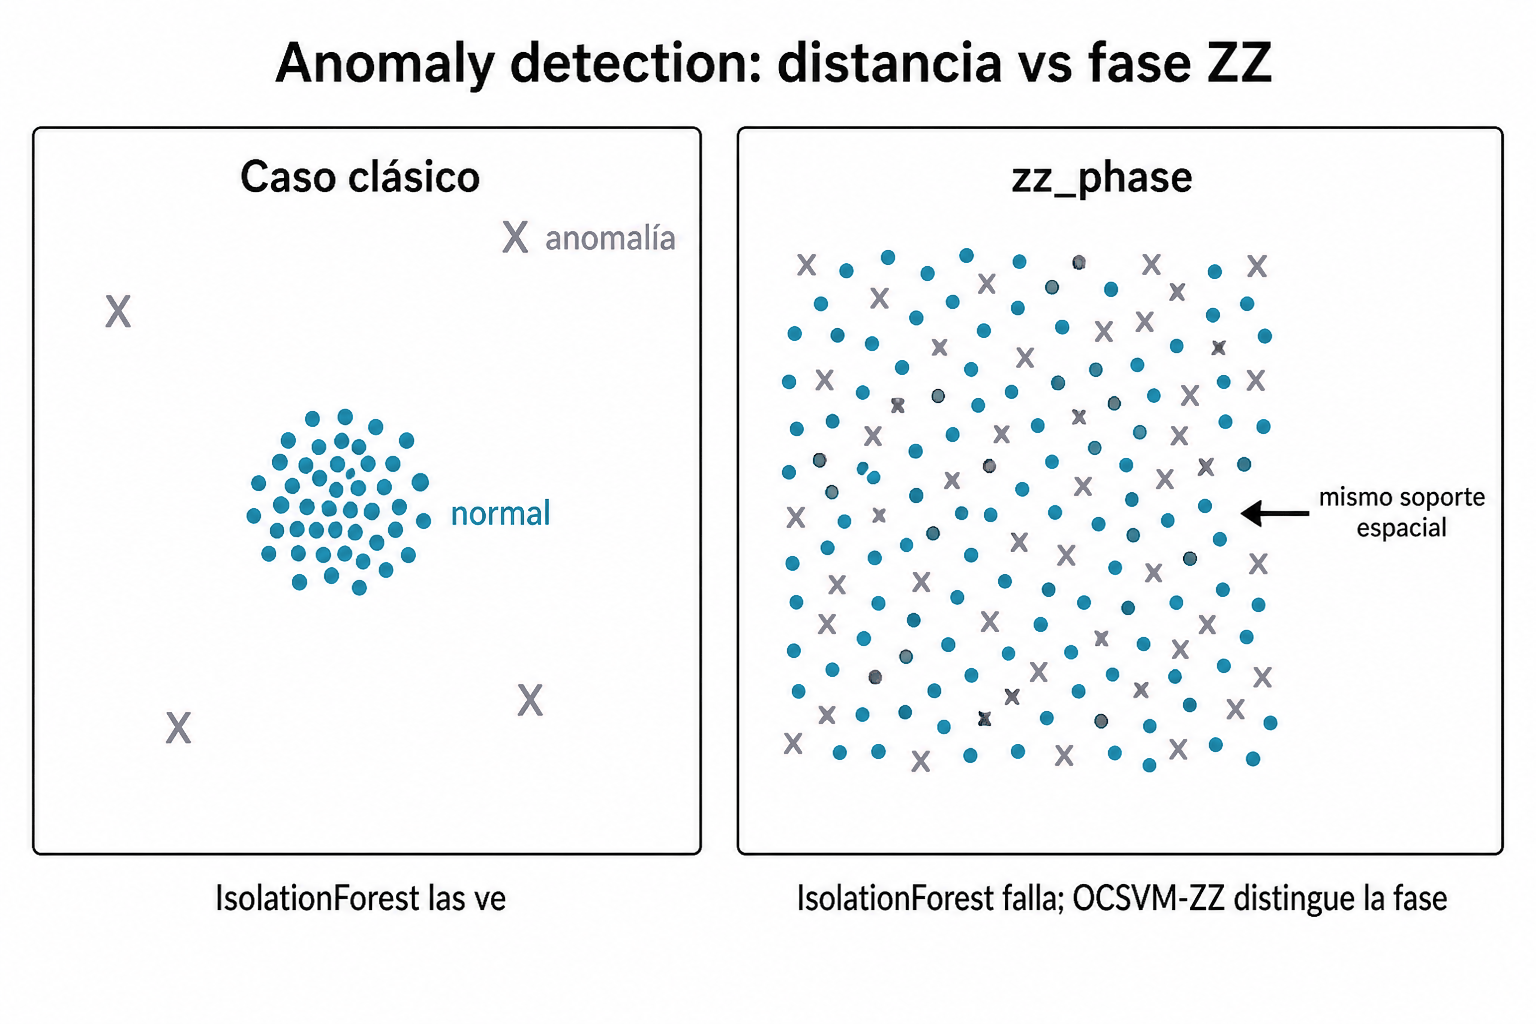
\includegraphics[width=0.98\textwidth]{Imagenes/zz_phase_concept_diagram.png}
\caption{Idea geométrica del Caso~8. Izquierda: anomalía por distancia (IsolationForest la detecta). Derecha: anomalía por estructura de fase alineada al feature map, mismo soporte espacial (IsolationForest falla; OCSVM-ZZ puede separar ---mapa validado: ZZ).}
\label{fig:anomaly_concept}
\end{figure}

\begin{figure}[!htbp]
\centering
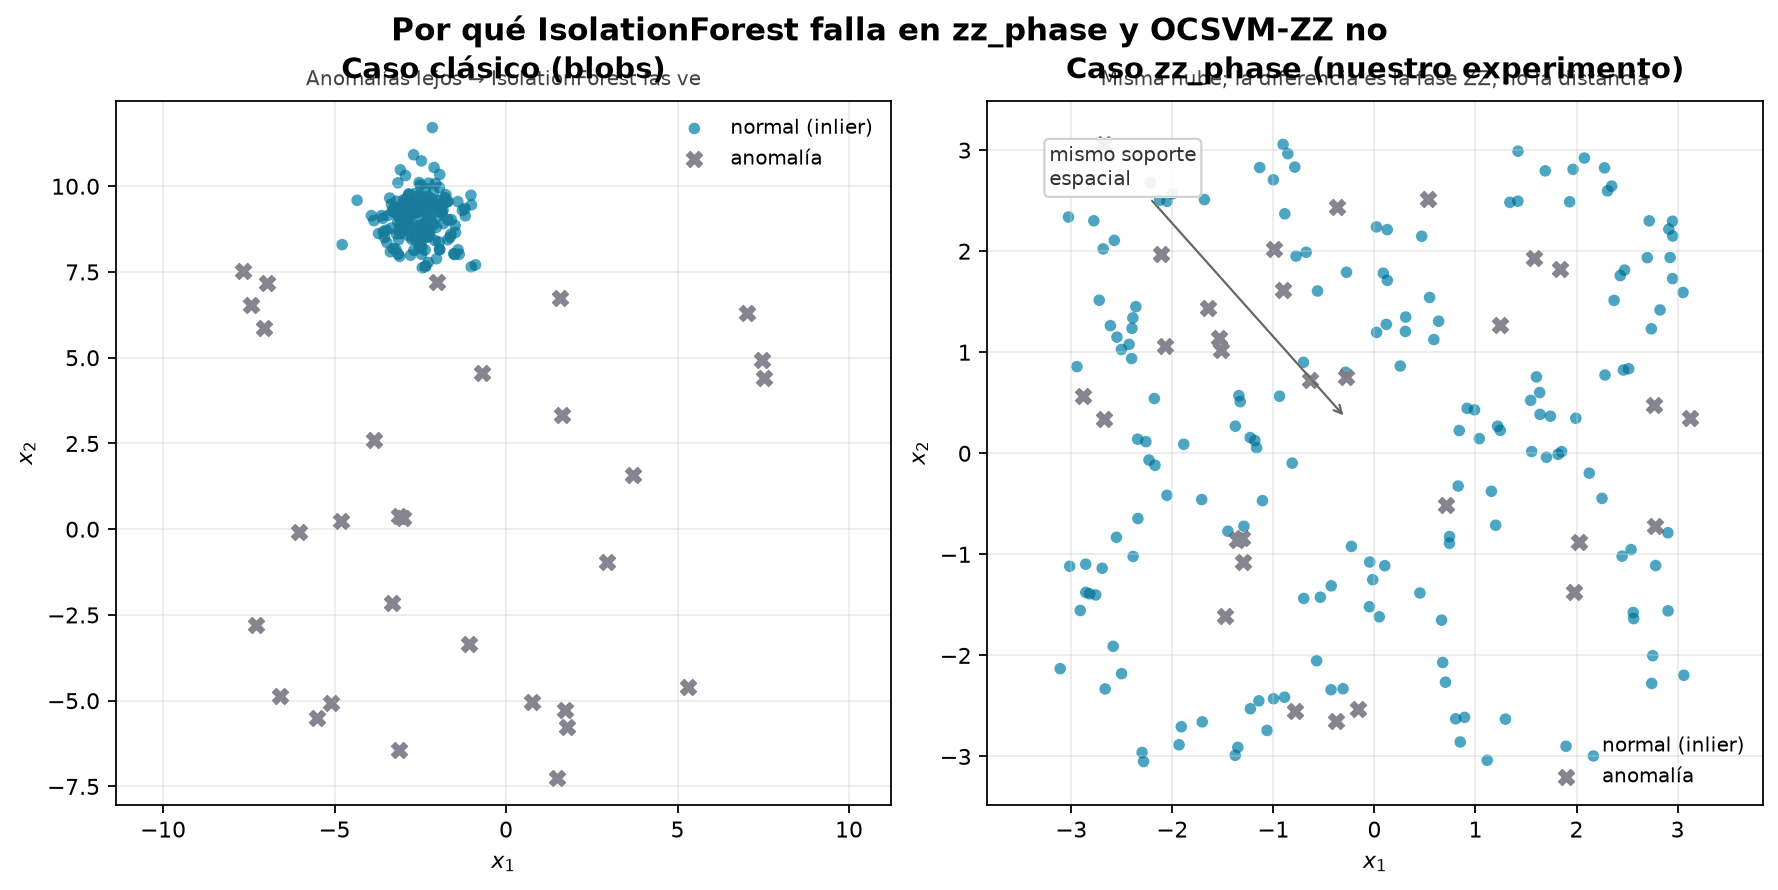
\includegraphics[width=0.98\textwidth]{Imagenes/zz_phase_vs_blobs_anomaly.png}
\caption{Datos reales del generador QML~v2. En \texttt{blobs} las anomalías están lejos del blob de inliers; en \texttt{zz\_phase} normales y anomalías comparten la misma nube en el plano de ángulos.}
\label{fig:anomaly_support}
\end{figure}

% =====================================================================
\section{Caso de uso 9: Forecasting one-step por lags (QK-SVR)}
\label{sec:caso9_timeseries}
% =====================================================================

Este caso extiende la familia de kernels a \textbf{series temporales} con un protocolo justo de predicción un paso adelante: $y_t$ se estima únicamente a partir de una ventana de los valores anteriores (\textit{lags}). No es una comparación frente a ARIMA o Prophet: la pregunta es si un kernel ZZ sobre el vector de lags supera a regresores clásicos que ven \emph{los mismos lags}. Implementación: \texttt{POCs/qml\_v2/timeseries.py}; cuaderno: Notebook~12.

\subsection{Protocolo}

\begin{itemize}
  \item \textbf{Tabla~A:} QK-SVR (kernel de fidelidad ZZ, $n_q=2$ qubits), Ridge, SVR-RBF y Gradient Boosting reciben las mismas $n_{\mathrm{lags}}=n_q=2$ variables.
  \item \textbf{Tabla~B:} los clásicos reciben además 4 lags adicionales, media y desviación de la ventana y, en la serie SKG, la hora del día en codificación cíclica (mismas muestras de entrenamiento).
  \item \textbf{División temporal:} el 70\,\% inicial de la serie es entrenamiento y el 30\,\% final es prueba, sin barajar, de modo que no hay fuga de información del futuro. 5 repeticiones.
  \item \textbf{Referencias ingenuas:} el MAE de la \emph{persistencia} ($\hat y_t=y_{t-1}$) y el de predecir la media del entrenamiento sobre las mismas ventanas de prueba, para interpretar el error absoluto de cada modelo.
\end{itemize}

\subsection{Datasets e hipótesis}

La Figura~\ref{fig:ts_datasets} muestra los tres conjuntos.

\begin{itemize}
  \item \texttt{zz\_lag} (cuántico-nativo): pares de lags $(y_{t-2},y_{t-1})$ en $[-\pi,\pi]^2$ y objetivo $y_t=\langle ZZ\rangle$ del estado preparado por el mapa ZZ con esos ángulos, de modo que target y feature map están alineados por construcción. Los pares son independientes entre sí: es el control nativo del protocolo, no una serie con dinámica propia. Cada repetición toma 160 ventanas de un conjunto de 320.
  \item \texttt{sine} (referencia sintética): $\sin(2\pi t/24)+0.3\sin(2\pi t/7)$ más ruido gaussiano ($\sigma=0.15$), 480 puntos; cada repetición toma una ventana contigua de 160. Periodicidad clásica.
  \item \texttt{skg\_speed} (SKG, datos de práctica): velocidad de los corredores viales de Bogotá (\texttt{bctraveltimes\_history.csv}; 582 corredores con una lectura cada 5 minutos durante 12~h). Cada repetición usa un corredor distinto (los 5 con más lecturas, 144 cada uno, 138 ventanas), de forma que las repeticiones no reutilizan la misma serie.
\end{itemize}

\begin{figure}[ht]
\centering
\includegraphics[width=\textwidth]{../POCs/data/output/figures/12_series_datasets.png}
\caption{Datasets del Caso~9. Izquierda: \texttt{zz\_lag}, con los dos lags como ejes y el objetivo $\langle ZZ\rangle$ como color. Centro y derecha: \texttt{sine} y un corredor de \texttt{skg\_speed}, con la zona de prueba (futuro) sombreada. Fuente: Notebook~12.}
\label{fig:ts_datasets}
\end{figure}

\subsection{Resultados (Tabla~A)}

\begin{table}[ht]
\centering
\small
\begin{tabular}{llcc}
\hline
\textbf{Dataset} & \textbf{Mejor Tabla~A} & \textbf{MAE} & \textbf{Lectura} \\
\hline
\texttt{zz\_lag} & \textbf{QK-SVR-ZZ} & \textbf{0.056} frente a Ridge 0.414 & Target $=\langle ZZ\rangle$ \\
\texttt{sine} & SVR-RBF & 0.260 frente a QK-SVR 0.662 & Periodicidad clásica \\
\texttt{skg\_speed} & Ridge & 2.80 frente a QK-SVR 13.59 & Práctica; clásico \\
\hline
\end{tabular}
\caption{Caso~9. MAE en test (media de 5 repeticiones). Ventaja solo cuando el generador del target está alineado con el feature map (aquí ZZ en \texttt{zz\_lag}). Fuente: \texttt{fair\_timeseries\_*.csv}.}
\label{tab:timeseries_dev}
\end{table}

\paragraph{Lectura.}
Mismo principio transversal que en clasificación y anomalías: no ``ZZ gana en series'', sino ``el mapa alineado gana; ZZ es el que medimos''. Fuera del régimen nativo el kernel ZZ de 2 qubits no extrae señal: su MAE coincide con el de predecir la media del entrenamiento ($0.662$ frente a $0.658$ en \texttt{sine}; $13.59$ frente a $13.61$ en \texttt{skg\_speed}), mientras que Ridge se sitúa en el nivel de la persistencia ($2.80$ frente a $2.75$ en SKG). En el corredor SKG la opción operativa es, por tanto, un modelo lineal sobre lags (o la propia persistencia); añadir variables clásicas (Tabla~B) no mejora el resultado con series de solo 138 ventanas.

% =====================================================================
\section{Prototipo de arquitectura híbrida cuántico-clásica}
\label{sec:prototipo_hibrido}
% =====================================================================

Los nueve casos de uso desarrollados en este capítulo ilustran, cada uno desde un ángulo diferente, la misma idea estructural: los algoritmos cuánticos variacionales de la era NISQ no reemplazan a los clásicos sino que se integran con ellos en un \textbf{pipeline híbrido} donde cada parte hace lo que mejor sabe hacer. Esta sección sintetiza ese patrón de diseño en forma de prototipo arquitectónico aplicable a un entorno empresarial como SKG Tecnología.

\subsection{Principio de diseño: separación de responsabilidades}

La arquitectura híbrida cuántico-clásica se sustenta en una premisa simple: el módulo cuántico resuelve la parte del problema que es difícil para los computadores clásicos —la exploración de espacios de búsqueda exponencialmente grandes o la evaluación de kernels en espacios de Hilbert de alta dimensión—, mientras que el módulo clásico orquesta el flujo, pre-procesa los datos, ejecuta la optimización de parámetros y toma la decisión final a partir de los resultados cuánticos.

\subsection{Flujo de decisión: cuándo activar el módulo cuántico}

No todos los problemas se benefician del módulo cuántico. La Tabla~\ref{tab:flujo_hibrido} resume el criterio de activación según el tipo de problema.

\begin{table}[ht]
\centering
\small
\begin{tabular}{>{\raggedright\arraybackslash}p{3.2cm}>{\raggedright\arraybackslash}p{3.2cm}>{\raggedright\arraybackslash}p{3.5cm}>{\raggedright\arraybackslash}p{3.0cm}}
\hline
\textbf{Tipo de problema} & \textbf{Criterio de activación} & \textbf{Módulo cuántico} & \textbf{Módulo clásico} \\
\hline
Clasificación / Regresión &
$\mathcal{Q}(\mathcal{D}) > 0$ (score de cuanticidad positivo) &
QSVM / QK-SVR (kernel cuántico) &
Gradient Boosting como fallback \\
\hline
Detección de anomalías (one-class) &
Anomalía alineada al feature map (p.\,ej.\ \texttt{zz\_phase}, $\mathcal{Q}>0$) &
OCSVM-ZZ (u otro kernel si el mapa cambia) &
IsolationForest / LOF como default \\
\hline
Forecasting (lags) &
Target alineado al mapa (p.\,ej.\ \texttt{zz\_lag}) &
QK-SVR (ZZ u otro) &
Ridge / SVR-RBF / GB \\
\hline
Optimización combinatoria / TSP &
QUBO factible; $n_{\text{vars}}$ compatible con hardware &
QAOA ($p \geq 1$) &
NN+2-opt / ILP / verificación \\
\hline
Caso general &
$\mathcal{Q}(\mathcal{D}) \leq 0$ o $n_{\text{vars}} > 50$ &
No se activa &
Pipeline clásico estándar \\
\hline
\end{tabular}
\caption{Criterio de activación del módulo cuántico en la arquitectura híbrida propuesta.}
\label{tab:flujo_hibrido}
\end{table}

\subsection{Arquitectura de referencia}

El prototipo conceptual se articula en cuatro capas:

\begin{enumerate}
  \item \textbf{Capa de diagnóstico} (\textit{clásica}): Calcula el score $\mathcal{Q}(\mathcal{D})$ o verifica si el problema es formulable como QUBO. Decide si el módulo cuántico es pertinente. Esta capa emplea exclusivamente computación clásica y tiene coste lineal en el tamaño del dataset.

  \item \textbf{Capa de preprocesamiento} (\textit{clásica}): Aplica, si es necesario, el Framework QCR (re-uploading, rotación, reducción dimensional) para maximizar la compatibilidad cuántica de los datos. Para problemas de optimización, construye la matriz QUBO y la traduce a \texttt{SparsePauliOp}.

  \item \textbf{Capa de cómputo cuántico} (\textit{cuántica}): Ejecuta el circuito cuántico — kernel cuántico (para clasificación/regresión) o QAOA/VQE (para optimización) — sobre el simulador Aer o sobre hardware IBM Quantum. Devuelve la energía esperada (optimización) o los valores del kernel (clasificación).

  \item \textbf{Capa de decisión} (\textit{clásica}): Integra el resultado cuántico en el pipeline existente: el optimizador COBYLA actualiza los parámetros del circuito (loop híbrido), o el clasificador SVM toma la predicción final a partir de la matriz de kernel cuántico. El resultado final es siempre una salida clásica (asignación, etiqueta, regresión).
\end{enumerate}

\begin{figure}[!htbp]
\centering
\begin{tikzpicture}[thick, font=\small,
    capa/.style={rectangle, rounded corners=5pt, very thick,
                 minimum width=0.92\textwidth, text width=0.88\textwidth,
                 align=center, inner sep=7pt},
    arr/.style={->, very thick}]

  % --- Capa 1: Diagnóstico ---
  \node[capa, draw=gray!60!black, fill=gray!10] (c1) {
    \textbf{Capa 1 — Diagnóstico} \normalfont\footnotesize(clásica)\\[3pt]
    {\scriptsize\color{gray!55!black}%
     Calcula $\mathcal{Q}(\mathcal{D})$ / verifica formulación QUBO
     \;$\rightarrow$\; \textquestiondown{}activar módulo cuántico?}
  };

  % --- Capa 2: Preprocesamiento ---
  \node[capa, draw=orange!55!black, fill=orange!7, below=0.5cm of c1] (c2) {
    \textbf{Capa 2 — Preprocesamiento} \normalfont\footnotesize(clásica)\\[3pt]
    {\scriptsize\color{orange!65!black}%
     Framework QCR: re-uploading / rotación / QUBO $\rightarrow$ \texttt{SparsePauliOp}}
  };

  % --- Capa 3: Cómputo cuántico ---
  \node[capa, draw=blue!55!black, fill=blue!7, below=0.5cm of c2] (c3) {
    \textbf{Capa 3 — Cómputo cuántico} \normalfont\footnotesize(cuántica)\\[3pt]
    {\scriptsize\color{blue!65!black}%
     Kernel cuántico (QSVM) \;$|$\; QAOA/VQE \quad Aer / IBM Quantum Hardware}
  };

  % --- Capa 4: Decisión ---
  \node[capa, draw=teal!55!black, fill=teal!7, below=0.5cm of c3] (c4) {
    \textbf{Capa 4 — Decisión} \normalfont\footnotesize(clásica)\\[3pt]
    {\scriptsize\color{teal!65!black}%
     SVM / COBYLA actualiza $\boldsymbol{\theta}$
     \;$\rightarrow$\; salida: etiqueta / asignación / regresión}
  };

  % --- Flechas ---
  \draw[arr] (c1.south) -- node[right=5pt, font=\scriptsize]{Sí: continuar} (c2.north);
  \draw[arr] (c2.south) -- (c3.north);
  \draw[arr] (c3.south) -- (c4.north);
  \draw[arr] (c4.south) -- ++(0,-0.55)
    node[below, font=\scriptsize]{Resultado clásico final};

\end{tikzpicture}
\caption{Arquitectura de referencia del prototipo híbrido en cuatro capas. Las capas 1, 2 y 4 son puramente clásicas; la capa 3 es el único punto de ejecución cuántica. Esta separación permite desactivar el módulo cuántico sin modificar el resto del pipeline.}
\label{fig:arquitectura_cuatro_capas}
\end{figure}

\subsection{Posicionamiento como herramienta complementaria}

Una reflexión importante que emerge del análisis experimental es que la arquitectura híbrida no tiene sentido como sistema aislado, sino como \textbf{herramienta adicional dentro del stack tecnológico existente}. En el caso de SKG Tecnología, el sistema actual de gestión de incidentes y asignación de recursos seguiría operando con sus algoritmos clásicos consolidados. El módulo cuántico solo se activaría en los subproblemas donde se demuestre una ventaja medible. En los experimentos de este trabajo eso se cumple de forma condicional en clasificación con estructura cuántica (Caso~1) y no se cumple en optimización combinatoria de asignación de recursos, donde la formulación QUBO es natural y el QAOA con $p=1$ recupera el óptimo, pero empata con los métodos exactos (Caso~3).

La adopción de esta arquitectura no requiere reemplazar ningún sistema existente, sino añadir un módulo con interfaz bien definida ---$2p$ parámetros de entrada, 1 escalar de salida--- que puede ser desactivado sin consecuencias si el hardware cuántico no está disponible o si el problema no cumple los criterios de activación de la Tabla~\ref{tab:flujo_hibrido}.

% !TEX root = ../main.tex
\chapter{Resultados y análisis}\label{cap:evaluacion}

Este capítulo presenta el análisis cuantitativo y cualitativo de los resultados obtenidos en cada caso de uso, discute las diferencias de rendimiento entre algoritmos cuánticos y clásicos a la luz del estado del arte, y evalúa las implicaciones prácticas para su aplicación en el contexto operativo de SKG Tecnología. Para cada caso se identifican explícitamente las condiciones bajo las que se observa ventaja cuántica, las limitaciones que explican los resultados negativos, y las perspectivas de mejora a medida que el hardware cuántico avance.

% =====================================================================
\section{Caso de uso 1: Clasificación supervisada}
% =====================================================================

\subsection{Dataset cuántico-nativo: ventaja por construcción}

Los resultados sobre el dataset con estructura cuántica explícita constituyen la evidencia empírica más clara del estudio, aunque obtenida sobre datos alineados con el kernel por construcción. El QSVM alcanzó una exactitud del \textbf{91.7\%}, frente al 53.3\% del mejor clasificador clásico (SVM polinomial de grado 3; SVM-RBF: 46.7\%, Gradient Boosting: 51.7\%, SVM lineal: 45.0\%), lo que supone una \textbf{ventaja de +38.3 puntos porcentuales (pp)}. Este resultado es el esperado por construcción, y coherente con la idea de \cite{liu2021} y \cite{huang2021} de que la ventaja exige un kernel alineado con las etiquetas: cuando estas se definen mediante una función cuántica, el kernel cuántico las aprende con alta precisión mientras que los clasificadores clásicos probados (RBF, polinomial, lineal y Gradient Boosting) quedan cerca del azar.

El análisis de escalabilidad (Tabla~\ref{tab:escala_clasificacion}) repite el experimento 10 veces por tamaño (\texttt{python -m qml\_v2.scalability}): en cada repetición se regenera el dataset con una semilla distinta, se reserva el 30\% como test y se entrena con los primeros $n$ ejemplos. La ventaja del QSVM sobre el mejor clásico (SVM-RBF o Gradient Boosting) es positiva en las 10 repeticiones de los seis tamaños $n \in [30, 180]$, con una media de \textbf{+33.2 pp} (de $+27.1$~pp para $n=30$ a $+37.6$~pp para $n=180$) y un intervalo de confianza del 95\% que no incluye el cero en ningún tamaño (límite inferior mínimo: $+22.1$~pp). La exactitud del QSVM crece con $n$ ($79.6\%$ a $92.6\%$), mientras que los clásicos permanecen cerca del azar. La partición única del Notebook~01 (media $+40.9$~pp, máximo $+48.9$~pp para $n=50$) cae por encima de este rango y debe leerse como una realización optimista.

\begin{table}[ht]
\centering
\small
\resizebox{\textwidth}{!}{%
\begin{tabular}{rccccc}
\hline
$n$ & QSVM (\%) & SVM-RBF (\%) & Grad.\ Boosting (\%) & $\Delta$ vs.\ mejor clásico (pp) [IC 95\%] & Rep.\ con ventaja \\
\hline
30 & $79.6\pm5.9$ & $51.0\pm4.9$ & $49.0\pm5.2$ & $+27.1$ [$+22.1$, $+32.2$] & 10/10 \\
50 & $87.1\pm5.1$ & $49.9\pm4.2$ & $53.1\pm5.6$ & $+32.9$ [$+27.7$, $+38.1$] & 10/10 \\
80 & $88.4\pm2.5$ & $48.6\pm5.8$ & $55.0\pm6.2$ & $+32.9$ [$+27.9$, $+37.9$] & 10/10 \\
100 & $89.6\pm4.2$ & $48.7\pm4.8$ & $55.8\pm7.5$ & $+33.8$ [$+27.3$, $+40.2$] & 10/10 \\
140 & $90.0\pm3.1$ & $50.9\pm3.9$ & $54.7\pm4.3$ & $+35.1$ [$+32.2$, $+38.0$] & 10/10 \\
180 & $92.6\pm2.6$ & $49.0\pm3.6$ & $55.0\pm6.2$ & $+37.6$ [$+33.4$, $+41.7$] & 10/10 \\
\hline
\end{tabular}}
\caption{Escalabilidad de la ventaja cuántica en clasificación (dataset cuántico-nativo, ZZFeatureMap de 2 qubits): media $\pm$ desviación sobre 10 repeticiones y 90 ejemplos de test por repetición. El $\Delta$ se calcula en cada repetición frente al mejor de los dos clásicos; el IC es de 95\% (t de Student). Fuente: \texttt{fair\_scalability\_native.csv}.}
\label{tab:escala_clasificacion}
\end{table}

\begin{figure}[ht]
\centering
\includegraphics[width=0.92\textwidth]{../POCs/data/output/figures/01_escalabilidad_ventaja_clasificacion.png}
\caption{Escalabilidad de la ventaja cuántica en el dataset cuántico-nativo según el tamaño del conjunto de entrenamiento ($n \in [30, 180]$; 10 repeticiones por tamaño). Izquierda: exactitud media $\pm$ desviación de QSVM, SVM-RBF y Gradient Boosting. Derecha: ventaja del QSVM sobre el mejor clásico con su intervalo de confianza del 95\%; entre paréntesis, repeticiones con ventaja. Los datasets reales (SKG, Telco) no se evaluaron en esta curva. Fuente: \texttt{fair\_scalability\_native.csv}.}
\label{fig:escala_clasificacion}
\end{figure}

El mecanismo que explica esta ventaja es la \textbf{alineación} entre el feature map y el generador de etiquetas: en este experimento ambas son el mismo \texttt{ZZFeatureMap} (mapa empíricamente validado en el TFM), de modo que el kernel minimiza el riesgo empírico en el \textbf{espacio de representación} correcto ---el espacio de Hilbert $\mathcal{H}$ inducido por $\phi\colon\mathbb{R}^2\rightarrow\mathcal{H}$---. La lección no es ``ZZ gana'', sino ``el mapa alineado gana''. Los clasificadores clásicos operan en $\mathbb{R}^2$ y no acceden a ese espacio de Hilbert sin coste exponencial.

\paragraph{Limitaciones que condicionan la interpretación.}
\begin{itemize}
  \item El dataset es artificial: está diseñado a medida para el kernel cuántico. La ventaja observada es una cota superior del rendimiento cuántico en condiciones ideales.
  \item La simulación exacta sin ruido es optimista respecto al hardware NISQ real; la decoherencia reduciría la fidelidad del kernel y, por tanto, la ventaja.
  \item El kernel exige $O(n^2)$ evaluaciones de fidelidad; con 2 qubits la simulación exacta es inmediata, pero en hardware, con la fidelidad estimada por muestreo y más qubits, ese coste limita la escala.
\end{itemize}

\begin{figure}[ht]
\centering
\includegraphics[width=0.95\textwidth]{../POCs/data/output/figures/06_quantum_kernel_boundaries.png}
\caption{Fronteras de decisión de SVM-RBF (izquierda), Gradient Boosting (centro) y QSVM (derecha) sobre el dataset cuántico-nativo en 2D. El QSVM genera una frontera curvada y más compleja (exactitud 93.3\%); el SVM-RBF, una frontera más suave (53.3\%), y el Gradient Boosting, una frontera por rectángulos (73.3\%). El test tiene solo 15 puntos (cada acierto equivale a 6.7~pp) y la frontera del QSVM se estima sobre una malla de $12\times12$, por lo que la figura es ilustrativa y no una medida de rendimiento; la evidencia cuantitativa es la del Caso~1.}
\label{fig:kernel_boundaries}
\end{figure}

\subsection{Dataset SKG Tecnología: resultado esperado en era NISQ}

Sobre el dataset real de incidentes de movilidad de Bogotá, el QSVM obtuvo exactitud del \textbf{55.0\%}, inferior al \textbf{59.5\%} del mejor clasificador clásico (SVM-RBF): \textbf{desventaja de $-$4.5 pp}. Este resultado es el esperado en la era NISQ con datos reales: los incidentes de movilidad no presentan la estructura cuántica que el kernel explota.

Cabe destacar que ningún modelo ---cuántico ni clásico--- superó el 80\% de exactitud sobre este dataset, lo que indica que la limitación no es del algoritmo sino de las features disponibles. La reducción a 2 dimensiones mediante PCA (varianza explicada: 84.6\%) implica una pérdida del 15.4\% de la información discriminativa. Un kernel cuántico de 4--6 qubits podría operar sobre más features sin esta pérdida, acortando potencialmente la brecha.

\paragraph{Implicaciones para SKG.}
La pequeña brecha de rendimiento ($-$4.5 pp) sugiere que el QSVM no es inferior en un orden de magnitud a los clásicos en este dominio, lo que lo convierte en un candidato técnicamente viable para evaluación en hardware cuántico real de generaciones futuras con mayor número de qubits lógicos.

\subsection{Dataset Telco Churn: caso control validado}

Sobre el dataset de referencia, el QSVM obtuvo un \textbf{76.0\%} de exactitud frente al \textbf{79.8\%} del Gradient Boosting: \textbf{desventaja de $-$3.8 pp}. Esta comparación del Notebook~01 es \textbf{asimétrica}, y conviene leerla como una cota optimista para el QSVM: los clasificadores clásicos usan las 21 variables, 5\,634 ejemplos de entrenamiento y los 1\,409 de test, mientras que el QSVM usa 4 componentes PCA (48.5\% de la varianza), 100 ejemplos de entrenamiento y solo 50 de test, de modo que cada acierto equivale a 2 pp. Por eso la cifra de $-3.8$~pp no es una medida homogénea de la brecha.

El protocolo justo de \texttt{qml\_v2} (Tabla~\ref{tab:clasif_justa}) corrige esa asimetría: mismas particiones, mismo número de ejemplos y, en la tabla~A, las mismas variables para todos los modelos, con 10 repeticiones. En Telco el QSVM queda en $53.3\pm9.3\%$ frente al $77.2\pm4.3\%$ de la regresión logística ($-23.8$~pp), y a $26.2$~pp del Gradient Boosting con todas las variables. Esto confirma, con mayor margen, que en ausencia de estructura cuántica los clasificadores clásicos son superiores: el QSVM no gana por defecto, sino solo cuando existe la alineación entre mapa y datos que la teoría sugiere.

\begin{table}[ht]
\centering
\footnotesize
\setlength{\tabcolsep}{4pt}
\resizebox{\textwidth}{!}{%
\begin{tabular}{lccccc}
\toprule
\textbf{Dataset} & \textbf{QSVM-ZZ} & \textbf{Mejor clásico (A)} & \textbf{$\Delta$ (A)} & \textbf{Mejor clásico (B)} & \textbf{$\Delta$ (B)} \\
\midrule
Cuántico-nativo & $88.8\pm5.8$ & GB $52.3\pm6.0$ & $+36.5$ & --- & --- \\
SKG Incidentes & $49.5\pm7.0$ & GB $52.7\pm5.7$ & $-3.2$ & SVM lineal (7 var.) $56.2\pm5.3$ & $-6.7$ \\
Telco Churn & $53.3\pm9.3$ & Reg. logística $77.2\pm4.3$ & $-23.8$ & GB (19 var.) $79.5\pm2.9$ & $-26.2$ \\
\bottomrule
\end{tabular}}
\caption{Protocolo justo de clasificación (\texttt{qml\_v2.classification}); GB = Gradient Boosting. Exactitud en test (\%, media $\pm$ desviación sobre 10 repeticiones; 140 ejemplos de entrenamiento y 60 de test). A: todos los modelos con las mismas 2 variables que el QSVM. B: clásicos con todas las variables originales. $\Delta$ en puntos porcentuales respecto al QSVM. Fuente: \texttt{fair\_classification\_all.csv}.}
\label{tab:clasif_justa}
\end{table}

\begin{figure}[!htbp]
\centering
\includegraphics[width=0.95\textwidth]{../POCs/data/output/figures/01_clasificacion_comparacion.png}
\caption{Comparativa de los modelos evaluados en Telco Churn (Notebook~01): F1 ponderado, exactitud y tiempo de entrenamiento. Los modelos clásicos usan las 21 variables y la partición completa; el QSVM y el VQC, 4 componentes PCA y 100/50 ejemplos de entrenamiento/test (comparación asimétrica; véase la Tabla~\ref{tab:clasif_justa}).}
\label{fig:clasificacion_comparacion}
\end{figure}

\begin{figure}[!htbp]
\centering
\includegraphics[width=\textwidth]{../POCs/data/output/figures/06_learning_curves_quantum_advantage.png}
\caption{Curvas de aprendizaje del QSVM y del SVM-RBF en función del tamaño de entrenamiento $n \in [30, 180]$, sobre el dataset cuántico-nativo del Caso~1 (media de 10 repeticiones; la banda es $\pm$ una desviación típica; derecha: ventaja media sobre el SVM-RBF en puntos porcentuales). La brecha es positiva en todo el rango evaluado y no se cierra al aumentar $n$. Fuente: \texttt{fair\_scalability\_native.csv}.}
\label{fig:learning_curves}
\end{figure}

% =====================================================================
\section{Caso de uso 2: Regresión con kernel cuántico}
% =====================================================================

Los resultados de regresión son mayoritariamente negativos para el kernel cuántico: solo el dataset construido con el propio mapa de características muestra una diferencia a su favor, que es por construcción. La Tabla~\ref{tab:regresion_3ds} resume los resultados del Notebook~03 (una partición) y la Tabla~\ref{tab:regresion_justa}, los del protocolo justo de \texttt{qml\_v2} (10 repeticiones, mismas particiones y variables).

\begin{table}[ht]
\centering
\resizebox{\textwidth}{!}{%
\begin{tabular}{lcccc}
\hline
\textbf{Dataset} & \textbf{QK-SVR ($R^2$)} & \textbf{Mejor clásico ($R^2$)} & \textbf{$\Delta R^2$} & \textbf{Resultado} \\
\hline
Cuántico-nativo  & $+0.985$  & $+0.020$ (SVR-Poly)  & $\mathbf{+0.965}$ & \textbf{Ventaja (por construcción)} \\
SKG Corredores   & $+0.098$  & $+0.660$ (GradBoost) & $-0.562$ & Desventaja \\
Friedman \#1     & $-0.151$  & $+0.777$ (XGBoost)   & $-0.928$ & Desventaja \\
\hline
\end{tabular}}
\caption{Comparativa de regresión cuántica vs clásica en los tres datasets. El mejor clásico incluye XGBoost, Random Forest, SVR-RBF y Ridge.}
\label{tab:regresion_3ds}
\end{table}

\subsection{Dataset cuántico-nativo: ventaja por construcción}

El dataset cuántico-nativo de regresión se genera con $y(\mathbf{x})=\langle ZZ\rangle$ evaluado sobre el estado preparado por el propio \texttt{ZZFeatureMap} (2 qubits, 200 muestras, $\mathbf{x}\in[-\pi,\pi]^2$). El QK-SVR obtuvo $R^2=0.985$ frente a $R^2=0.020$ del mejor clásico (SVR-Poly), una diferencia de $\Delta R^2=+0.965$: el kernel cuántico reproduce casi exactamente la función objetivo porque esta es lineal en su espacio de características, mientras que ninguno de los modelos clásicos supera el nivel de una predicción constante ($R^2\approx0$). El protocolo justo confirma el resultado con 10 repeticiones ($R^2=0.986\pm0.002$ frente a $-0.016\pm0.139$ de Random Forest; $\Delta R^2=+1.002$). Como en clasificación, esta ventaja es \textbf{por construcción}: el objetivo se genera con el mismo mapa que usa el kernel, y no demuestra ventaja sobre datos reales.

\paragraph{Limitaciones.}
\begin{itemize}
  \item Los hiperparámetros no se ajustan de forma homogénea entre datasets en el Notebook~03. En el dataset nativo, el QK-SVR usa $C=10$, $\varepsilon=0.1$ y los SVR clásicos sus valores por defecto ($C=1$). En Friedman~\#1, $C$ y $\varepsilon$ del QK-SVR se eligen en una malla de 9 combinaciones ($C\in\{10,50,100\}$, $\varepsilon\in\{0.5,1,2\}$) maximizando el $R^2$ \emph{sobre el propio conjunto de test}, lo que favorece al modelo cuántico (y aun así pierde); los clásicos usan sus valores por defecto. En SKG, el QK-SVR usa $C=10$, $\varepsilon=0.05$ con el objetivo reescalado a $[0,1]$ y el SVR-RBF clásico $C=10$, $\varepsilon=0.5$. En el protocolo justo todos los SVR usan $C=10$, $\varepsilon=0.1$, por lo que una búsqueda más amplia sobre $C$ y $\varepsilon$ podría modificar el $R^2$ de los clásicos.
  \item El Notebook~03 usa una única partición (140 entrenamientos, 60 de test) y no ofrece intervalo de confianza; la repetición del protocolo justo sí lo hace (desviación $0.002$ del QK-SVR).
\end{itemize}

\subsection{Dataset SKG Tecnología: limitaciones estructurales}

El QK-SVR obtuvo $R^2 = 0.098$ (RMSE = 11.04 km/h) frente al $R^2 = 0.660$ del Gradient Boosting (RMSE = 7.25 km/h): \textbf{desventaja de $\Delta R^2 = -0.562$}. La magnitud de esta brecha se explica por tres factores concurrentes:

\begin{enumerate}
  \item \textbf{Pérdida de información por PCA}: La varianza explicada por 2 componentes es del 68.6\%, lo que significa que el 31.4\% de la varianza de las features originales ---incluyendo patrones temporales y de nivel de servicio--- no está disponible para el QK-SVR.
  \item \textbf{Desperdicio de datos}: El QK-SVR se entrena con 150 observaciones frente a las 64\,896 (80\% de 81\,121) de los clásicos, es decir, el 0.23\% de sus datos de entrenamiento. Esta asimetría hace la comparación inherentemente desigual.
  \item \textbf{Estructura del problema}: La correlación entre \texttt{levelofservice} y \texttt{speed} es cuasi-determinista en los datos de SKG (verde $\approx$ rápido, rojo $\approx$ lento), una relación que los árboles de decisión capturan con una sola partición, sin necesidad de un kernel cuántico.
\end{enumerate}

\subsection{Dataset Friedman \#1: ventaja clásica}

Sobre el benchmark sintético Friedman~\#1 \citep{friedman1991}, con $y=10\sin(\pi x_1x_2)+20(x_3-0.5)^2+10x_4+5x_5+\varepsilon$, el QK-SVR obtuvo $R^2=-0.151$ frente a $R^2=0.777$ de XGBoost (también superan al kernel cuántico la regresión lineal, $0.641$, y Random Forest, $0.704$): $\Delta R^2=-0.928$. Aunque el término $\sin(\pi x_1x_2)$ recuerda a la interacción $x_ix_j$ codificada por las puertas $ZZ$, el kernel cuántico, con 5 qubits (uno por variable) en el Notebook~03 y con 2 componentes PCA en el protocolo justo, no lo aprovecha. Friedman~\#1 no es un problema de ventaja cuántica: es una referencia clásica en la que los métodos de árboles dominan.

\subsection{Protocolo justo de regresión}

Como en el Caso~1, las comparaciones del Notebook~03 no son homogéneas, aunque la asimetría es distinta en cada dataset. En \textbf{Friedman~\#1} (300 muestras: 210 de entrenamiento y 90 de test) el QK-SVR usa las 5 variables (5 qubits) pero solo 150 de las 210 muestras de entrenamiento y las primeras 60 de test; los clásicos se entrenan con las 210, aunque en la tabla se evalúan sobre esas mismas 60 muestras de test. La ventaja clásica no se explica por falta de variables, solo en parte por los 60 ejemplos de entrenamiento adicionales. En \textbf{SKG} la asimetría es mucho mayor: el QK-SVR usa 2 componentes PCA de 4 variables (68.6\% de la varianza), 150 muestras de entrenamiento y 80 de test, mientras que los clásicos usan las 4 variables, 64\,896 muestras de entrenamiento y 16\,225 de test, de modo que sus $R^2$ no están medidos sobre los mismos puntos. El protocolo \texttt{qml\_v2.regression} las homogeneiza (Tabla~\ref{tab:regresion_justa}): mismas particiones (140/60), 10 repeticiones y, en la tabla~A, las mismas variables para todos los modelos. El patrón se mantiene y se acentúa: el QK-SVR gana solo en el dataset nativo ($\Delta R^2=+1.002$) y pierde en SKG ($-0.150$ frente a Ridge con las mismas 2 variables; $-0.227$ frente a SVR-RBF con las 3 originales) y en Friedman~\#1 ($-0.657$ con 2 componentes; $-1.069$ con las 5 variables y 5 qubits). En SKG ningún modelo supera $R^2=0.11$ con estos 140 ejemplos, por lo que la brecha es pequeña en términos absolutos; los valores del Notebook~03 en SKG ($0.098$ frente a $0.660$) reflejan sobre todo la diferencia de datos de entrenamiento, no una limitación del kernel por sí sola.

\begin{table}[ht]
\centering
\footnotesize
\setlength{\tabcolsep}{4pt}
\resizebox{\textwidth}{!}{%
\begin{tabular}{lccccc}
\toprule
\textbf{Dataset} & \textbf{QK-SVR} & \textbf{Mejor clásico (A)} & \textbf{$\Delta R^2$ (A)} & \textbf{Mejor clásico (B)} & \textbf{$\Delta R^2$ (B)} \\
\midrule
Cuántico-nativo & $0.986\pm0.002$ & RF $-0.016\pm0.139$ & $+1.002$ & --- & --- \\
SKG Corredores & $-0.118\pm0.081$ & Ridge $0.032\pm0.079$ & $-0.150$ & SVR-RBF $0.109\pm0.120$ & $-0.227$ \\
Friedman \#1 (2 comp.) & $-0.098\pm0.096$ & Ridge $0.559\pm0.122$ & $-0.657$ & SVR-RBF $0.903\pm0.009$ & $-1.001$ \\
Friedman \#1 (5 qubits) & $-0.181\pm0.111$ & SVR-RBF $0.889\pm0.013$ & $-1.069$ & SVR-RBF $0.890\pm0.012$ & $-1.071$ \\
\bottomrule
\end{tabular}}
\caption{Protocolo justo de regresión (\texttt{qml\_v2.regression}); $R^2$ en test (media $\pm$ desviación sobre 10 repeticiones; 140 ejemplos de entrenamiento y 60 de test; $C=10$, $\varepsilon=0.1$ en todos los SVR). A: todos los modelos con las mismas variables que el QK-SVR. B: clásicos con todas las variables originales (3 en SKG, 5 en Friedman). RF = Random Forest. Fuente: \texttt{qml\_v2\_regression\_all.csv}.}
\label{tab:regresion_justa}
\end{table}

\begin{figure}[!htbp]
\centering
\includegraphics[width=0.96\textwidth]{../POCs/data/output/figures/03_regresion_3datasets.png}
\caption{Comparativa de regresión cuántica (QK-SVR) vs.\ clásica en los tres datasets del TFM. Panel izquierdo: $R^2$ absoluto por modelo. Panel derecho: ventaja neta $\Delta R^2$. El kernel cuántico solo supera al mejor clásico en el dataset nativo alineado al mapa, donde $f(\mathbf{x})=\langle ZZ\rangle$ coincide con el generador del \texttt{ZZFeatureMap} ---mapa validado empíricamente aquí---; en datasets reales sin esa alineación ganan Random Forest y Gradient Boosting.}
\label{fig:regresion_3datasets}
\end{figure}

% =====================================================================
\section{Caso de uso 3: Optimización combinatoria (QAOA)}
% =====================================================================

El protocolo \texttt{qml\_v2.optimization} resuelve el mismo problema de asignación $3\times3$ (9 variables binarias, una tarea por agente y un agente por tarea) con cuatro métodos sobre cinco matrices de coste aleatorias con semillas fijas: Hungarian y PuLP/CBC (exactos), Greedy (cada tarea toma el agente libre más barato) y QAOA con $p=1$ y COBYLA (3 reinicios, 80 iteraciones máximas).

\begin{table}[ht]
\centering
\small
\resizebox{\textwidth}{!}{%
\begin{tabular}{lcccc}
\hline
\textbf{Método} & \textbf{Coste medio} & \textbf{Brecha media} & \textbf{Instancias óptimas} & \textbf{Tiempo por instancia} \\
\hline
Hungarian / PuLP-CBC & 9.335 & 0\%   & 5/5 & $<0.02$~s \\
QAOA ($p=1$)         & 9.335 & 0\%   & 5/5 & 270--700~s (simulación) \\
Greedy               & 10.146 & 7.0\% & 4/5 & $<0.001$~s \\
\hline
\end{tabular}}
\caption{Caso~3: asignación $3\times3$, cinco instancias (semillas 42--46). La brecha se mide frente al óptimo exacto. Greedy falla en una instancia ($+35.2\%$). Los tiempos de QAOA dependen de la carga de la máquina; el orden de magnitud es el de un simulador de 9 qubits.}
\label{tab:asignacion}
\end{table}

QAOA recupera el óptimo en las cinco instancias, igual que los métodos exactos, y mejora a Greedy en la única instancia en la que este falla. No supera, en ningún caso, al mejor clásico: el problema de asignación es polinómico (algoritmo húngaro) y los exactos lo resuelven en microsegundos. El resultado confirma que el pipeline QUBO--QAOA funciona sobre una instancia de nueve qubits, y no aporta evidencia de ventaja.

\paragraph{Descartes metodológicos.}
La versión inicial de este caso (Notebook~02) comparaba QAOA, que seleccionaba 5 de 10 focos para una única base, con Greedy, que cubría los 10 focos, y obtenía una reducción de coste de $70.5\%$. Esa comparación no es válida, porque los dos métodos no resuelven el mismo problema (el coste de cubrir 5 focos es menor que el de cubrir 10). Tampoco se mantiene la cifra del $30.3\%$ que figuraba en versiones anteriores de este documento: procedía de valores de respaldo escritos en el Notebook~07 y no de ninguna ejecución. Ambas se sustituyen por el protocolo de la Tabla~\ref{tab:asignacion}. El Notebook~02 se reejecutó con los datos de SKG disponibles (238 choques de los miércoles a las 8~h, 10 focos, 19 bases por localidad) y con la comparación en el mismo subproblema: el QAOA devuelve siempre una solución factible, pero solo recupera el óptimo en 6 de 10 ejecuciones (3 de 5 con $p=1$ y con $p=2$), con un coste medio un $11.2\%$ superior al de Greedy, que aquí coincide con el óptimo porque el objetivo es separable.

\paragraph{Limitaciones.}
Con $n=3$ solo hay seis asignaciones factibles; cinco instancias no permiten estimar la variabilidad. Escalar a $n$ mayor exige $n^2$ qubits en la formulación utilizada y excede el simulador de vector de estados disponible.


% =====================================================================
\section{Caso de uso 4: Optimización de portafolio (VQE/QAOA)}
% =====================================================================

El Notebook~04 selecciona 3 de 6 activos (EC, CIB, AAPL, MSFT, GOOGL y AMZN; cierres ajustados de Yahoo Finance, 2022--2023, 501 sesiones) minimizando $q\,x^\top\Sigma x-\mu^\top x$ con aversión al riesgo $q=0.5$ y presupuesto fijo de tres activos. Hay $\binom{6}{3}=20$ carteras factibles, de modo que la fuerza bruta es trivial y fija el óptimo exacto: \{EC, CIB, MSFT\} con coste $0.0437$. La selección voraz hacia delante (Greedy) encuentra esa misma cartera. Como VQE y QAOA dependen de la inicialización, el protocolo \texttt{qml\_v2.portfolio} los repite con 10 semillas independientes; cada ejecución se decodifica con la cadena más probable de 4\,096 disparos y solo cuenta como solución si es factible, evaluada en el problema original y no en la energía penalizada.

\begin{table}[ht]
\centering
\footnotesize
\setlength{\tabcolsep}{4pt}
\resizebox{\textwidth}{!}{%
\begin{tabular}{llcccccc}
\hline
\textbf{Método} & \textbf{Penalización} & \textbf{Factibles} & \textbf{Óptimo} & \textbf{Brecha med.} & \textbf{Brecha mediana} & \textbf{Brecha máx.} & \textbf{Coste medio} \\
\hline
Fuerza bruta / Greedy & --- & --- & --- & $0\%$ & $0\%$ & $0\%$ & 0.0437 \\
VQE (TwoLocal, 5 reinicios) & 10   & 10/10 & 3/10 & $+83.5\%$  & $+63.7\%$ & $+253.0\%$ & 0.0802 \\
QAOA ($p=3$, 5 reinicios)   & 10   & 10/10 & 6/10 & $+111.5\%$ & $0\%$     & $+724.4\%$ & 0.0925 \\
VQE (1 inicio)              & 0.01 & 0/10  & 0/10 & --- & --- & --- & --- \\
QAOA ($p=3$, 1 inicio)      & 0.01 & 0/10  & 0/10 & --- & --- & --- & --- \\
\hline
\end{tabular}}
\caption{Caso~4: 10 semillas por método y configuración (\texttt{qml\_v2.portfolio}). Brecha $=100\,(\text{coste}-\text{óptimo})/|\text{óptimo}|$, promediada solo sobre las semillas factibles; el óptimo es pequeño ($0.0437$), de modo que brechas porcentuales grandes corresponden a diferencias absolutas modestas (la peor, $0.3604$ frente a $0.0437$). Con penalización $0.01$ ninguna semilla devuelve una cartera factible.}
\label{tab:portafolio}
\end{table}

La penalización determina si el problema variacional es siquiera válido. Con $0.01$ el Hamiltoniano casi ignora la restricción de presupuesto y ninguna de las 20 ejecuciones (10 de VQE y 10 de QAOA) devuelve tres activos. Con $10$, el estado fundamental del Hamiltoniano de Ising es exactamente la cartera óptima (comprobado por diagonalización exacta), por lo que cualquier brecha proviene del optimizador variacional y no de la formulación. Aun así, VQE alcanza el óptimo en 3 de 10 semillas y QAOA en 6 de 10, frente al 5\% esperado por azar (1 de 20 carteras); QAOA es más variable (mediana de brecha $0\%$ pero una semilla con $+724.4\%$) y mucho más lento en simulación (en el Notebook~04, 300 evaluaciones de energía tardan 43.4~s con QAOA frente a 1.2~s con VQE). No hay ventaja cuántica en este caso: la fuerza bruta y el Greedy encuentran siempre el óptimo en milisegundos, y la frecuencia de acierto del mejor método cuántico (60\%) es $40$ pp inferior.

Para $n$ grande, los solvers clásicos de programación cuadrática entera siguen siendo la referencia. Cualquier ventaja futura dependería de hardware con muchos más qubits lógicos y no se puede inferir de esta instancia de seis activos.

% =====================================================================
\section{Caso de uso 5: TSP cerrado (protocolo justo)}
\label{sec:eval_tsp}
% =====================================================================

El módulo \texttt{qml\_v2.tsp\_optimization} evalúa todos los solvers sobre la misma $L(\pi)$. En Colombia $n=4$ (Tabla~\ref{tab:tsp_colombia} del Capítulo~\ref{cap:metodologia}), BruteForce, NN+2-opt, QAOA-$p$1 y SA-QUBO empatan en \textbf{1867.6~km}; el NN plano queda en 2124.6~km ($+13.8\%$). En Euclidean ($n=4$, 3 instancias), QAOA y NN+2-opt tienen gap medio~$0$; SA-QUBO $\approx 0.12$.

\paragraph{Interpretación.}
A esta escala no hay ventaja de tiempo: NN+2-opt es óptimo en milisegundos. El aporte es metodológico ---misma métrica, tours factibles, QAOA que iguala al exacto cuando la decodificación es correcta--- y de modelado QUBO. El Caso~5 \textbf{no} afirma superioridad cuántica frente a 2-opt; delimita cuándo QAOA es un solver válido del mismo modelo. VRP queda fuera.

% =====================================================================
\section{Caso de uso 6: Análisis del umbral de ventaja del kernel}
% =====================================================================

El análisis del umbral de ventaja del kernel (Notebook~06) complementa el caso~1 con una partición adicional por tamaño (Figura~\ref{fig:kernel_escalabilidad}, Anexo). En el dataset \textbf{cuántico-nativo} ($n=150$, 45 puntos de test) el QSVC obtuvo 68.9\% frente al 60.0\% del mejor clásico (SVM polinomial): \textbf{+8.9 pp}, equivalente a cuatro aciertos más sobre una única partición. La dirección es la esperada cuando generador y feature map coinciden, pero el tamaño de la muestra impide darle valor estadístico por sí sola; la evidencia sólida de este régimen es la del Caso~1. Sobre \textbf{SKG} (Incidentes Bogotá) el clásico fue superior: QSVC 56.7\% frente a 60.7\% ($-4.0$~pp). Sobre \textbf{Telco} el veredicto operativo es el mismo: QSVM 76.0\% frente a Gradient Boosting 79.8\% (\textbf{$-3.8$~pp}); bajo $\mathcal{Q}_{\mathrm{rob}}$ Telco permanece \texttt{classical}. SKG y Telco \textbf{no} son cuántico-nativos. Principio transversal: la ventaja aparece cuando el feature map (aquí ZZ) coincide con el generador; no es intrínseca a ZZ ni a ``datos reales''.

\begin{figure}[!htbp]
\centering
\includegraphics[width=0.92\textwidth]{../POCs/data/output/figures/07_kernel_advantage_detalle.png}
\caption{Detalle del Notebook~06 sobre el dataset cuántico-nativo ($n=150$, 45 puntos de test, una única partición). Izquierda: exactitud de cada modelo (QSVM 68.9\%, mejor clásico: SVM polinomial, 60.0\%). Derecha: exactitud, F1 y velocidad relativa ($1-t/t_{\max}$) del QSVM frente al mejor clásico; el QSVM es más lento. Un acierto equivale a 2.2~pp, por lo que la figura es ilustrativa; la evidencia cuantitativa es la del Caso~1.}
\label{fig:kernel_advantage_detalle}
\end{figure}

% =====================================================================
\section{Caso de uso 7: Conjunto dominante mínimo (paradigma híbrido)}
% =====================================================================

\subsection{Naturaleza del problema y perspectiva de evaluación}

El Caso de uso~7 tiene una naturaleza fundamentalmente diferente a los anteriores: el objetivo no es superar métricamente a un clasificador o regresor clásico equivalente, sino demostrar la viabilidad del \textbf{paradigma híbrido cuántico-clásico} aplicado a un problema NP-difícil con formulación QUBO natural. El \textit{Minimum Dominating Set} (MDS) pertenece a la clase NP-completo \citep{garey1979}: no existe algoritmo clásico polinómico conocido que garantice la solución óptima en el caso general. La evaluación combina por ello dos lecturas: una \textbf{cuantitativa}, comparable con el resto de casos (porcentaje de instancias en las que el método obtiene un conjunto dominante del tamaño del MDS exacto, frente a ILP y Greedy), y una de \textbf{modelamiento}, que estudia si el patrón arquitectónico híbrido es coherente y generalizable a cualquier problema QUBO.

\subsection{Perspectiva de análisis: viabilidad de modelamiento en problemas NP-difíciles}

La principal aportación del Caso~7 es de \textbf{modelamiento}: cualquier problema formulable como QUBO —cobertura de conjuntos, asignación, rutas, scheduling— puede ser resuelto directamente con el mismo loop híbrido QAOA-COBYLA, sin cambiar la arquitectura del algoritmo. Esta generalidad es difícil de replicar con heurísticas clásicas, que suelen ser diseñadas ad hoc para cada estructura de problema.

Desde este punto de vista, la pregunta relevante es ``\textquestiondown{}puede el patrón híbrido resolver correctamente un problema para el cual no existe solución eficiente clásica garantizada, y lo hace mejor que los clásicos?''. La respuesta experimental es afirmativa en lo primero para la red de seis nodos, pero sin ventaja frente a los métodos clásicos (\texttt{qml\_v2.mds\_qaoa}, notebook~10): con $p=3$ y 20 reinicios de COBYLA, el estado de menor coste QUBO entre los medidos es el óptimo exacto $\{$Ana, Enrique$\}$ de la instancia de seis nodos. Sin embargo, el circuito \emph{no} concentra de forma fiable la probabilidad en el óptimo: la probabilidad exacta de medirlo es del $5.7\%$ en media sobre los reinicios y solo el mejor alcanza el $68.8\%$; con $p=1$ la media es del $2.6\%$. La recuperación del óptimo descansa en el muestreo y la selección del menor coste, no en una concentración sistemática de la masa de probabilidad. Como referencia nula, una distribución uniforme asigna al óptimo la probabilidad $1/64=1.6\%$: el QAOA la multiplica por $1.7$ ($p=1$) y $3.6$ ($p=3$) en media, y por $44$ en el mejor reinicio; con el mismo presupuesto de 20 reinicios de 6\,000 shots, el muestreo uniforme encontraría el óptimo con probabilidad prácticamente igual a $1$, de modo que haberlo encontrado no es por sí solo evidencia a favor del QAOA. Frente a ILP y Greedy, que resuelven la instancia de forma exacta, el resultado es un empate en calidad ($0$~pp de instancias con MDS óptimo).

\subsection{Complejidad computacional y análisis de escalabilidad}

Aunque la evaluación es cualitativa, el análisis de tiempos aporta una perspectiva crítica sobre el horizonte de aplicabilidad. La Tabla~\ref{tab:complejidad_mds} compara las clases de complejidad de los métodos evaluados.

\begin{table}[ht]
\centering
\small
\begin{tabularx}{\linewidth}{>{\raggedright\arraybackslash}p{3.0cm}>{\raggedright\arraybackslash}p{3.0cm}>{\raggedright\arraybackslash}p{2.8cm}>{\raggedright\arraybackslash}X}
\hline
\textbf{Método} & \textbf{Complejidad tiempo} & \textbf{Garantía solución} & \textbf{Limitante principal} \\
\hline
Fuerza bruta       & $O(2^n)$         & Óptima global    & Inviable para $n > 30$ \\
ILP exacto (CBC/HiGHS) & $O(2^n)$ peor caso & Óptima global & Dependiente de la instancia ($<25$~ms en las instancias de este TFM) \\
Greedy cobertura   & $O(n^2)$         & Aproximada ($H(\Delta{+}1)$, $\Delta$ grado máximo) & No garantiza óptimo \\
QAOA (simulación)  & $O(2^n)$ en sim. & Probabilística   & Simulación clásica inviable $n > 30$ \\
QAOA (hardware)    & Circuito de profundidad $O(p\,|E|)$ & Probabilística, sin garantía de calidad general & Ruido NISQ, \emph{barren plateaus}, optimización clásica del bucle \\
\hline
\end{tabularx}
\caption{Complejidad de los métodos evaluados para el MDS. En hardware, el \emph{coste del circuito} QAOA es polinómico en el número de qubits, pero esto no implica ventaja: no se conoce garantía de calidad ni número de iteraciones/shots que escale polinómicamente.}
\label{tab:complejidad_mds}
\end{table}

La diferencia conceptual es que el \emph{coste por evaluación del circuito} QAOA en hardware es polinómico en el número de qubits y la profundidad, mientras que la fuerza bruta es exponencial. Esto \textbf{no} equivale a una ventaja: la calidad de la solución no está garantizada, el bucle clásico (COBYLA) puede quedar atrapado (en nuestros 60 reinicios solo uno alcanzó un coste esperado cercano al óptimo), el número de shots necesario para observar el óptimo no se conoce a priori, y el ruido de los dispositivos NISQ degrada el resultado \citep{preskill2018, cerezo2021}. En simulación clásica exacta, como la empleada en este TFM, la evaluación del vector de estados es $O(2^n)$.

La Tabla~\ref{tab:escala_mds} recoge el experimento real sobre grafos de Erdős--Rényi (densidad 0.45, semilla 42, $p=3$, 20 reinicios de COBYLA, 6\,000 shots; \texttt{python -m qml\_v2.mds\_qaoa}). Greedy e ILP encuentran el MDS en los cinco tamaños en menos de 10~ms; el tiempo de simulación de QAOA crece de 4.8~s ($n=6$) a 31.0~s ($n=15$) en nuestro simulador de vector de estados. La mejor muestra de QAOA coincide con el óptimo del \emph{QUBO}, pero solo para $n=6$ y $n=8$ ese óptimo es un conjunto dominante del tamaño del MDS; para $n\ge 10$ el óptimo del QUBO con $A=1$, $B=2$ ni siquiera es un conjunto dominante (la penalización no compensa dejar vértices sin cubrir), por lo que el límite es de \emph{formulación} y afectaría igual a cualquier solver exacto de ese QUBO. Medido como porcentaje de instancias con MDS óptimo, QAOA resuelve 2 de 5 (40\%) frente a 5 de 5 de ILP y de Greedy: una diferencia de $-60$~pp para el método cuántico. La probabilidad de medir el óptimo del QUBO cae de $14\%$ ($n=6$) a $0.1\%$ ($n=15$) en el mejor reinicio, entre $6$ y $51$ veces la de una distribución uniforme (columna $P_{\mathrm{unif}}$), y el muestreo uniforme con el mismo presupuesto lo encontraría con probabilidad $\approx 1$ en todos los tamaños. La evidencia delimita lo que se ha medido: en este rango la simulación de QAOA no aporta ventaja de tiempo ni de calidad frente a Greedy/ILP; no se ha evaluado hardware real ni instancias con $n\gtrsim 50$, por lo que no puede afirmarse ni descartarse ventaja en ese régimen.

\begin{table}[ht]
\centering
\footnotesize
\setlength{\tabcolsep}{4pt}
\resizebox{\textwidth}{!}{%
\begin{tabular}{rrrrrcrrr}
\hline
$n$ & Aristas & ILP & Greedy & Óptimo QUBO & Mejor muestra QAOA ($|S|$, ¿dominante?) & $P_{\max}(\text{opt})$ & $P_{\text{unif}}$ & $t_{\text{QAOA}}$ (s) \\
\hline
6  & 6  & 2 & 2 & 2 & 2 (sí) & 0.1439 & 0.0156 & 4.8 \\
8  & 11 & 2 & 2 & 4 & 2 (sí) & 0.0356 & 0.0039 & 5.4 \\
10 & 21 & 2 & 2 & 5 & 1 (no) & 0.0494 & 0.0010 & 6.4 \\
12 & 33 & 2 & 2 & 6 & 2 (no) & 0.0045 & 0.0007 & 9.0 \\
15 & 50 & 3 & 3 & 8 & 2 (no) & 0.0010 & 0.0001 & 31.0 \\
\hline
\end{tabular}}
\caption{Escalabilidad real del Caso~7 (ER, densidad 0.45). ILP y Greedy: tamaño del conjunto dominante hallado. Mejor muestra QAOA: tamaño del conjunto con menor coste QUBO entre las muestras de los 20 reinicios y si es dominante. $P_{\max}(\text{opt})$: mayor probabilidad exacta de medir el óptimo del QUBO entre 20 reinicios con $p=3$; $P_{\text{unif}}$: probabilidad del óptimo bajo una distribución uniforme (referencia nula); $t_{\text{QAOA}}$: tiempo de los 20 reinicios (simulación NumPy). Fuente: \texttt{10\_mds\_qaoa\_escalabilidad.csv}.}
\label{tab:escala_mds}
\end{table}

\begin{figure}[!htbp]
\centering
\includegraphics[width=0.96\textwidth]{../POCs/data/output/figures/10_qaoa_convergencia.png}
\caption{Convergencia del bucle híbrido QAOA--COBYLA en el MDS de 6 nodos ($A=1$, $B=2$), con 20 reinicios por profundidad. Izquierda: coste esperado final $\langle C\rangle$ por reinicio, ordenado. Derecha: trayectoria del mejor reinicio. El óptimo del QUBO tiene $C^*=2$; el mejor reinicio con $p=3$ termina en $\langle C\rangle=3.78$, y los mejores con $p=1$ y $p=2$ no bajan de $6.0$. Fuente: \texttt{10\_mds\_qaoa\_reinicios.csv} y \texttt{10\_mds\_qaoa\_trayectorias.csv}.}
\label{fig:qaoa_convergencia}
\end{figure}

% =====================================================================
\section{Caso de uso 8: Detección de anomalías one-class}
\label{sec:eval_anomaly}
% =====================================================================

Los resultados del módulo \texttt{qml\_v2.anomaly} ($n=160$, 5 repeticiones, contaminación $10\%$) confirman las hipótesis H8a/H8b del Capítulo~\ref{cap:metodologia} y \textbf{rechazan} la lectura de que el detector cuántico sea superior ``en general''.

\begin{table}[ht]
\centering
\small
\begin{tabular}{llcc}
\hline
\textbf{Dataset} & \textbf{Mejor Table~A} & \textbf{AUC Table~A} & \textbf{Lectura} \\
\hline
\texttt{zz\_phase} & \textbf{OCSVM-ZZ} & \textbf{0.864} vs IF 0.553 & Misma nube; mapa alineado \\
\texttt{moons} & IsolationForest & 0.890 vs ZZ 0.599 & Distancia/densidad \\
\texttt{blobs} & LOF / IF & $\approx 1.0$ vs ZZ 0.490 & Outliers lejanos \\
\texttt{telco\_injected} & IsolationForest & 0.884 (B$\approx 1.0$) & Spikes sintéticos \\
\texttt{skg\_injected} & LOF & 0.993 (B$\approx 1.0$) & Práctica, no fraude \\
\hline
\end{tabular}
\caption{Resumen Caso~8. Una sola celda (\texttt{zz\_phase}) favorece OCSVM-ZZ; el resto favorece detectores clásicos. Telco/SKG usan outliers inyectados y descartan etiquetas de negocio.}
\label{tab:anomaly_results}
\end{table}

\begin{figure}[!htbp]
\centering
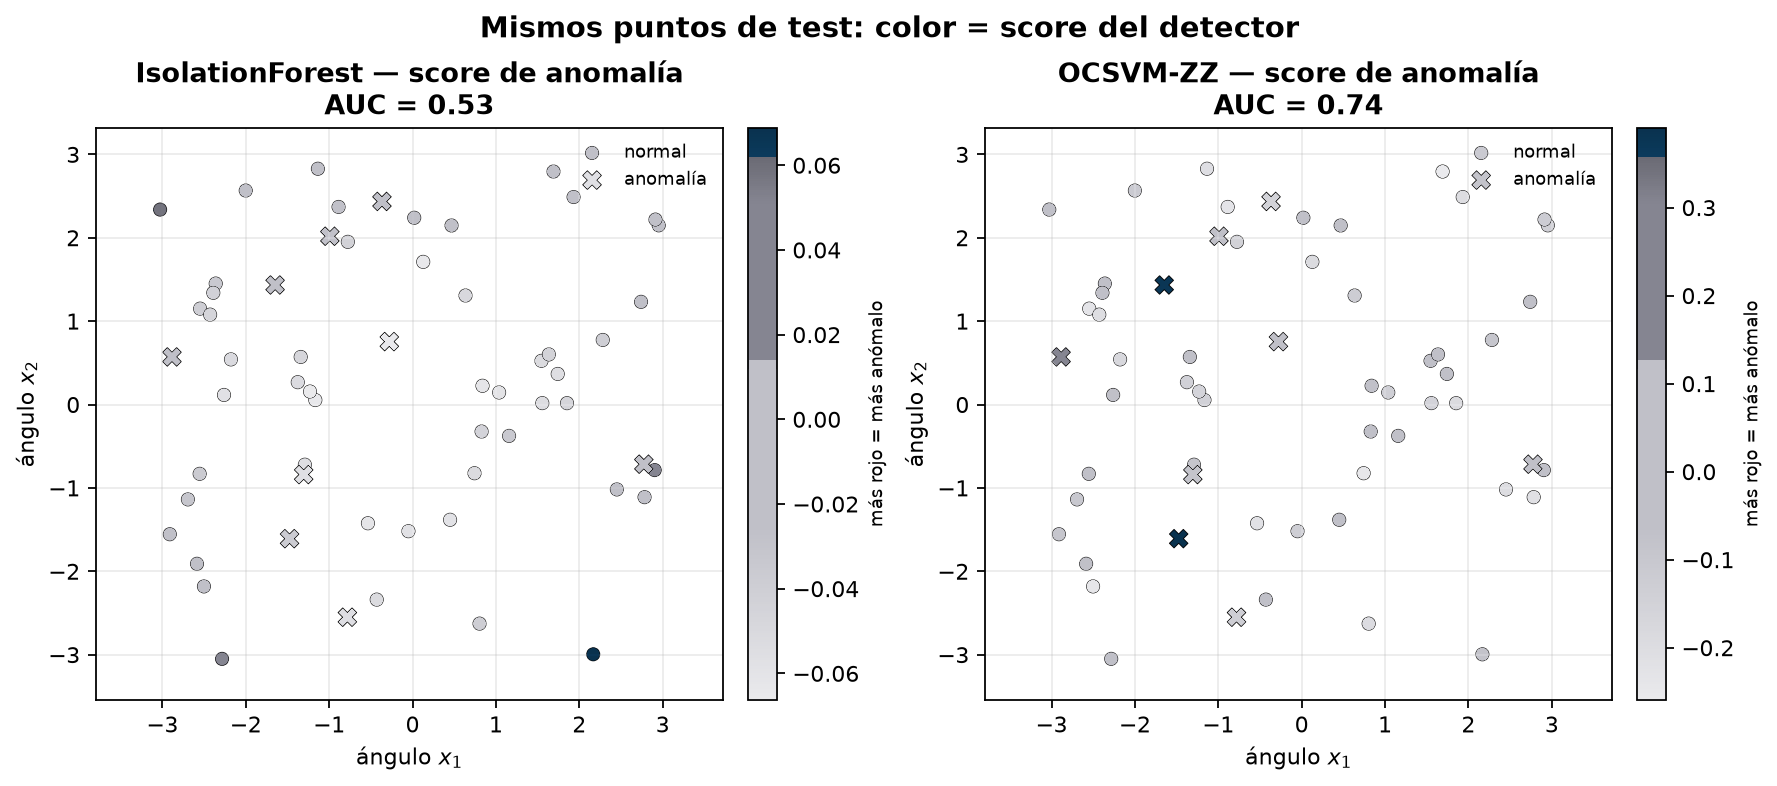
\includegraphics[width=0.98\textwidth]{Imagenes/zz_phase_scores_if_vs_zz.png}
\caption{Mismos puntos de test en \texttt{zz\_phase}: color = score de anomalía. IsolationForest obtiene AUC~$\approx 0.53$ (casi azar) y marca bordes de la nube; OCSVM-ZZ obtiene AUC~$\approx 0.74$ en este split ilustrativo (media multi-repeat $0.864$).}
\label{fig:anomaly_scores}
\end{figure}

\paragraph{Interpretación.}
La ventaja en anomalías aparece cuando lo ``raro'' \emph{no} es estar lejos, sino pertenecer a otra estructura accesible por el \textbf{feature map alineado} con el generador (aquí, fase del mapa ZZ validado empíricamente). Un mapa distinto (Pauli, IQP, \ldots) definiría otra familia de novedades beneficiadas. En tablas de práctica con spikes lejanos, IsolationForest es suficiente y más barato. El Caso~8 refuerza el mensaje transversal: el módulo cuántico es una \textbf{herramienta selectiva}, activada tras diagnóstico de alineación ($\mathcal{Q}_{\mathrm{rob}}$ / tipo de anomalía), no un sustituto por defecto de IsolationForest ni un atajo hacia ``detección de fraude cuántica''.

% =====================================================================
\section{Caso de uso 9: Forecasting one-step por lags}
\label{sec:eval_timeseries}
% =====================================================================

Los resultados de \texttt{qml\_v2.timeseries} (5 repeticiones, división temporal 70/30; Figura~\ref{fig:ts_mae}) confirman el patrón de alineación en el dominio secuencial (Tabla~\ref{tab:timeseries_dev}).

\begin{figure}[ht]
\centering
\includegraphics[width=\textwidth]{../POCs/data/output/figures/12_series_mae.png}
\caption{MAE en test (media $\pm$ desviación sobre 5 repeticiones) del Caso~9. Azul: QK-SVR-ZZ; gris oscuro: clásicos con los mismos lags (Tabla~A); gris claro: clásicos con variables adicionales (Tabla~B, marcados con *). Líneas horizontales: media del entrenamiento (discontinua) y persistencia (punteada). Fuente: \texttt{fair\_timeseries\_*.csv}, Notebook~12.}
\label{fig:ts_mae}
\end{figure}

\begin{itemize}
  \item \texttt{zz\_lag}: QK-SVR-ZZ MAE $0.056\pm0.007$ ($R^2=0.98$) frente a Ridge $0.414$, SVR-RBF $0.435$ y Gradient Boosting $0.465$; la media del entrenamiento da $0.404$, de modo que los clásicos no mejoran el predictor trivial. Ventaja por construcción: el target es $\langle ZZ\rangle$ de la ventana.
  \item \texttt{sine}: SVR-RBF $0.260$ y Ridge $0.266$ frente a QK-SVR $0.662$, que coincide con la media del entrenamiento ($0.658$). Con las variables de la Tabla~B los clásicos mejoran ligeramente ($0.244$).
  \item \texttt{skg\_speed}: Ridge $2.80\pm0.63$ frente a QK-SVR $13.59\pm5.68$ (media del entrenamiento: $13.61$). Ridge queda al nivel de la persistencia ($2.75$); con las variables de la Tabla~B el mejor clásico es Gradient Boosting ($3.24$), peor que Ridge con solo 2 lags.
\end{itemize}

\paragraph{Interpretación.}
La ventaja no es ``usar un kernel cuántico en series temporales'', sino alinear el generador del target con el feature map. Fuera del régimen nativo, el kernel ZZ con 2 qubits y $\varepsilon=0.1$ obtiene el mismo MAE que un predictor de la media del entrenamiento, es decir, no extrae señal de los lags. En la serie SKG, con solo 138 ventanas por corredor, ni siquiera los clásicos superan de forma clara a la persistencia, por lo que el valor operativo reside en el modelo lineal sobre lags y no en kernels más expresivos. ZZ es el mapa del corpus; un mapa distinto beneficiaría otra familia de series.

% =====================================================================
\section{Síntesis comparativa y discusión general}
% =====================================================================

La Tabla~\ref{tab:sintesis} sintetiza los resultados principales del estudio comparativo.

\begin{table}[ht]
\centering
\small
\setlength{\tabcolsep}{4pt}
\begin{tabular}{>{\centering\arraybackslash}p{0.7cm}>{\raggedright\arraybackslash}p{2.4cm}>{\centering\arraybackslash}p{2.5cm}>{\centering\arraybackslash}p{2.5cm}>{\centering\arraybackslash}p{2.5cm}}
\hline
\textbf{CU} & \textbf{Algoritmo cuántico} & \textbf{Cuántico-nativo} & \textbf{SKG} & \textbf{Referencia} \\
\hline
1 & QSVM & \textbf{+38.3 pp} & $-$4.5 pp & $-$3.8 pp \\
2 & QK-SVR & \textbf{$+0.965\,\Delta R^2$} & $-0.562\,\Delta R^2$ & $-0.928\,\Delta R^2$ \\
3 & QAOA ($p=1$) & \multicolumn{3}{>{\centering\arraybackslash}p{8.0cm}}{Iguala al óptimo exacto en 5/5 instancias; sin ventaja (coste idéntico)} \\
4 & VQE/QAOA & \multicolumn{3}{>{\centering\arraybackslash}p{8.0cm}}{Óptimo en 6/10 semillas (QAOA) y 3/10 (VQE) con penalización 10; Greedy y fuerza bruta, siempre ($-40$ pp)} \\
5 & QAOA TSP & \multicolumn{2}{c}{empate óptimo vs NN+2-opt ($n=4$)} & Euclidean gap~$0$ \\
6 & QSVM (umbral) & $+8.9$ pp ($n=150$, una partición) & $-4.0$ pp (clásico) & $-3.8$ pp vs GB (clásico) \\
7 & QAOA MDS ($p=3$) & \multicolumn{3}{>{\centering\arraybackslash}p{8.0cm}}{Red de 6 nodos: empate con ILP ($0$ pp); ER $n=6$--$15$: $-60$ pp de instancias con MDS óptimo (2/5 frente a 5/5)} \\
8 & OCSVM-ZZ & \textbf{+31.2 pp AUC} (\texttt{zz\_phase}) & $-29.9$ pp (inyectado) & $-29.1$ pp (moons), $-50.8$ pp (blobs) \\
9 & QK-SVR lags & \textbf{+86.6\% MAE} (\texttt{zz\_lag}) & $-385.6\%$ (\texttt{skg\_speed}) & $-154.9\%$ (\texttt{sine}) \\
\hline
\end{tabular}
\caption{Síntesis cuántico vs clásico, generada por \texttt{scripts/sintesis\_resultados.py} a partir de las salidas ejecutadas. Positivo = favorece al método cuántico; unidades: pp de exactitud (CU1, CU6), $\Delta R^2$ (CU2), pp de AUC (CU8) y mejora relativa del MAE (CU9). Negrita = ventaja sobre el mejor clásico. En kernels, la ventaja aparece \textbf{solo} en el régimen cuántico-nativo (datos generados por el propio mapa); en SKG y Telco gana GB/RF (Telco $-3.8$~pp frente a Gradient Boosting). Los Casos~1, 2 y~6 usan una sola partición con 45--60 puntos de test (granularidad de $\pm2.2$~pp).}
\label{tab:sintesis}
\end{table}

\begin{figure}[!htbp]
\centering
\begin{tikzpicture}[font=\small, thick,
    bg/.style={rectangle, rounded corners=3pt, minimum width=1.3cm, minimum height=0.7cm, align=center},
    verde/.style={bg, fill=green!22, draw=green!55!black},
    amarillo/.style={bg, fill=yellow!30, draw=yellow!65!black},
    rojo/.style={bg, fill=red!18, draw=red!50!black},
    header/.style={font=\bfseries\footnotesize, align=center}]

  % Columnas: x = 0(CU), 2.2(Algoritmo), 5.5(Resultado), 8.2(Escala NISQ), 10.9(Valor SKG)
  \node[header] at (0,    0) {CU};
  \node[header] at (2.4,  0) {Algoritmo cuántico};
  \node[header] at (5.6,  0) {Resultado\\ Q vs C};
  \node[header] at (8.3,  0) {Escalabilidad\\ NISQ};
  \node[header] at (11.0, 0) {Valor\\ para SKG};

  \draw[gray!40, thick] (-0.5, -0.42) -- (12.3, -0.42);

  % Fila 1 – CU1
  \node[font=\footnotesize] at (0,    -1.0) {1};
  \node[font=\footnotesize, align=left] at (2.4, -1.0) {QSVM};
  \node[verde]    at (5.6,  -1.0) {\scriptsize Ventaja};
  \node[amarillo] at (8.3,  -1.0) {\scriptsize Moderada};
  \node[amarillo] at (11.0, -1.0) {\scriptsize Moderado};

  % Fila 2 – CU2
  \node[font=\footnotesize] at (0,    -1.9) {2};
  \node[font=\footnotesize, align=left] at (2.4, -1.9) {QK-SVR};
  \node[rojo]     at (5.6,  -1.9) {\scriptsize Desventaja};
  \node[amarillo] at (8.3,  -1.9) {\scriptsize Moderada};
  \node[rojo]     at (11.0, -1.9) {\scriptsize Bajo};

  % Fila 3 – CU3
  \node[font=\footnotesize] at (0,    -2.8) {3};
  \node[font=\footnotesize, align=left] at (2.4, -2.8) {QAOA ($p{=}1$)};
  \node[amarillo] at (5.6,  -2.8) {\scriptsize Empate};
  \node[amarillo] at (8.3,  -2.8) {\scriptsize Moderada};
  \node[amarillo] at (11.0, -2.8) {\scriptsize Moderado};

  % Fila 4 – CU4
  \node[font=\footnotesize] at (0,    -3.7) {4};
  \node[font=\footnotesize, align=left] at (2.4, -3.7) {VQE / QAOA};
  \node[rojo]     at (5.6,  -3.7) {\scriptsize Desventaja};
  \node[amarillo] at (8.3,  -3.7) {\scriptsize Moderada};
  \node[amarillo] at (11.0, -3.7) {\scriptsize Moderado};

  % Fila 5 – CU5
  \node[font=\footnotesize] at (0,    -4.6) {5};
  \node[font=\footnotesize, align=left] at (2.4, -4.6) {QAOA TSP};
  \node[amarillo] at (5.6,  -4.6) {\scriptsize Empate ópt.};
  \node[rojo]     at (8.3,  -4.6) {\scriptsize Limitada};
  \node[amarillo] at (11.0, -4.6) {\scriptsize Selectivo};

  % Fila 6 – CU6
  \node[font=\footnotesize] at (0,    -5.5) {6};
  \node[font=\footnotesize, align=left] at (2.4, -5.5) {QSVM (umbral)};
  \node[amarillo] at (5.6,  -5.5) {\scriptsize Condicional};
  \node[amarillo] at (8.3,  -5.5) {\scriptsize Moderada};
  \node[amarillo] at (11.0, -5.5) {\scriptsize Moderado};

  % Fila 7 – CU7
  \node[font=\footnotesize] at (0,    -6.4) {7};
  \node[font=\footnotesize, align=left] at (2.4, -6.4) {QAOA MDS};
  \node[rojo]     at (5.6,  -6.4) {\scriptsize Desventaja};
  \node[amarillo] at (8.3,  -6.4) {\scriptsize Moderada};
  \node[amarillo] at (11.0, -6.4) {\scriptsize Moderado};

  % Fila 8 – CU8
  \node[font=\footnotesize] at (0,    -7.3) {8};
  \node[font=\footnotesize, align=left] at (2.4, -7.3) {OCSVM-ZZ};
  \node[amarillo] at (5.6,  -7.3) {\scriptsize Condicional};
  \node[amarillo] at (8.3,  -7.3) {\scriptsize Moderada};
  \node[amarillo] at (11.0, -7.3) {\scriptsize Selectivo};

  % Fila 9 – CU9
  \node[font=\footnotesize] at (0,    -8.2) {9};
  \node[font=\footnotesize, align=left] at (2.4, -8.2) {QK-SVR lags};
  \node[amarillo] at (5.6,  -8.2) {\scriptsize Condicional};
  \node[amarillo] at (8.3,  -8.2) {\scriptsize Moderada};
  \node[amarillo] at (11.0, -8.2) {\scriptsize Selectivo};

  % Leyenda
  \node[verde,    minimum width=0.9cm] (lg) at (2.0, -9.3) {};
  \node[right=4pt, font=\scriptsize] at (lg.east) {Favorable / Ventaja cuántica};
  \node[amarillo, minimum width=0.9cm] (ly) at (6.5, -9.3) {};
  \node[right=4pt, font=\scriptsize] at (ly.east) {Moderado / Empate};
  \node[rojo,     minimum width=0.9cm] (lr) at (10.2, -9.3) {};
  \node[right=4pt, font=\scriptsize] at (lr.east) {Desfavorable};

\end{tikzpicture}
\caption{Semáforo de resultados por caso de uso. Azul = favorable; gris claro = moderado, empate o condicional; gris = desfavorable. La columna ``Resultado'' se deriva de la Tabla~\ref{tab:sintesis}; ``Escalabilidad NISQ'' y ``Valor para SKG'' son valoraciones cualitativas del autor, no mediciones. Los Casos~8 y~9 son condicionales: hay ventaja cuando novedad o target están alineados con el feature map (aquí ZZ). Caso~7: empate en la red de 6 nodos y $-60$~pp de instancias con MDS óptimo en los grafos ER.}
\label{fig:semaforo_resultados}
\end{figure}

\clearpage
\begin{figure}[!htbp]
\centering
\includegraphics[width=0.97\textwidth]{../POCs/data/output/figures/07_dashboard_ventaja_cuantica.png}
\caption{Dashboard de los nueve casos de uso, generado a partir de \texttt{07\_sintesis\_resultados.csv}. Cada panel usa la unidad de su caso (pp de exactitud, $\Delta R^2\times100$, \% de coste, pp de AUC, \% de MAE o pp de instancias con MDS óptimo); positivo favorece al método cuántico. Azul = ventaja cuántica; gris = clásico superior; gris claro = empate. Coherente con la Tabla~\ref{tab:sintesis}.}
\label{fig:dashboard_sintesis}
\end{figure}

\begin{figure}[!htbp]
\centering
\includegraphics[width=0.90\textwidth]{../POCs/data/output/figures/07_heatmap_ventaja_por_dominio.png}
\caption{Mapa de calor de la ventaja cuántica sobre el mejor clásico por caso de uso y tipo de dataset, con la unidad indicada en cada fila; el color se satura en $\pm80$ y la anotación conserva el valor real. Las celdas azules aparecen solo con alineación feature map--generador (Casos~1, 2, 6, 8 y~9 en datos nativos). Las celdas grises reflejan dominio clásico. Los Casos~3, 4 y~5 no distinguen tipo de dataset y se sitúan en la columna de referencia; el Caso~7 se mide en pp de instancias con MDS óptimo frente a ILP/Greedy y se sitúa en la columna de referencia.}
\label{fig:heatmap_ventaja_body}
\end{figure}

\begin{figure}[!htbp]
\centering
\includegraphics[width=0.95\textwidth]{../POCs/data/output/figures/07_grover_benchmark.png}
\caption{Conteo teórico de operaciones del algoritmo de Grover ($\lfloor\pi\sqrt{N}/4\rfloor$ iteraciones) frente a la búsqueda clásica no estructurada ($N$ comparaciones) en función del tamaño del espacio de búsqueda $N$. Es una ilustración analítica: no se ejecutó Grover ni se midió tiempo, y no incluye el coste del oráculo. La aceleración cuadrática se hace evidente a partir de $N \approx 10^3$, ilustrando el tipo de ventaja estructural que la computación cuántica puede aportar a problemas de búsqueda y optimización.}
\label{fig:grover_benchmark}
\end{figure}

\begin{figure}[!htbp]
\centering
\includegraphics[width=0.95\textwidth]{../POCs/data/output/figures/07_paralelismo_cuantico.png}
\caption{Superposición de $n$ qubits tras aplicar Hadamard a $|0\rangle^{\otimes n}$: el vector de estado tiene $2^n$ amplitudes iguales ($1/2^n$ de probabilidad cada una). Que el espacio de Hilbert crezca exponencialmente no implica que el computador cuántico evalúe $2^n$ casos a la vez: una medición devuelve un único resultado, y la ventaja de algoritmos como Grover o Shor proviene de la interferencia, no del mero paralelismo.}
\label{fig:paralelismo_cuantico}
\end{figure}

\subsection{Patrones transversales}

Los resultados evidencian tres patrones transversales que son coherentes con el estado actual de la teoría y la tecnología cuántica:

\begin{enumerate}
  \item \textbf{La ventaja cuántica requiere alineación dato--feature map}: La ventaja observada en datos nativos es coherente con \cite{huang2021}: el feature map (ZZ u otro) debe estar alineado con el generador; ZZ es el mapa validado empíricamente en este TFM, no un monopolio. En datos reales sin esa alineación, Gradient Boosting y Random Forest mantienen su superioridad.

  \item \textbf{El cuello de botella es la escala}: En todos los casos, la principal limitación práctica del enfoque cuántico no es la calidad del algoritmo sino el coste cuadrático del kernel ($O(n^2)$) y el número de qubits disponibles \citep{haug2023, cerezo2021}. Esta limitación es una función del hardware actual, no del algoritmo en sí.

  \item \textbf{Los resultados negativos son informativos}: Los casos donde el QSVM o el QK-SVR son inferiores a los clásicos en datos reales no son fracasos experimentales, sino resultados metodológicamente valiosos que delimitan el dominio de aplicabilidad. El Caso~8 añade el mismo matiz en one-class: OCSVM-ZZ no sustituye IsolationForest salvo cuando la novedad está alineada con el mapa (aquí \texttt{zz\_phase}), no cuando es geométrica clásica.
\end{enumerate}

\subsection{Implicaciones para la adopción empresarial}

Desde la perspectiva de SKG Tecnología, los resultados sugieren que la integración de algoritmos cuánticos en los sistemas de gestión de movilidad urbana requiere dos condiciones previas: (i) hardware cuántico con mayor número de qubits lógicos y menor tasa de error \citep{preskill2018, cerezo2023}, para operar sobre más features sin reducción dimensional, y (ii) ingeniería de features específica que alinee la representación de los datos con las estructuras geométricas accesibles por los kernels cuánticos \citep{huang2021}. En el corto plazo (horizonte 2--5 años), el valor más realista de la computación cuántica para SKG reside en los algoritmos de optimización combinatoria (QAOA, VQE) para problemas de asignación de recursos, aunque en los casos medidos aquí (3, 4, 5 y 7) ningún solver cuántico ha superado a los exactos \citep{farhi2014}.

El hilo conductor de los nueve casos de uso es precisamente la demostración de que los algoritmos cuánticos no necesitan reemplazar a los clásicos para ser útiles: basta con que resuelvan de forma más eficaz la parte del problema que es intratable para la computación clásica \citep{biamonte2017}. El Caso~7 lo ilustra de forma paradigmática: aplicar QAOA al conjunto dominante mínimo ---un problema NP-difícil--- y conectarlo con un optimizador clásico COBYLA a través de una interfaz mínima es exactamente el patrón con el que la computación cuántica puede integrarse en entornos productivos reales \citep{farhi2014}. El prototipo de arquitectura híbrida desarrollado en la Sección~\ref{sec:prototipo_hibrido} del Capítulo~\ref{cap:metodologia} formaliza este patrón y define los criterios de activación del módulo cuántico según el tipo de problema.

\subsection{Resultados adicionales y visualización}

El análisis de escalabilidad del caso~1 se sintetiza en la Figura~\ref{fig:escala_clasificacion}: ventaja positiva en $n \in [30, 180]$ (10 repeticiones por tamaño) \textbf{solo} en el régimen cuántico-nativo. La geometría de kernel se reporta vía los indicadores tabulares del Capítulo~\ref{cap:investigacion_original} ($\Delta A$, $d_F$, $\Delta H$); no se usan heatmaps regenerados a posteriori (las matrices $K$ no se exportaron a artefactos). $\mathcal{Q}>0$ vs.\ un baseline débil no basta como veredicto operativo.


% !TEX root = ../main.tex
\chapter{Tests de Cuanticidad y Mapeos Cuántico-Compatibles}
\label{cap:investigacion_original}

Los capítulos anteriores han mostrado un patrón consistente: la ventaja cuántica en kernels aparece con robustez cuando el \textbf{generador del dato está alineado con el feature map} del kernel ---en los experimentos de este TFM, datos sintéticos generados con el \texttt{ZZFeatureMap} de modo que ese kernel es óptimo por construcción---, y desaparece en datos reales de movilidad y telecomunicaciones sin esa alineación. ZZ no es el único mapa posible (Pauli, IQP, re-uploading, etc.); es el que se validó empíricamente aquí. Este resultado plantea dos preguntas que este capítulo aborda como contribución original del TFM:

\begin{enumerate}
    \item \textbf{Tests de cuanticidad}: \textquestiondown{}Existe algún indicador calculable a priori sobre un dataset que permita predecir si un algoritmo cuántico mostrará ventaja sobre los clásicos?
    \item \textbf{Mapeos cuántico-compatibles}: Si un dataset no tiene estructura cuántica nativa, \textquestiondown{}puede transformarse a un espacio de representación donde la tenga, sin alterar la información discriminativa?
\end{enumerate}

Ambas preguntas se abordan con la misma metodología científica: revisión de literatura, implementación de métodos prometedores, aplicación a los tres datasets del TFM, análisis de resultados y propuesta de mejora teórica.

% =====================================================================
\section{Tests de cuanticidad: revisión de la literatura}
\label{sec:lit_cuanticidad}
% =====================================================================

\subsection{El problema de la selección de algoritmo a priori}

El problema de seleccionar el algoritmo más adecuado antes del entrenamiento es un problema clásico en aprendizaje automático, tratado bajo el marco del \textit{No Free Lunch Theorem} \citep{wolpert1997}. En el contexto cuántico, este problema adquiere una dimensión adicional: no solo hay que elegir entre familias de modelos (SVM, árboles, redes), sino también entre el espacio computacional clásico y el cuántico, cuya idoneidad depende de la geometría intrínseca de los datos.

\subsection{Kernel alignment como indicador de alineación estructural}

El \textit{kernel alignment} \citep{cortes2012} es una medida de la correspondencia entre la geometría inducida por un kernel y la estructura de clases de un dataset. Formalmente, dado un kernel $K$ y la matriz de etiquetas $K_y = yy^T$, se define:

\begin{equation}
    A(K, K_y) = \frac{\langle K, K_y \rangle_F}{\|K\|_F \cdot \|K_y\|_F}
    \label{eq:kernel_alignment}
\end{equation}

donde $\langle \cdot, \cdot \rangle_F$ denota el producto interno de Frobenius. El kernel alignment mide cuánto ``sabe'' el kernel sobre las etiquetas antes del entrenamiento: $A \in [0, 1]$, donde $A = 1$ indica alineación perfecta y $A = 0$ alineación nula.

\citet{huang2021} adaptaron este concepto al contexto cuántico, proponiendo el \textit{geometric difference} $g(K_Q, K_{cl})$ como medida de la separación entre los espacios de características cuántico y clásico. Su resultado teórico central acota el error de predicción de un modelo de kernel mediante su complejidad $s_K(N)$ y establece que, si $g$ es pequeña, un modelo clásico tiene una complejidad, y por tanto un error de predicción, similar o mejor que el cuántico, con independencia de las etiquetas. Una $g$ grande es solo una condición necesaria: garantiza que existe un conjunto de etiquetas con ventaja cuántica, no que el dataset real la tenga.

\begin{figure}[ht]
\centering
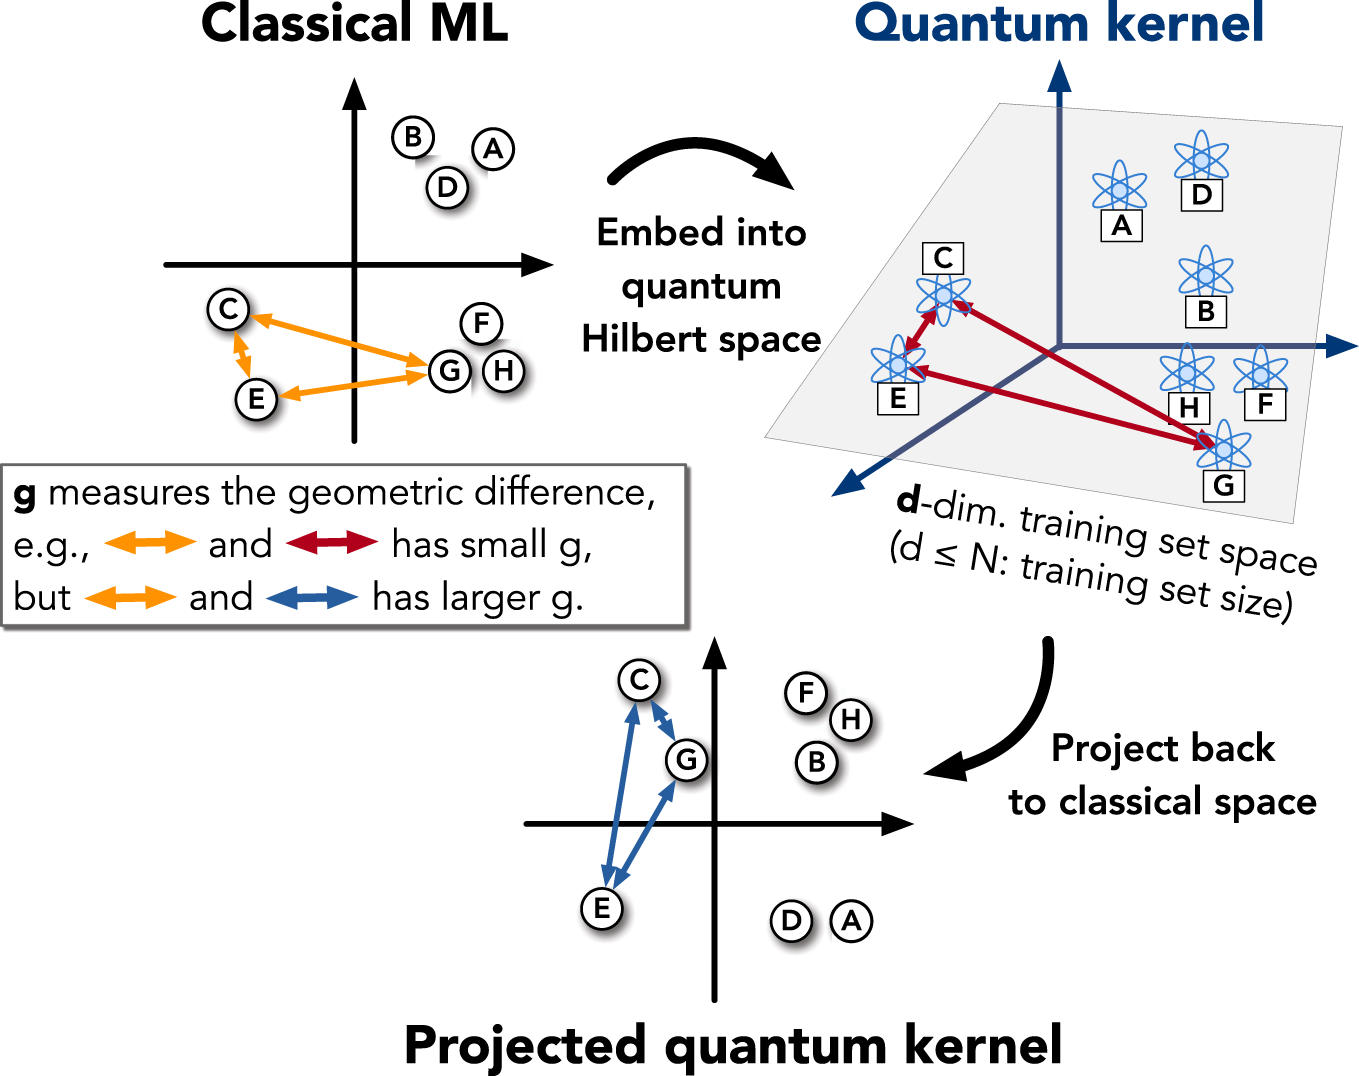
\includegraphics[width=0.62\textwidth]{Imagenes/huang2021_fig2_geometria_kernel.png}
\caption{Geometría del kernel clásico y cuántico. Las letras A, B, \dots{} son puntos de datos $\{x_i\}$ en espacios distintos; las flechas representan la similitud (función kernel) entre datos. La diferencia geométrica $g$ compara las similitudes entre modelos (flechas naranja/roja: $g$ pequeño; naranja/azul: $g$ mayor) y $d$ es una dimensión efectiva del conjunto de datos en el espacio de Hilbert cuántico. Reproducida de \citet{huang2021}, Fig.~2, bajo licencia CC~BY~4.0.}
\label{fig:huang_geometria}
\end{figure}

\subsection{Concentración exponencial y entropía espectral}

\citet{thanasilp2022} identificaron que los kernels cuánticos exhiben \textit{concentración exponencial} bajo cuatro condiciones: alta expresividad del mapa de datos, mediciones globales, entrelazamiento excesivo y ruido. La concentración implica que todos los valores del kernel convergen a una constante, lo que destruye la información discriminativa.

Un indicador directo de concentración es la \textbf{entropía espectral} de la matriz de Gram $K_Q$. Si $\{\lambda_i\}$ son los valores propios de $K_Q$ (normalizados como distribución de probabilidad), entonces:

\begin{equation}
    H(K_Q) = -\sum_{i} \hat{\lambda}_i \log \hat{\lambda}_i, \quad \hat{\lambda}_i = \frac{\lambda_i}{\sum_j \lambda_j}
    \label{eq:spectral_entropy}
\end{equation}

Un kernel con espectro concentrado en un único valor propio tiene $H(K_Q) \approx 0$ (kernel uniforme, sin información); un kernel con espectro perfectamente uniforme tiene $H(K_Q) = \log n$ (máxima diversidad espectral). La hipótesis es que datasets con ventaja cuántica exhiben $H(K_Q) \gg H(K_{RBF})$.

\subsection{Divergencia cuántica-clásica en el espacio de kernels}

\citet{liu2021} demostraron, bajo la conjetura de dificultad del logaritmo discreto, que existe un problema de clasificación que un kernel cuántico aprende de forma eficiente y que ningún algoritmo clásico eficiente puede aprender. De ahí se desprende que una ventaja de este tipo exige un kernel difícil de aproximar clásicamente. Un proxy operativo, definido en este trabajo y no propuesto por esos autores, es la \textbf{distancia de Frobenius normalizada}:

\begin{equation}
    d_F(K_Q, K_{cl}) = \frac{\|K_Q - K_{cl}^*\|_F}{n}
    \label{eq:frobenius_dist}
\end{equation}

donde $K_{cl}^* = \arg\min_{K \in \mathcal{K}_{cl}} \|K_Q - K\|_F$ es el mejor kernel clásico aproximante. En la práctica, $K_{cl}^*$ se aproxima buscando el mejor $\sigma$ del kernel RBF. Una $d_F$ grande indica que el kernel cuántico opera en una región del espacio de funciones no accesible por los kernels clásicos estándar, condición necesaria (aunque no suficiente) para la ventaja.

\subsection{Métricas de expresividad del circuito}

\citet{sim2019} definieron la \textit{expressibility} de un ansatz cuántico como la capacidad de sus estados para explorar el espacio de Hilbert. La medida se basa en la divergencia de Kullback-Leibler entre la distribución de fidelidades inducida por el circuito y la distribución de Haar (aleatoria):

\begin{equation}
    \text{Expr} = D_{KL}(\hat{P}_{PQC}(F; \theta) \,\|\, P_{Haar}(F))
    \label{eq:expressibility}
\end{equation}

Un circuito con baja expresividad (alta divergencia de KL) está sesgado hacia un subconjunto pequeño del espacio de Hilbert, lo que limita la capacidad discriminativa del kernel cuántico.

\subsection{Cota de ventaja basada en datos (Huang et al., 2021)}

\citet{huang2021} propusieron un diagrama de decisión para evaluar la ventaja potencial de un modelo cuántico con un número fijo de datos de entrenamiento. Dado un kernel $K$ y $N$ datos, el error de predicción está acotado por $c\sqrt{s_K(N)/N}$, donde $s_K(N)=\lVert w\rVert^2$ es la complejidad del modelo entrenado. Para dos kernels $K_1$ y $K_2$ con $\mathrm{Tr}\,K_1=\mathrm{Tr}\,K_2=N$ se cumple

\begin{equation}
    s_{K_1}(N) \leq g(K_1\Vert K_2)^2\, s_{K_2}(N),
    \qquad
    g(K_1\Vert K_2)=\sqrt{\bigl\lVert \sqrt{K_2}\,K_1^{-1}\sqrt{K_2}\bigr\rVert_\infty},
    \label{eq:huang_bound}
\end{equation}

de modo que, si $g(K_C\Vert K_Q)$ es pequeña, el modelo clásico es competitivo o mejor que el cuántico. Si es grande, existe un conjunto de etiquetas para el que el modelo cuántico predice mejor, pero eso no implica que ocurra en un dataset concreto. Este resultado liga los indicadores de geometría de kernels con cotas de error de predicción, y es la base teórica de la diferencia geométrica $g$ usada en este trabajo; no es un test estadístico de significación.

% =====================================================================
\section{Resultados prometedores de la literatura}
\label{sec:lit_resultados}
% =====================================================================

La Tabla~\ref{tab:lit_indicadores} resume los indicadores propuestos en la literatura, su fundamento teórico, su complejidad computacional y su conexión con la ventaja cuántica demostrada.

\begin{table}[ht]
\centering
\small
\begin{tabular}{>{\raggedright\arraybackslash}p{3.1cm}>{\raggedright\arraybackslash}p{2.7cm}>{\raggedright\arraybackslash}p{2.5cm}>{\raggedright\arraybackslash}p{4.0cm}}
\hline
\textbf{Indicador} & \textbf{Base conceptual} & \textbf{Complejidad} & \textbf{Relación con la literatura} \\
\hline
Kernel alignment $A(K_Q, K_y)$ & \citet{cortes2012, huang2021} & $O(n^2)$ & Mide el ajuste kernel--etiquetas; no es por sí sola condición de ventaja \\
Entropía espectral $H(K_Q)$ & \citet{thanasilp2022} & $O(n^3)$ & Proxy propio de la concentración del kernel descrita por esos autores \\
Distancia Frobenius $d_F$ & \citet{liu2021} & $O(n^2)$ & Proxy propio de la dificultad de aproximación clásica \\
Diferencia geométrica $g$ & \citet{huang2021} & $O(n^2)$ & Aparece en la cota $s_{K_1}\leq g^2 s_{K_2}$ de la Ec.~\ref{eq:huang_bound} \\
Expressibility & \citet{sim2019} & $O(2^n)$ & Capacidad de exploración del espacio de Hilbert \\
\hline
\end{tabular}
\caption{Indicadores de cuanticidad propuestos en la literatura, con su referencia original, complejidad y base teórica.}
\label{tab:lit_indicadores}
\end{table}

La literatura \citep{huang2021, thanasilp2022, schuld2021kernels} indica que ningún indicador individual es condición suficiente para la ventaja; la combinación de $A(K_Q, K_y) > A(K_{cl}, K_y)$ (el kernel cuántico está más alineado con las etiquetas) y $d_F > \epsilon$ (el kernel cuántico es genuinamente diferente del clásico) es la combinación que se adopta como criterio operativo en este trabajo.

% =====================================================================
\section{Aplicación a los datasets del TFM}
\label{sec:aplicacion_cuanticidad}
% =====================================================================

Se implementaron los cinco indicadores anteriores sobre los tres datasets del TFM utilizando el Notebook~08 (\texttt{08\_test\_cuanticidad\_datasets.ipynb}). Para cada dataset se calculó la matriz de kernel cuántico $K_Q$ (ZZFeatureMap, 2 qubits, tras reducción PCA a 2 dimensiones) y la mejor matriz de kernel clásico $K_{RBF}^*$ (búsqueda de $\sigma$ óptimo por validación cruzada).

\subsection{Resultados cuantitativos}

\begin{table}[ht]
\centering
\small
\begin{tabular}{lccccccc}
\hline
\textbf{Dataset} & $A(K_Q,K_y)$ & $A(K_{cl},K_y)$ & $H(K_Q)$ & $H(K_{cl})$ & $d_F$ & $\Delta_{\mathrm{RBF}}$ & \textbf{$\Delta_{\mathrm{op}}$} \\
\hline
Cuántico-nativo  & 0.027 & 0.056 & 2.307 & 3.427 & 0.358 & $+4.2$ & $\mathbf{+8.9}$ \\
SKG Incidentes   & 0.040 & 0.050 & 2.155 & 1.967 & 0.369 & $+8.3^\dagger$ & $\mathbf{-4.0}$ \\
Telco Churn      & 0.190 & 0.170 & 2.333 & 3.465 & 0.346 & $+$0.0 & $\mathbf{-3.8}$ \\
\hline
\end{tabular}
\caption{Indicadores de cuanticidad (Notebook~08, ZZFeatureMap 2~qubits, PCA~2D, $n=80$). Geometría vs.\ kernel clásico de referencia; $\Delta_{\mathrm{RBF}}$ = QSVM$-$SVM-RBF en el split NB08 (baseline débil). Columna $\Delta_{\mathrm{op}}$ = accuracy(QSVM)$-$accuracy(\textbf{mejor clásico}) en \textbf{clasificación} (Notebook~06): nativo $+8.9$~pp, SKG $-4.0$~pp, Telco $-3.8$~pp vs Gradient Boosting --- no es una métrica geométrica. Los indicadores del dataset nativo dependen del etiquetado por autovector del kernel, que es sensible al \emph{backend} numérico (véase la nota siguiente). $^\dagger$SKG $+8.3$~pp vs RBF es artefacto ---bajo $\mathcal{Q}_{\mathrm{rob}}$ y frente al stack clásico SKG es \texttt{classical}.}
\label{tab:indicadores_resultados}
\end{table}

\paragraph{Sensibilidad numérica del dataset nativo.}
En el Notebook~08 las etiquetas del dataset nativo se definen por el signo de un autovector de $K_Q$, elección que es inestable cuando hay autovalores casi degenerados. Al reejecutar el cuaderno de principio a fin (Qiskit~2.6.1, NumPy~2.5) los indicadores de ese dataset cambiaron respecto a la ejecución original ($\Delta H$ de $+0.034$ a $-1.120$, $\mathcal{Q}$ de $+0.286$ a $-0.056$, $\Delta_{\mathrm{RBF}}$ de $0.0$ a $+4.2$~pp), mientras que SKG, Telco y el barrido $\alpha$ se reprodujeron exactamente. La tabla recoge las cifras reejecutadas; la conclusión es que $\Delta H$ y $\mathcal{Q}$ del dataset nativo \textbf{no} son estables frente al entorno numérico y no deben leerse como una propiedad del dataset.

\subsection{Figuras de resultados}

\begin{figure}[ht]
\centering
\includegraphics[width=0.95\textwidth]{../POCs/data/output/figures/08_test_cuanticidad_datasets.png}
\caption{Perfil vectorial $\mathcal{Q}(\mathcal{D})=(\Delta A,d_F,\Delta H)$ sobre los tres datasets (Notebook~08). Fila superior: componentes del vector. Fila inferior: alineaciones, entropías de apoyo y el escalar ponderado $w^\top\mathcal{Q}$ (experimento; \textbf{no} regla de adopción). Telco y nativo dominados por $\Delta H$ ($-1.131$ y $-1.120$). La decisión operativa usa $\Delta_{\mathrm{op}}$ (Tabla~\ref{tab:indicadores_resultados}), no el escalar.}
\label{fig:indicadores_cuanticidad}
\end{figure}

\paragraph{Nota sobre visuales de matrices de kernel.}
Las matrices $K_Q$/$K_{cl}$ viven en memoria durante la ejecución del Notebook~08 y \textbf{no se serializaron} como artefactos. Un heatmap o ``contraste de bloques'' regenerado a posteriori (sin re-ejecutar el notebook) sería construcción ilustrativa, no medición. Por criterio de este TFM (\emph{nada forzado ni construido a mano}) esa figura se \textbf{retira} del cuerpo; la geometría se reporta solo vía los indicadores tabulares ($d_F$, $g$, $\Delta A$, $\Delta H$).

\subsection{Análisis: \textquestiondown{}Predicen los indicadores la ventaja QSVM?}

La Tabla~\ref{tab:indicadores_resultados} distingue dos rankings. Bajo el protocolo NB08 vs.\ un baseline RBF débil: SKG ($+8.3$~pp) $>$ nativo ($+4.2$~pp) $>$ Telco ($0.0$~pp) ---ranking \textbf{engañoso}. El ranking operativo vs.\ mejor clásico es: \textbf{nativo ($+8.9$~pp)} $>$ Telco ($-3.8$~pp) $>$ SKG ($-4.0$~pp). Solo el régimen cuántico-nativo muestra ventaja; SKG/Telco son clásicos (Sección~\ref{sec:qml_v2_revision}).

El score $\mathcal{Q}(\mathcal{D})$ (calculado vs.\ kernel clásico de referencia) ordena SKG ($+0.352$) $>$ Telco ($-0.050$) $>$ nativo ($-0.056$): el único dataset con ventaja operativa queda el último. Frente al ranking vs.\ RBF la relación es débil ($\rho_S=+0.5$, $n=3$) y frente al ranking operativo es inversa ($\rho_S=-1.0$ entre $\mathcal{Q}$ y $\Delta_{\mathrm{op}}$, $n=3$): en esta implementación, con 2 qubits y PCA a 2 dimensiones, $\mathcal{Q}$ \textbf{no} identifica el régimen nativo. El barrido sintético NB08 ($n=9$, $X$ fijo + mezcla de etiquetas) muestra $\rho_S(\alpha,\Delta A)=+0.833$ ($p=0.005$): resultado esperable por construcción, ya que mezclar etiquetas cuánticas aumenta la alineación con el kernel. Bajo ese protocolo $d_F$ y $H$ son constantes, y $\rho_S(\alpha,\mathrm{ventaja})\approx 0.34$ (n.s.) ---\textbf{no} se afirma que $\mathcal{Q}$ prediga ventaja con $\rho=0.833$. Lectura: $\mathcal{Q}>0$ vs.\ un baseline débil \textbf{no} autoriza desplegar el módulo cuántico.

El análisis individual de los componentes revela matices importantes:
\begin{itemize}
    \item $\Delta A$ es negativa en dos de los tres datasets en el régimen 2~qubits + PCA. Frente a $\Delta_{\mathrm{op}}$, $\rho_S(\Delta A,\Delta_{\mathrm{op}})=-0.500$ ($n=3$); en el barrido NB08 $\rho_S(\alpha,\Delta A)=+0.833$: el PCA agresivo suprime la señal de $\Delta A$ en datos reales.
    \item $d_F$ y $g$ frente a $\Delta_{\mathrm{op}}$ dan $\rho_S=-0.5$ y $-1.0$ ($n=3$): no sustituyen la comparación contra el mejor clásico ni el veredicto $\mathcal{Q}_{\mathrm{rob}}$.
    \item $\Delta H$ es el indicador más volátil: $\mathcal{Q}$ de Telco y del nativo están dominados por $\Delta H=-1.131$ y $-1.120$ (concentración espectral).
\end{itemize}

\paragraph{Caveat estadístico.}
Con $n=3$ datasets, cualquier $\rho_S$ es de potencia baja (máximo $\pm 1$ o $\pm 0.5$ con empates). El $\rho_S=+0.833$ del barrido es $\rho(\alpha,\Delta A)$, no $\rho(\mathcal{Q},\mathrm{ventaja})$. La validación sobre más datasets y un barrido structure-aware (donde $d_F$/$H$ también varíen) es trabajo futuro explícito (Capítulo~\ref{cap:futuro}).

\paragraph{Debilidades metodológicas expuestas (integridad de resultados).}
Un buen TFM se discute desde lo medido, no desde lo deseable. Aquí se exponen límites \textbf{sin alterar cifras}:
\begin{itemize}
    \item Barrido $\alpha$ con $X$ fijo: $d_F$, $H$ y $g$ constantes ---no valida monotonía de todos los factores de $\mathcal{Q}$.
    \item Ventaja NB08 vs.\ RBF en SKG ($+8.3$~pp) es artefacto de baseline débil; el $\Delta_{\mathrm{op}}$ viene de otro protocolo (Caso~1 / NB06) y \textbf{no} se mezcla en la misma $\rho$.
    \item $n=3$ no sostiene correlaciones fuertes entre $\mathcal{Q}$ y ventaja operativa.
    \item No hay dumps de $K$ en artefactos: no se inventan heatmaps.
    \item Series de rotación NB09: PNG del notebook; no regenerar con curvas proxy.
    \item Componentes $\Delta A$/$d_F$/$\Delta H$ \emph{post} re-uploading no están en el log NB09: no se inventan (solo $Q$ y Adv post están verificados).
\end{itemize}

\begin{figure}[ht]
\centering
\includegraphics[width=0.92\textwidth]{../POCs/data/output/figures/08_barrido_sintetico_alpha.png}
\caption{Barrido sintético NB08 (datos reales): $\alpha$ = fracción de etiquetas cuánticas con $X$ fijo. $\Delta A$ crece con $\alpha$ ($\rho_S=+0.833$, $p=0.005$). $d_F$ y $H(K_Q)$ son constantes por diseño (los kernels no dependen de las etiquetas). La ventaja supervisada es ruidosa ($\rho_S(\alpha,\mathrm{ventaja})\approx 0.34$). El número $0.833$ es $\rho(\alpha,\Delta A)$, \textbf{no} $\rho(\mathcal{Q},\mathrm{ventaja})$.}
\label{fig:barrido_sintetico_alpha}
\end{figure}

\begin{figure}[!htbp]
\centering
\includegraphics[width=0.88\textwidth]{../POCs/data/output/figures/08_correlacion_indicadores_ventaja.png}
\caption{Indicadores NB08 vs.\ ventaja NB08 (QSVM$-$SVM-RBF, puntos rellenos). Marcadores huecos: $\Delta_{\mathrm{op}}$ de Caso~1/NB06 (referencia; \textbf{no} entran en $\rho$). Línea gris: barrido $\alpha$ solo en el panel $\Delta A$ (único factor que varía con $X$ fijo). $n=3$: potencia baja; no se reclama $\rho(\mathcal{Q},\mathrm{ventaja})=0.833$.}
\label{fig:correlacion_indicadores_body}
\end{figure}

\subsection{Análisis de sensibilidad: impacto de la reducción dimensional}

Un hallazgo metodológico relevante emerge al comparar la configuración base (2 qubits + PCA 2D) con una configuración alternativa (4 qubits + SelectKBest por información mutua). Con 2 qubits + PCA, la varianza explicada es del $31.8\%$ en SKG y $30.7\%$ en Telco. La Tabla~\ref{tab:sensibilidad_dim} muestra que aumentar a 4 qubits con selección de features discriminativas \emph{reduce} $\mathcal{Q}(\mathcal{D})$ en ambos datasets.

\begin{table}[ht]
\centering
\small
\begin{tabular}{llcccc}
\hline
\textbf{Dataset} & \textbf{Config.} & $\mathcal{Q}(\mathcal{D})$ & $\Delta A$ & $d_F$ & \textbf{$\Delta$ vs RBF} \\
\hline
SKG Incidentes & 2Q + PCA       & $+0.352$ & $-0.010$ & $0.369$ & $+8.3$ pp$^\dagger$ \\
               & 4Q + SelectKBest & $-0.128$ & $-0.033$ & $0.197$ & $+8.3$ pp$^\dagger$ \\
Telco Churn    & 2Q + PCA       & $-0.050$ & $+0.020$ & $0.346$ & $+0.0$ pp \\
               & 4Q + SelectKBest & $-0.155$ & $+0.055$ & $0.234$ & $-4.2$ pp \\
\hline
\end{tabular}
\caption{Sensibilidad dimensional (Notebook~08, §11). Columna $\Delta$ vs RBF $=$ QSVM$-$SVM-RBF del protocolo NB08 (\textbf{no} $\Delta_{\mathrm{op}}$). $^\dagger$SKG $+8.3$~pp vs RBF es artefacto: operativo $-4.0$~pp y $\mathcal{Q}_{\mathrm{rob}}$ da \texttt{classical}. Con SelectKBest, $d_F$ (y $\mathcal{Q}$) caen porque el clásico aprovecha mejor features discriminativas.}
\label{tab:sensibilidad_dim}
\end{table}

La interpretación es que el \texttt{ZZFeatureMap} captura mejor la cuanticidad cuando los datos tienen baja información mutua con la clase (como las primeras componentes PCA), porque en ese caso el kernel clásico RBF también rinde mal y $d_F$ es alto. Features altamente informativas permiten que el clasificador clásico mejore más que el cuántico. Este hallazgo implica que $\mathcal{Q}(\mathcal{D})$ debe interpretarse siempre en el contexto de la reducción dimensional aplicada: mide la cuanticidad del subespacio proyectado, no del dataset completo.

% =====================================================================
\section{Propuesta teórica: perfil (vector) de cuanticidad}
\label{sec:score_cuanticidad}
% =====================================================================

Sobre la base de la literatura y la evidencia empírica, se propone tratar la cuanticidad como un \textbf{vector de métricas} que se inspecciona componente a componente ---no como un único escalar de decisión:

\begin{equation}
    \mathcal{Q}(\mathcal{D})
    \;=\;
    \bigl(\Delta A,\; \hat{d}_F,\; \Delta H,\; \hat{g}\bigr)
    \label{eq:score_cuanticidad}
\end{equation}

donde:
\begin{itemize}
    \item $\Delta A = A(K_Q, K_y) - A(K_{RBF}, K_y)$: diferencia de alineación cuántica vs.\ clásica
    \item $\hat{d}_F = d_F / d_{F,\mathrm{ref}}$: distancia de Frobenius normalizada (aquí, respecto al máximo entre datasets del protocolo)
    \item $\Delta H = H(K_Q) - H(K_{RBF})$: diferencia de entropía espectral
    \item $\hat{g} = g / g_{\mathrm{ref}}$: diferencia geométrica de \citet{huang2021},
    \[ g=\sqrt{\bigl\|\sqrt{K_Q}\,(K_{RBF}+\lambda I)^{-1}\sqrt{K_Q}\bigr\|_2}, \]
    con kernels normalizados a $\mathrm{Tr}\,K=n$ y $\lambda=10^{-3}$; normalizada por el máximo entre casos del protocolo, igual que $\hat d_F$. Mide cuánto \emph{no} reproduce el RBF la geometría del kernel cuántico: es condición necesaria, no suficiente, de ventaja, y no usa $y$.
\end{itemize}

Puede ampliarse con otras entradas ($\Delta_{\mathrm{op}}$, veredicto $\mathcal{Q}_{\mathrm{rob}}$, etc.). La lectura es la de un \emph{perfil}: p.~ej.\ Telco muestra cuello en $\Delta H$; SKG puede tener $\hat{d}_F$ alto y aun así $\Delta_{\mathrm{op}}<0$.

\paragraph{Por qué no colapsar a un escalar $w^\top\mathcal{Q}$.}
En el Notebook~08 se calculó también $q=w_1\Delta A+w_2\hat{d}_F+w_3\Delta H$ con pesos fijos $(0.4,0.3,0.3)$; con $\hat g$ como cuarto término la convención del protocolo unificado es $\mathcal{Q}_{\mathrm{comp}}=0.4\,\Delta A+0.2\,\hat d_F+0.2\,\Delta H+0.2\,\hat g$ (se conserva $0.4$ para $\Delta A$ y el resto se reparte a partes iguales; es una convención, no un ajuste). Ese escalar mezcla escalas distintas ($\hat{d}_F\!\approx\!1$ empuja $q>0$ aunque $\Delta A<0$; $\Delta H$ puede dominar) y \textbf{ordena mal} frente a $\Delta_{\mathrm{op}}$: SKG maximiza $q$ ($+0.35$) con $\Delta_{\mathrm{op}}=-4.0$~pp. Por criterio de este TFM, el escalar \textbf{no} se usa como regla de adopción; se conserva solo como experimento negativo. La forma útil de $\mathcal{Q}(\mathcal{D})$ es el \textbf{vector}.

\begin{figure}[ht]
\centering
\includegraphics[width=0.95\textwidth]{../POCs/data/output/figures/08_estructura_comparativa_casos_uso.png}
\caption{Comparativa de estructura cuántica en un solo gráfico: \textbf{un panel por indicador} ---alineación $\Delta A$, entropía espectral $\Delta H$, distancia de Frobenius $d_F$, diferencia geométrica $g$ y compuesto $\mathcal{Q}$, los indicadores de la Tabla de indicadores implementados---; en cada panel el eje X son los \textbf{casos de uso} (clasificación, regresión, anomalías y optimización) y las tres barras de cada grupo son los datasets (Nativo / SKG / Referencia; en optimización, asignación / MaxCut / TSP). Protocolo unificado (ZZ 2~qubits, $n{=}60$, 3 repeats, RBF Frobenius-best). En optimización, $\Delta H$, $d_F$ y $g$ dependen solo del número de bits (asignación y TSP comparten $X$ y $K_Q$); lo que distingue un problema de otro es $\Delta A$. $X$ son todos los bitstrings del espacio de búsqueda e $y$ la energía del QUBO (paisaje), \emph{no} el rendimiento de QAOA. La banda azul del panel de $\Delta A$ es el control nulo ($y$ permutada, $\pm2\sigma$). Solo los nativos superan el ruido de $\Delta A$; $\Delta H$, $d_F$ y $g$ quedan casi planos, con la excepción de anomalías-SKG, atribuible a que los outliers a $8\sigma$ comprimen el escalado MinMax de los inliers (artefacto de codificación). $\mathcal{Q}=0.4\,\Delta A+0.2\,\hat d_F+0.2\,\Delta H+0.2\,\hat g$ (con $\hat d_F=d_F/\max d_F$ y $\hat g=g/\max g$) lo dominan indicadores planos: se muestra por completitud, no como regla de decisión. CSV: \texttt{estructura\_por\_caso\_uso.csv}; notebook~11.}
\label{fig:estructura_tres_casos}
\label{fig:q_vector_vs_nativo}
\end{figure}

\begin{figure}[ht]
\centering
\includegraphics[width=0.85\textwidth]{../POCs/data/output/figures/08_perfil_clasificacion.png}
\caption{Detalle \textbf{clasificación} (todos los datasets de la familia). Auxiliar a la Fig.~\ref{fig:estructura_tres_casos}.}
\label{fig:perfil_clasificacion}
\end{figure}

\begin{figure}[ht]
\centering
\includegraphics[width=0.85\textwidth]{../POCs/data/output/figures/08_perfil_regresion.png}
\caption{Detalle \textbf{regresión}. Auxiliar a la Fig.~\ref{fig:estructura_tres_casos}.}
\label{fig:perfil_regresion}
\end{figure}

\begin{figure}[ht]
\centering
\includegraphics[width=0.85\textwidth]{../POCs/data/output/figures/08_perfil_anomalias.png}
\caption{Detalle \textbf{anomalías}. Auxiliar a la Fig.~\ref{fig:estructura_tres_casos}.}
\label{fig:perfil_anomalias}
\end{figure}

\begin{figure}[ht]
\centering
\includegraphics[width=0.85\textwidth]{../POCs/data/output/figures/08_perfil_optimizacion.png}
\caption{Detalle \textbf{optimización} (paisaje QUBO de asignación $n{=}3$, MaxCut $n{=}10$ y TSP $n{=}4$). Las mismas tres métricas y escalas que en los demás casos. Con 2~qubits frente a 9--10 variables, PCA(2) retiene $\approx\!1/3$ de la varianza de los bitstrings: es una limitación del diseño, y el resultado no implica nada sobre el rendimiento de QAOA. Auxiliar a la Fig.~\ref{fig:estructura_tres_casos}.}
\label{fig:perfil_optimizacion}
\end{figure}

\paragraph{Interpretación frente a la literatura (sin forzar umbrales).}
\begin{itemize}
    \item \textbf{$\Delta A$ (Cortes/Huang).} Con el protocolo unificado (RBF Frobenius-best), el control nativo tiene $\Delta A>0$ en clasificación ($+0.20$), regresión ($+0.28$) y anomalías ($+0.09$). Friedman (regresión) es el más negativo ($-0.32$); $\Delta A<0$ significa que el RBF se alinea mejor con $y$, no una ``estructura negativa''. Frente al control nulo ($y$ permutada, $\approx+0.03\pm0.03$) ningún dato real ni paisaje de optimización queda por encima del ruido; en optimización $\Delta A$ vale $-0.08$ (asignación), $+0.04$ (MaxCut, dentro del ruido) y $-0.07$ (TSP). El barrido $\alpha$ de NB08 sigue mostrando $\rho_S(\alpha,\Delta A)=0.833$.
    \item \textbf{$d_F$ (Liu).} En el protocolo unificado $d_F\approx 0.01$ en \emph{todos} los datasets de las cuatro familias (también $g\approx 76$--$85$ con la definición de Huang, $\lambda=10^{-3}$; la versión previa con norma de Frobenius y $\varepsilon=10^{-6}$ daba $\approx 3\cdot10^{3}$, un artefacto del condicionamiento del RBF): el kernel ZZ es distinto del RBF, pero $d_F$ \textbf{casi no discrimina} nativo vs datos reales.
    \item \textbf{$\Delta H$ (Thanasilp).} Con baseline Frobenius-best, $\Delta H$ queda positivo y similar ($\sim 1.7$--$2.1$) en las cuatro familias, salvo anomalías-SKG ($0.44$), donde los outliers a $8\sigma$ comprimen a los inliers en el MinMax (artefacto de escala, no estructura); no se interpreta un ``mínimo $\Delta H$'' como señal de estructura (ese patrón pertenecía al protocolo NB08 con otro baseline clásico).
\end{itemize}
La lectura coherente con \citet{liu2021} es la \textbf{alineación mapa--generador}: $\Delta A>0$ en el control nativo de cada familia supervisada. En optimización la medición es sobre el paisaje QUBO con 2~qubits (PCA retiene $\approx1/3$ de la varianza): no hay evidencia de estructura, y la limitación es del diseño. Las figuras de estructura \textbf{no} incluyen accuracy/$R^2$/AUC --- esas son métricas de tarea distintas y se reportan en los capítulos de evaluación.
% =====================================================================
\section{Mapeos cuántico-compatibles: revisión de la literatura}
\label{sec:lit_mapeos}
% =====================================================================

\subsection{El problema de la representación cuántica de datos clásicos}

El resultado central de \citet{schuld2021kernels} es que los modelos cuánticos supervisados son métodos de kernel, cuyo kernel viene determinado por el mapa de codificación de datos $\phi: \mathcal{X} \rightarrow \mathcal{H}$. De ahí se desprende que la elección de la codificación es decisiva; en la hipótesis de este trabajo, si los datos clásicos $\mathcal{X}$ no tienen estructura alineada con ese kernel, es improbable que el modelo cuántico extraiga ventaja de ellos. La pregunta es, entonces, si existe una transformación previa $\psi: \mathcal{X} \rightarrow \mathcal{Z}$ tal que los datos transformados $\mathcal{Z}$ sí tengan dicha estructura.

\subsection{Quantum metric learning (Lloyd et al., 2020)}

\citet{lloyd2020} propusieron aprender el mapa de codificación $\phi$ directamente de los datos, entrenando un circuito variacional que minimiza la distancia entre estados cuánticos de la misma clase y maximiza la distancia entre estados de clases distintas. Este enfoque, denominado \textit{quantum metric learning}, es el más cercano al pre-mapeo propuesto en este TFM: aprende la representación cuántica óptima para cada dataset específico.

La limitación principal es computacional: el entrenamiento del mapa variacional requiere evaluar gradientes cuánticos, lo que es costoso en simulación y susceptible al problema de \textit{barren plateaus} \citep{mcclean2018}.

\subsection{Data re-uploading (Pérez-Salinas et al., 2020)}

\citet{perezSalinas2020} introdujeron la técnica de \textit{data re-uploading}: en lugar de codificar los datos una sola vez al inicio del circuito, se re-codifican en múltiples capas del circuito, intercalando operaciones parametrizadas. Esta técnica aumenta la expresividad del modelo sin añadir qubits.

Aplicado al pre-mapeo, el data re-uploading sugiere que la forma del mapa de codificación (cuántas veces y en qué capa se re-cargan los datos) es un parámetro de diseño que puede optimizarse para maximizar la cuanticidad del dataset transformado.

\subsection{Quantum-aware dimensionality reduction}

Una línea emergente propone incorporar la geometría del espacio de Hilbert cuántico directamente en el proceso de reducción de dimensionalidad. Este trabajo explora esa idea como estrategia propia (Q-UMAP/MDS, sección~\ref{sec:aplicacion_mapeos}): usar la distancia inducida por el kernel cuántico como métrica de proximidad para algoritmos de reducción no lineal, de modo que la representación de menor dimensión preserve las distancias cuánticas en lugar de las euclídeas. No procede de \citet{haug2023}, cuya contribución es la estimación del kernel mediante medidas aleatorizadas.

\subsection{Feature engineering basado en la función de kernel objetivo}

Dado que la función de kernel de ZZFeatureMap tiene una forma analítica conocida \citep{havlicek2019}:
\begin{equation}
    K_Q(x, x') = \left|\langle \phi(x) | \phi(x') \rangle\right|^2, \quad \phi_j(x) = x_j \prod_{k \neq j} (\pi - x_k)
    \label{eq:zzfeaturemap_kernel}
\end{equation}

es posible diseñar una transformación $\psi$ que maximice los términos de interacción $x_j x_k$ que el ZZFeatureMap explota. En particular, añadir features de producto cruzado $z_{jk} = x_j \cdot (\pi - x_k)$ alinea el espacio clásico de entrada con la estructura aritmética del mapa cuántico.

% =====================================================================
\section{Aplicación de mapeos a los datasets del TFM}
\label{sec:aplicacion_mapeos}
% =====================================================================

Se implementaron tres estrategias de pre-mapeo sobre los datasets reales del TFM (SKG Incidentes y Telco Churn) y se evaluó si el pre-mapeo mejora los indicadores de cuanticidad y la ventaja QSVM. Los experimentos se encuentran en el Notebook~09 (\texttt{09\_mapeo\_cuantico\_compatible.ipynb}).

\subsection{Estrategia 1: Features de interacción ZZFeatureMap-compatible}

Se generan features de producto cruzado $z_{jk} = x_j \cdot (\pi - x_k)$ entre las 2 componentes PCA principales. Esto alinea el espacio de entrada con la estructura aritmética del ZZFeatureMap (Ecuación~\ref{eq:zzfeaturemap_kernel}), hipotéticamente incrementando $\Delta A$ y $d_F$.

\subsection{Estrategia 2: Rotación hacia máxima divergencia cuántico-clásica}

Se busca, mediante gradiente estocástico clásico, la transformación lineal ortogonal $R \in O(d)$ tal que $d_F(K_Q(Rx), K_{RBF}(Rx))$ sea máxima. Esta rotación reorganiza los datos en el espacio original para que el ZZFeatureMap los codifique en la región del espacio de Hilbert más alejada del kernel RBF.

\subsection{Estrategia 3: UMAP con métrica de kernel cuántico}

Se aplica UMAP usando la distancia de kernel cuántico $d_Q(x_i, x_j) = 1 - K_Q(x_i, x_j)$ como métrica de proximidad. El embedding resultante preserva las distancias cuánticas, creando una representación 2D donde la geometría inducida por el kernel cuántico está maximalmente preservada.

\subsection{Resultados comparativos}

La Tabla~\ref{tab:resultados_mapeos} resume los resultados de las cuatro estrategias implementadas en el Notebook~09. La Figura~\ref{fig:mapeos_comparativa} muestra los efectos sobre $\mathcal{Q}(\mathcal{D})$ y la ventaja empírica.

\begin{table}[ht]
\centering
\small
\begin{tabular}{llcccc}
\hline
\textbf{Pre-mapeo} & \textbf{Dataset} & $\mathcal{Q}$ (antes) & $\mathcal{Q}$ (después) & $\Delta\mathcal{Q}$ & \textbf{$\Delta$ vs RBF} \\
\hline
Features ZZ-compat.    & SKG Incidentes & $+0.163$ & $-0.203$ & $-0.366$ $\downarrow$ & $+12.5$ pp \\
Features ZZ-compat.    & Telco Churn    & $-0.228$ & $+0.136$ & $+0.364$ $\uparrow$ & $+4.2$ pp \\
Rotación max. $d_F$    & SKG Incidentes & $+0.163$ & $+0.170$ & $+0.007$ $\uparrow$ & $+0.0$ pp \\
Rotación max. $d_F$    & Telco Churn    & $-0.228$ & $+0.096$ & $+0.323$ $\uparrow$ & $+4.2$ pp \\
Re-uploading reps=3    & SKG Incidentes & $+0.163$ & $+0.212$ & $+0.049$ $\uparrow$ & $+16.7$ pp \\
Re-uploading reps=3    & Telco Churn    & $-0.228$ & $+0.167$ & $+0.395$ $\uparrow$ & $+4.2$ pp \\
Q-UMAP/MDS             & SKG Incidentes & $+0.163$ & $-0.018$ & $-0.181$ $\downarrow$ & $-29.2$ pp \\
Q-UMAP/MDS             & Telco Churn    & $-0.228$ & $+0.071$ & $+0.299$ $\uparrow$ & $+0.0$ pp \\
\hline
\end{tabular}
\caption{Variación de $\mathcal{Q}(\mathcal{D})$ y de $\Delta$ QSVM$-$RBF tras cada pre-mapeo (Notebook~09). Aquí $\mathcal{Q}=0.4\,\Delta A+0.3\,d_F+0.3\,\Delta H$ con $d_F$ sin normalizar, 2~qubits y 80 muestras, de modo que sus valores base (SKG $+0.163$, Telco $-0.228$) no son comparables con los de la Tabla~\ref{tab:indicadores_resultados} (Notebook~08, protocolo con $\hat d_F$ normalizada). Cifras \textbf{vs.\ RBF solamente}; no equivalen a ventaja operativa vs.\ GB/RF. Bajo $\mathcal{Q}_{\mathrm{rob}}$ (Sección~\ref{sec:qml_v2_revision}) Telco y SKG permanecen \texttt{classical} (la rotación en SKG cambia geometría, sin lift de accuracy garantizado). Q-UMAP usa MDS como fallback; sus cifras cambiaron al reejecutar con scikit-learn~1.9 (cambió la inicialización por defecto de MDS), por lo que es inestable y no se interpreta; las demás filas se reprodujeron exactamente.}
\label{tab:resultados_mapeos}
\end{table}

\begin{figure}[ht]
\centering
\includegraphics[width=0.95\textwidth]{../POCs/data/output/figures/09_mapeos_comparativa.png}
\caption{Efecto de las cuatro estrategias de pre-mapeo sobre $\mathcal{Q}(\mathcal{D})$ (izq.) y $\Delta$ QSVM$-$RBF en pp (der.), para SKG (arriba) y Telco (abajo). Azul = mejora y gris = empeora vs.\ baseline del protocolo NB09. Interpretar siempre como vs.\ RBF; SKG/Telco no son cuántico-nativos bajo el stack clásico ni bajo $\mathcal{Q}_{\mathrm{rob}}$.}
\label{fig:mapeos_comparativa}
\end{figure}

El resultado más destacado es la disociación en la Estrategia~2 para SKG: $\mathcal{Q}$ sube marginalmente ($+0.007$) pero $\Delta$ vs.\ RBF cae $-8.3$~pp. Esto confirma que $\mathcal{Q}(\mathcal{D})$ es una cota de capacidad geométrica, no un predictor determinista de accuracy bajo $n$ finito ---ni una licencia para llamar a SKG cuántico-compatible.

% =====================================================================
\section{Propuesta teórica: framework de representación cuántico-compatible}
\label{sec:framework_mapeos}
% =====================================================================

Sobre la base de los resultados empíricos y la revisión de la literatura, se propone un \textbf{framework de representación cuántico-compatible (QCR)} que sistematiza el proceso de adecuación de datos clásicos a algoritmos cuánticos:

\begin{enumerate}
    \item \textbf{Diagnóstico}: Calcular $\mathcal{Q}(\mathcal{D})$ (y, cuando esté disponible, $\mathcal{Q}_{\mathrm{rob}}$) y comparar también frente al \textbf{mejor clásico} (GB/RF), no solo RBF. $\mathcal{Q}>\theta$ vs.\ RBF \textbf{no} autoriza por sí solo a desplegar QSVM (contraejemplo: SKG).

    \item \textbf{Identificación del cuello de botella}: Si el diagnóstico sugiere explorar pre-mapeo, analizar qué componente de $\mathcal{Q}$ es más negativo:
    \begin{itemize}
        \item Si $\Delta A < 0$: el kernel cuántico no está alineado con las etiquetas → features ZZ-compatible.
        \item Si $\hat{d}_F \approx 0$: el kernel cuántico es redundante con el clásico → rotación de máxima divergencia.
        \item Si $\Delta H < 0$: concentración espectral → regularización del feature map o data re-uploading.
    \end{itemize}

    \item \textbf{Pre-mapeo}: Aplicar la transformación $\psi$ candidata. Recalcular $\mathcal{Q}(\psi(\mathcal{D}))$ y la ventaja frente al stack clásico fuerte.

    \item \textbf{Verificación}: Solo si la geometría \emph{y} la métrica supervisada frente a GB/RF son favorables, entrenar QSVM sobre $\psi(\mathcal{D})$. En caso contrario, reportar \texttt{classical} / no cuántico-compatible con el feature map actual.
\end{enumerate}

\paragraph{Validación empírica del Framework QCR.}
El framework se aplicó a los dos datasets reales (Notebook~09, §10). Los resultados son:
\begin{itemize}
    \item \textbf{SKG Incidentes}: $\mathcal{Q}=+0.163 > \theta=0$ frente a RBF, \textbf{pero el dataset no es cuántico-nativo}. Frente a GB/RF la ventaja desaparece; bajo $\mathcal{Q}_{\mathrm{rob}}$ (Sección~\ref{sec:qml_v2_revision}) el veredicto es \texttt{classical}. Lectura: $\mathcal{Q}>0$ vs.\ un único baseline RBF \textbf{no} implica compatibilidad operativa.
    \item \textbf{Telco Churn}: $\mathcal{Q}=-0.228 \leq \theta=0$. Cuello de botella: $\Delta H = -1.131$ (concentración espectral). En Notebook~09, re-uploading $reps=3$ elevaba $\mathcal{Q}$ y $+4.2$~pp vs.\ RBF; bajo $\mathcal{Q}_{\mathrm{rob}}$ Telco permanece \texttt{classical}. Evidencia preliminar, no rescate robusto.
\end{itemize}

% -------------------------------------------------------------------
\paragraph{Formalización: la Conjetura del Espacio de Representación Cuántico-Compatible.}
\label{par:conjetura_qcr}
% -------------------------------------------------------------------

El framework QCR es, en su esencia, el intento operativo de verificar la siguiente conjetura, que constituye la hipótesis central de esta contribución original:

\begin{conjetura}[Espacio de Representación Cuántico-Compatible]
\label{conj:qcr}
Sea $\mathcal{D} = \{(\mathbf{x}_i, y_i)\}_{i=1}^n \subset \mathcal{X} \times \mathcal{Y}$ un dataset con distribución arbitraria y sin estructura cuántica nativa $(\mathcal{Q}(\mathcal{D}) \leq 0)$. La conjetura establece que existen:
\begin{enumerate}
  \item Un \textbf{espacio de representación cuántico-compatible} $\mathcal{Z}$,
  \item Una transformación $\psi: \mathcal{X} \rightarrow \mathcal{Z}$ que conserve la estructura y la información del dato ---no necesariamente polinómica como función: la transformada de Fourier, por analogía, se define a partir de un núcleo y no es un polinomio---,
  \item Un modelo cuántico óptimo $f_Q^*: \mathcal{Z} \rightarrow \mathcal{Y}$,
\end{enumerate}
tales que el ciclo completo de inferencia
\begin{equation}
  \mathbf{x}
  \;\xrightarrow{\;\psi\;}\;
  \mathbf{z}
  \;\xrightarrow{\;f_Q^*\;}\;
  \hat{y}
  \;\Big[\xrightarrow{\;\psi^{-1}\;}\; \mathbf{x}^* \;\text{(solo en optimización)}\Big]
  \label{eq:ciclo_qcr}
\end{equation}
satisface simultáneamente:
\begin{itemize}
  \item $\mathcal{Q}(\psi(\mathcal{D})) > 0$ \quad (el dataset transformado es cuántico-compatible en $\mathcal{Z}$),
  \item $\varepsilon(f_Q^* \circ \psi) \leq \varepsilon(f_C^*)$ \quad (la tasa de error cuántica en $\mathcal{Z}$ no supera a la del mejor predictor clásico $f_C^*$ en $\mathcal{X}$).
\end{itemize}
En problemas de \emph{clasificación y regresión}, la predicción $\hat{y} \in \mathcal{Y}$ es directamente interpretable en el espacio original sin necesidad de transformación inversa. En problemas de \emph{optimización}, la solución cuántica óptima $\mathbf{z}^* = \arg\min_{\mathbf{z} \in \mathcal{Z}} C(\mathbf{z})$ debe mapearse de vuelta al espacio de decisión original mediante $\psi^{-1}(\mathbf{z}^*)$ para recuperar la solución factible en $\mathcal{X}$.
\end{conjetura}

\paragraph{Implicaciones de la conjetura.}
La Conjetura~\ref{conj:qcr} es no trivial por tres razones:

\begin{enumerate}
  \item \textbf{Existencia del espacio $\mathcal{Z}$}: La conjetura afirma que, para cualquier distribución de datos clásica, existe al menos un espacio en el que dicha distribución adquiere estructura cuántica explotable. Esto no implica que $\mathcal{Z}$ sea único ni que $\psi$ sea eficientemente encontrable: la existencia es la afirmación mínima necesaria para que el programa de investigación sea científicamente coherente.

  \item \textbf{Forma y coste de $\psi$}: no se exige que $\psi$ sea un polinomio; la analogía es la transformada de Fourier, cuyo núcleo $e^{-i\omega x}$ la define y que conserva la información (es invertible). Lo que sí debe contabilizarse es el coste de calcular $\psi$: si fuese exponencial, la ventaja cuántica en $\mathcal{Z}$ no se traduciría en ventaja global, y siempre es posible construir un mapeo costoso que haga cuántico cualquier dataset sin utilidad práctica. Por el teorema de Bochner, los kernels invariantes por traslación son transformadas de Fourier de una medida, de modo que el mapa de características de un kernel es un mapeo de tipo Fourier.

  \item \textbf{El back-mapping $\psi^{-1}$ en optimización}: Para clasificación y regresión, el ciclo no requiere volver al espacio original porque la etiqueta $\hat{y}$ pertenece a $\mathcal{Y}$, no a $\mathcal{X}$. Sin embargo, en problemas de optimización combinatoria, la solución cuántica $\mathbf{z}^*$ debe ser decodificable en términos de decisiones reales (asignación de agentes, rutas, activos financieros). Esto impone que $\psi$ sea invertible o, al menos, que exista un decodificador $\psi^{-1}$ que preserve la factibilidad de la solución.
\end{enumerate}

\paragraph{Estado de la conjetura.}
La Conjetura~\ref{conj:qcr} es actualmente \textbf{abierta}: no existe demostración general de existencia ni contraejemplo conocido. El alcance de este TFM es \textbf{plantearla formalmente} y aportar evidencia preliminar (Notebook~09: re-uploading en Telco elevaba $\mathcal{Q}$ y $+4.2$~pp \emph{vs.\ RBF}; QML~v2 con $\mathcal{Q}_{\mathrm{rob}}$ deja Telco \texttt{classical} y en SKG solo un cambio geométrico \texttt{try-ZZ} por rotación, \textbf{sin} lift de accuracy). Eso muestra plausibilidad del programa, no un rescate operativo ni una demostración. Su prueba formal requiere:
\begin{itemize}
  \item Caracterizar la clase de distribuciones $p(\mathbf{x}, y)$ para las que existe $\psi$ con $\mathcal{Q}(\psi(\mathcal{D})) > 0$ y coste de cálculo asumible.
  \item Demostrar que la ventaja cuántica en $\mathcal{Z}$ se traduce en ventaja en $\mathcal{X}$ bajo condiciones de invarianza: $\varepsilon(f_Q^* \circ \psi) \leq \varepsilon(f_C^*)$.
  \item Proporcionar un algoritmo de construcción de $\psi$ con garantías de aproximación.
\end{itemize}
Esta hoja de ruta formal se desarrolla en el Capítulo~\ref{cap:futuro}.

\begin{figure}[!htbp]
\centering
\begin{tikzpicture}[thick, font=\small,
    decision/.style={diamond, draw=violet!65!black, fill=violet!8,
                     aspect=2.6, inner sep=2pt, align=center, font=\scriptsize},
    action/.style={rectangle, draw=teal!60!black, fill=teal!7,
                   rounded corners=4pt, align=center, font=\scriptsize,
                   minimum width=3.2cm, minimum height=0.65cm},
    terminal/.style={rectangle, draw=blue!55!black, fill=blue!8,
                     rounded corners=4pt, align=center, font=\scriptsize,
                     minimum width=3.0cm, minimum height=0.65cm},
    arr/.style={->, thick}]

  % Nodo de entrada
  \node[terminal] (start) at (0, 0) {Dataset $\mathcal{D}$};

  % Decisión 1: Q > theta? (insuficiente solo; exige también stack clásico)
  \node[decision] (d1) at (0, -1.4) {$\mathcal{Q}>\theta$ \emph{y}\\vence a GB/RF?};
  \draw[arr] (start) -- (d1);

  % Sí → QSVM (solo si también gana al stack clásico fuerte)
  \node[terminal] (qsvm) at (4.5, -1.4) {Probar QSVM\\(no auto-deploy)};
  \draw[arr] (d1) -- node[above, font=\scriptsize]{Sí} (qsvm);

  % No → Identificar cuello de botella
  \node[action] (bottleneck) at (0, -2.85) {Identificar cuello\\de botella en $\mathcal{Q}$};
  \draw[arr] (d1) -- node[left, font=\scriptsize]{No} (bottleneck);

  % Decisión 2: ΔA < 0?
  \node[decision] (d2) at (-3.8, -4.4) {$\Delta A < 0$?};
  \draw[arr] (bottleneck) -| (d2);

  % Decisión 3: dF ≈ 0?
  \node[decision] (d3) at (0, -4.4) {$\hat{d}_F \approx 0$?};
  \draw[arr] (bottleneck) -- (d3);

  % Decisión 4: ΔH < 0?
  \node[decision] (d4) at (3.8, -4.4) {$\Delta H < 0$?};
  \draw[arr] (bottleneck) -| (d4);

  % Acciones de pre-mapeo
  \node[action] (t1) at (-3.8, -5.85) {Features\\ZZ-compatibles};
  \draw[arr] (d2) -- node[left, font=\scriptsize]{Sí} (t1);

  \node[action] (t2) at (0, -5.85) {Rotación máx.\\divergencia $d_F$};
  \draw[arr] (d3) -- node[left, font=\scriptsize]{Sí} (t2);

  \node[action] (t3) at (3.8, -5.85) {Re-uploading\\adaptativo};
  \draw[arr] (d4) -- node[left, font=\scriptsize]{Sí} (t3);

  % Convergencia → verificación
  \node[action] (verify) at (0, -7.2) {Recalcular $\mathcal{Q}(\psi(\mathcal{D}))$};
  \draw[arr] (t1) |- (verify);
  \draw[arr] (t2) -- (verify);
  \draw[arr] (t3) |- (verify);

  % Decisión final
  \node[decision] (d5) at (0, -8.55) {$\mathcal{Q}(\psi)>\theta$\\y vence GB/RF?};
  \draw[arr] (verify) -- (d5);

  % Resultado Sí
  \node[terminal] (qsvm2) at (3.8, -8.55) {Probar QSVM\\sobre $\psi(\mathcal{D})$};
  \draw[arr] (d5) -- node[above, font=\scriptsize]{Sí} (qsvm2);

  % Resultado No
  \node[terminal, draw=red!55!black, fill=red!6] (fallback) at (-3.8, -8.55)
    {Reportar \texttt{classical}\\(no cuántico-nativo)};
  \draw[arr] (d5) -- node[above, font=\scriptsize]{No} (fallback);

\end{tikzpicture}
\caption{Diagrama de decisión del Framework QCR. $\mathcal{Q}>\theta$ frente a RBF \textbf{no} basta: se exige también ventaja frente a GB/RF (contraejemplo SKG). Cada rama identifica el cuello ($\Delta A$, $\hat{d}_F$, $\Delta H$) y aplica $\psi$; la verificación final es geométrica \emph{y} supervisada.}
\label{fig:qcr_flowchart}
\end{figure}

\begin{figure}[ht]
\centering
\includegraphics[width=0.90\textwidth]{../POCs/data/output/figures/09_qcr_framework_diagnostico.png}
\caption{Diagnóstico $\mathcal{Q}(\mathcal{D})$ en los \textbf{tres} datasets del TFM (NB08, mismo protocolo): cuántico-nativo, SKG y Telco. Solo el nativo tiene $\Delta_{\mathrm{op}}>0$ ($+8.9$~pp), pero su $\mathcal{Q}$ es negativo. SKG: $\mathcal{Q}>0$ vs.\ RBF pero GB/RF ganan (QML~v2: \texttt{classical}). Telco: cuello $\Delta H=-1.131$; nativo: $\Delta H=-1.120$. Misma lectura que en los casos de uso de clasificación / regresión / anomalías.}
\label{fig:qcr_diagnostico}
\end{figure}

\paragraph{Propiedades del framework QCR.}
El framework tiene tres propiedades deseables: (i) es \textbf{interpretable}, porque cada transformación tiene una justificación geométrica explícita; (ii) es \textbf{modular}, porque el diagnóstico y el pre-mapeo son componentes independientes que pueden combinarse; y (iii) es \textbf{falseable}, porque la hipótesis ``el pre-mapeo incrementa $\mathcal{Q}$'' es una predicción verificable empíricamente.

\paragraph{Limitaciones y trabajo futuro.}
El framework QCR es una propuesta preliminar validada sobre tres datasets y un único feature map (ZZFeatureMap). Las generalizaciones necesarias son: (a) extender a otros feature maps (PauliFeatureMap, IQP Encoding); (b) demostrar que $\mathcal{Q} > \theta$ es condición suficiente ---no solo necesaria--- para la ventaja, lo que requeriría la demostración teórica delineada en el Capítulo~\ref{cap:futuro}; (c) evaluar el coste del pre-mapeo frente al beneficio de ventaja cuántica obtenida.

% =====================================================================
\section{Revisión endurecida QML~v2 (protocolos justos)}
\label{sec:qml_v2_revision}
% =====================================================================

Los notebooks 01--10 constituyen el \textbf{registro experimental original} del TFM. En paralelo se endureció un paquete reproducible \texttt{POCs/qml\_v2/} con protocolos Table~A/B, métricas multi-repeat y decodificación nombrada. Esta sección documenta dónde el protocolo justo \textbf{matiza} (no invalida el mensaje cualitativo) las cifras de los notebooks.

\paragraph{Principio transversal (alineación, no monopolio de ZZ).}
La ventaja no se atribuye al \texttt{ZZFeatureMap} como objeto mágico, sino a la \textbf{alineación entre el generador del dato y el feature map} del kernel. ZZ es el mapa con el que se ejecutó el corpus empírico principal de este TFM; la misma lógica de diagnóstico ($\mathcal{Q}$), pre-mapeo (QCR) y Table~A/B aplica a otros mapas (PauliFeatureMap, IQP, re-uploading, kernels de evolución). Cambiar el mapa cambia \emph{qué} datos se benefician, no el protocolo.

\paragraph{Validación cruzada ZZ vs Pauli-Y.}
El módulo \texttt{qml\_v2.feature\_map\_alignment} construye dos generadores sintéticos ($y=\mathrm{sign}(\langle\mathrm{obs}\rangle)$ bajo ZZ o bajo Pauli-Y con puertas $Y$/$YY$) y evalúa QSVM-ZZ, QSVM-PauliY y SVM-RBF sobre la misma matriz de ángulos ($n=120$, 5 repeats). Resultado: el \textbf{par emparejado} gana en cada fila --- generador ZZ $\Rightarrow$ QSVM-ZZ $0.828$ vs RBF $0.478$; generador Pauli-Y $\Rightarrow$ QSVM-PauliY $0.550$ vs RBF $0.517$, mientras el kernel ZZ \emph{desalineado} cae a $0.406$. La ventaja sigue al mapa alineado; ZZ no es el único mapa admisible.

\paragraph{Clasificación (Table~A).}
Bajo features emparejadas ($n=200$, 10 repeats), el dataset cuántico-nativo sigue mostrando ventaja clara: QSVM $88.8\%\pm5.8$ frente a Gradient Boosting $52.3\%\pm6.0$ ($\Delta\approx +36.5$~pp). Telco y SKG siguen siendo clásicos o empate (Telco $\Delta\approx -23.8$~pp en Table~A; SKG tie). La cifra histórica $+38.3$~pp del Notebook~01 permanece como referencia del protocolo original; la conclusión operativa no cambia.

\paragraph{Score robusto $\mathcal{Q}_{\mathrm{rob}}$.}
El score de los notebooks se revisó a
\[
\mathcal{Q}_{\mathrm{rob}}=\Delta A_c+\lambda\cdot\sigma(\kappa\Delta A_c)\cdot\hat d_F,
\]
con alineación centrada frente al mejor RBF por Frobenius (sin mirar etiquetas) y geometría \emph{gateada} por $\Delta A$. Veredictos ($n=80$, 5 repeats): nativo \texttt{try-ZZ} ($\mathcal{Q}_{\mathrm{rob}}\approx +0.21$, ventaja $+30$~pp); Telco y SKG \texttt{classical}. El barrido sintético $\alpha$ mantiene Spearman$(\alpha,\mathcal{Q}_{\mathrm{rob}})=1$.

\paragraph{QCR bajo $\mathcal{Q}_{\mathrm{rob}}$.}
Con el score robusto, el premapa óptimo empírico (\texttt{qcr\_auto\_best}) \textbf{no} reproduce el relato Notebook~09 de ``re-uploading $reps=3$ salva Telco ($+4.2$~pp)''. Telco permanece \texttt{classical} tras los premapas. SKG sí cambia de veredicto con \textbf{rotación} ($\theta\approx 74^\circ$): $\mathcal{Q}_{\mathrm{rob}}$ pasa a \texttt{try-ZZ} y la ventaja kernel sube $\approx +5.6$~pp; un probe de clasificación Table~A posterior \textbf{no} traduce eso en lift de accuracy QSVM. Lectura: QCR es filtro de geometría, no garantía de lift supervisado. Las tablas del Notebook~09 se conservan como evidencia del protocolo original; las cifras de esta sección son las de referencia para decisiones operativas.

\paragraph{Familias añadidas en QML~v2.}
Además de clasificación/regresión/optimización: clustering espectral ZZ; anomalías one-class (\textbf{Caso~8}); TSP cerrado justo (\textbf{Caso~5}, \texttt{tsp\_optimization}: NN+2-opt = QAOA = exacto en Colombia $n=4$); forecasting por lags (\textbf{Caso~9}, \texttt{timeseries}: QK-SVR gana solo en \texttt{zz\_lag}).

% =====================================================================
\section{Síntesis del capítulo}
\label{sec:sintesis_investigacion}
% =====================================================================

Este capítulo ha presentado dos contribuciones originales del TFM:

\begin{enumerate}
    \item \textbf{Tests de cuanticidad}: Revisión de indicadores de la literatura (alineación, entropía espectral, Frobenius, diferencia geométrica de Huang), su medición en los tres datasets, y la propuesta de $\mathcal{Q}(\mathcal{D})$ como \textbf{vector}/perfil ---con el escalar ponderado descartado como regla de adopción tras el contraejemplo SKG.

    \item \textbf{Framework QCR y Conjetura del Espacio de Representación Cuántico-Compatible}: Un procedimiento de cuatro pasos para diagnosticar la cuanticidad de un dataset, identificar el cuello de botella estructural y aplicar la transformación de pre-mapeo adecuada, con verificación del incremento de $\mathcal{Q}$ antes de entrenar el modelo cuántico. El framework es la materialización operativa de la Conjetura~\ref{conj:qcr}: dado un dataset sin estructura cuántica, existe una transformación $\psi: \mathcal{X} \rightarrow \mathcal{Z}$ que lo hace cuántico-compatible, el modelo cuántico se entrena en $\mathcal{Z}$, y la predicción (o, en optimización, la solución óptima $\psi^{-1}(\mathbf{z}^*)$) se interpreta en el espacio original $\mathcal{X}$.
\end{enumerate}

Ambas contribuciones son preliminares en el sentido de que el corpus empírico principal usa un único feature map operativo (\texttt{ZZFeatureMap}), con una validación cruzada adicional ZZ vs Pauli-Y (Sección~\ref{sec:qml_v2_revision}) que confirma el principio general: la ventaja aparece cuando el feature map ---ZZ u otro--- está alineado con el generador del dato. Su extensión a IQP/re-uploading a escala y la demostración formal constituyen la hoja de ruta del Capítulo~\ref{cap:futuro}.

% !TEX root = ../main.tex
\chapter{Conclusiones}

Este trabajo ha abordado una pregunta central en el estado actual de la computación cuántica aplicada: \textit{\textquestiondown{}En qué condiciones los algoritmos cuánticos disponibles en la era NISQ ofrecen una ventaja real y medible frente a los algoritmos clásicos en problemas de ciencia de datos?} Los experimentos realizados sobre nueve casos de uso ---incluyendo anomalías one-class, TSP justo y forecasting por lags---, evaluados sobre tres tipos de datasets cada uno cuando aplica, y la investigación original sobre indicadores de cuanticidad y mapeos cuántico-compatibles, permiten extraer conclusiones concretas y matizadas.

\section{Conclusiones principales}

\begin{enumerate}

\item \textbf{La ventaja cuántica en clasificación se observa en datos sintéticos alineados y está condicionada a la alineación dato--feature map.}
El QSVM con kernel cuántico (\texttt{ZZFeatureMap}, 2 qubits ---mapa validado empíricamente en este TFM, no el único posible) superó al mejor clasificador clásico en +38.3 puntos porcentuales sobre un dataset \emph{generado} con el mismo mapa, de modo que kernel y etiquetas están alineados por construcción, lo que ilustra el mecanismo descrito por \citet{huang2021} y \citet{liu2021}. Esta ventaja se mantiene en todos los tamaños evaluados, $n=30$--$180$ (de +27.1 a +37.6~pp con 10 repeticiones por tamaño, IC 95\% sin incluir el cero), y bajo el protocolo justo (+36.5~pp). En datos reales sin esa alineación, los clasificadores clásicos igualan o superan al QSVM: $-3.2$~pp en SKG y $-23.8$~pp en Telco con el protocolo justo (en el Notebook~01, asimétrico, $-4.5$ y $-3.8$~pp). La lección no es ``ZZ gana'', sino ``el feature map alineado gana; ZZ es el que medimos aquí''.

\item \textbf{La ventaja cuántica en regresión es limitada y depende de la alineación entre el mapa y el generador.}
El QK-SVR solo superó al mejor clásico en el dataset cuántico-nativo ($\Delta R^2=+0.965$, con $R^2$ de $0.985$ frente a $0.020$; $+1.002$ en el protocolo justo con 10 repeticiones), es decir, cuando el generador coincide con el mapa de características, lo que es una ventaja por construcción. Con las mismas variables y particiones, el kernel cuántico también queda por debajo en SKG ($-0.150$) y en Friedman~\#1 ($-0.657$). En Friedman~\#1 ($R^2=-0.151$ frente a $0.777$ de XGBoost) y en datos reales de velocidad en corredores viales de Bogotá (Gradient Boosting, $R^2=0.660$, frente a $0.098$ del QK-SVR) ganan los métodos clásicos.

\item \textbf{En optimización combinatoria de escala pequeña el QAOA es un solver válido, pero no aporta ventaja.}
En la asignación de agentes a focos (Caso~3, cinco instancias de nueve qubits) el QAOA con $p=1$ recupera el óptimo en las cinco, igual que el algoritmo húngaro y la programación entera, y mejora a Greedy en la única instancia en la que este falla. El problema es polinómico y los exactos lo resuelven en microsegundos, de modo que el resultado valida el pipeline QUBO--QAOA y no una ventaja \citep{farhi2014}. En el portafolio (Caso~4, 3 de 6 activos) con 10 semillas y penalización 10 el QAOA alcanzó el óptimo en 6 y el VQE en 3, mientras que Greedy y la fuerza bruta lo encuentran siempre; con penalización $0.01$ ninguna ejecución devolvió una cartera factible \citep{peruzzo2014}. La cifra de $30.3\%$ de ahorro frente a Greedy que figuraba en versiones previas de este documento no procedía de ninguna ejecución y se ha retirado.

\item \textbf{$\mathcal{Q}(\mathcal{D})$ se adopta como vector $(\Delta A,\hat{d}_F,\Delta H,\hat{g})$, no como escalar.} \label{conc:c1}
Colapsar el perfil a $w^\top\mathcal{Q}$ con pesos fijos falla como ranking operativo (SKG maximiza el escalar y pierde en $\Delta_{\mathrm{op}}$). El vector sí permite leer cuellos (p.~ej.\ Telco en $\Delta H$). Del barrido NB08 se sostiene $\rho_S(\alpha,\Delta A)=0.833$ ($p=0.005$). Con el protocolo unificado en cuatro casos de uso (clasificación, regresión, anomalías y paisajes QUBO de optimización) y un control nulo ($y$ permutada), solo los nativos superan el ruido de $\Delta A$; $\Delta H$, $d_F$ y $g$ (definición de \citet{huang2021}) quedan casi planos y, salvo $\Delta A$, no usan las etiquetas. Regla de adopción: alineación mapa--generador y $\Delta_{\mathrm{op}}>0$; el perfil geométrico informa, no decide solo.

\item \textbf{El Framework QCR se plantea formalmente, con evidencia preliminar condicionada.} \label{conc:c2}
La Conjetura~2 se define como contribución abierta. Notebook~09 reportó lifts \emph{vs.\ RBF} (re-uploading en Telco). Bajo $\mathcal{Q}_{\mathrm{rob}}$ (Sección~\ref{sec:qml_v2_revision}) Telco permanece \texttt{classical}; en SKG la rotación solo cambia geometría a \texttt{try-ZZ} sin lift de accuracy. QCR queda \textbf{planteado y delimitado} como filtro de geometría ---no como rescate operativo de SKG/Telco---; demostración fuerte = post-TFM (Capítulo~\ref{cap:futuro}).

\item \textbf{El coste computacional de la simulación es el principal obstáculo práctico actual.}
La evaluación del kernel cuántico escala como $O(n^2)$ en número de evaluaciones de circuito \citep{haug2023}. En los cuadernos ejecutados, el QSVM del Notebook~01 (4 qubits, 100 ejemplos de entrenamiento) tardó 32.6~s frente a 0.1--1.6~s de los clasificadores clásicos entrenados con el conjunto completo, y el del Notebook~06 (2 qubits, $n=150$) tardó 13.9~s frente a entre 0.003 y 0.20~s. Este coste procede de simular el circuito en hardware clásico; no se midió ningún kernel en hardware cuántico real, de modo que no puede afirmarse cómo escalaría allí.

\item \textbf{Los datos de SKG Tecnología confirman el comportamiento esperado en era NISQ.}
Los datasets reales de movilidad urbana (incidentes y tiempos de viaje en Bogotá) no presentan la estructura cuántica necesaria para que el kernel cuántico muestre ventaja. Los mejores resultados los obtienen Gradient Boosting y Random Forest, que capturan eficazmente los patrones temporales y geoespaciales. Esto no invalida la utilidad futura de los algoritmos cuánticos, sino que sitúa correctamente el estado de madurez actual.

\item \textbf{El paradigma híbrido cuántico-clásico es el marco de integración más viable para entornos empresariales en la era NISQ.}
Los Casos~3, 4, 5 y~7 muestran que los algoritmos variacionales (QAOA, VQE) se integran de forma natural con optimizadores clásicos a través de una interfaz mínima: el módulo cuántico aporta la exploración del espacio de soluciones y el módulo clásico orquesta los parámetros, pre-procesa los datos y toma la decisión final. Esta separación de responsabilidades hace que la arquitectura híbrida sea \textbf{dependiente del caso de uso y de los datos}: es apropiada cuando el problema es formulable como QUBO y la escala es compatible con el hardware disponible; en caso contrario, el pipeline clásico estándar es la opción correcta. Para una empresa como SKG Tecnología, el módulo cuántico debería incorporarse como \textbf{herramienta adicional y selectiva} dentro del stack tecnológico existente —no como sustituto—, activándose solo cuando un subproblema de optimización combinatoria pase una comparación justa con los solvers clásicos; en los casos medidos aquí ninguno lo ha hecho.

\item \textbf{La detección de anomalías cuántica es útil solo cuando la novedad está alineada con el feature map.}
El Caso~8 (OCSVM con kernel ZZ vs IsolationForest / LOF / OCSVM-RBF) muestra ventaja en \texttt{zz\_phase} (AUC $0.864$ vs $0.553$) ---novedad = otra fase accesible por ese mapa--- y desventaja clara cuando la anomalía es densidad/distancia (moons, blobs, spikes inyectados). No es fraude: entrenamiento one-class. Regla operativa: comprobar alineación mapa--novedad y $\Delta_{\mathrm{op}}$; no activar por un $\mathcal{Q}>0$ vs.\ RBF. Si la anomalía es geométrica clásica, IsolationForest basta.

\item \textbf{TSP justo: QAOA iguala al óptimo; el clásico fuerte también.}
El Caso~5 (TSP cerrado, no VRP) con protocolo QML~v2 muestra QAOA-$p$1 = NN+2-opt = exacto (1867.6~km en Colombia $n=4$). El aporte es de modelado QUBO y decodificación factible, no de ventaja temporal frente a 2-opt.

\item \textbf{Forecasting por lags sigue el mismo principio de alineación.}
El Caso~9: QK-SVR-ZZ gana en \texttt{zz\_lag} (MAE $0.056$ vs Ridge $0.414$); en \texttt{sine} y en la velocidad de corredores SKG gana el clásico (MAE $2.80$ de Ridge frente a $13.59$ del QK-SVR, igual al de predecir la media del entrenamiento). No es ``series cuánticas'', sino target alineado al mapa.

\item \textbf{Un segundo mapa (Pauli-Y) confirma que la ventaja sigue al emparejamiento.}
Tabla cruzada ($n=120$, 5 repeats): generador ZZ $\Rightarrow$ QSVM-ZZ $0.828$ (RBF $0.478$); generador Pauli-Y $\Rightarrow$ QSVM-PauliY $0.550$ (RBF $0.517$), y el kernel ZZ desalineado cae a $0.406$. ZZ es el mapa del corpus principal; no es el único admisible.

\end{enumerate}

\section{Trazabilidad entre objetivos y conclusiones}

La Tabla~\ref{tab:trazabilidad} indica qué conclusión principal responde a cada objetivo específico del Capítulo~\ref{cap:objetivos}.

\begin{table}[ht]
\centering
\small
\begin{tabular}{@{}p{0.50\textwidth}p{0.38\textwidth}@{}}
\toprule
\textbf{Objetivo específico} & \textbf{Conclusiones principales} \\
\midrule
1. Conjuntos de datos empresariales & 1, 2, 8 \\
2. Implementación de algoritmos cuánticos & 1, 2, 3, 4, 11 \\
3. Implementación de referencias clásicas & 1, 2, 3, 8, 11 \\
4. Diseño de los experimentos comparativos (nueve casos) & 1, 2, 3, 10, 11, 12, 13 \\
5. Evaluación del rendimiento comparativo & 1, 2, 3, 4, 7 \\
6. Condiciones de ventaja cuántica & 1, 5, 10, 12, 13 \\
7. Prototipo de arquitectura híbrida & 9 \\
8. Perfil de estructura $\mathcal{Q}(\mathcal{D})$ y framework QCR & 5, 6 \\
\bottomrule
\end{tabular}
\caption{Trazabilidad objetivos específicos $\rightarrow$ conclusiones principales (numeración de la lista anterior).}
\label{tab:trazabilidad}
\end{table}

\section{Respuesta a las preguntas de investigación}

\subsection*{Pregunta principal}

La ventaja cuántica en ciencia de datos, tal como se puede demostrar hoy con hardware NISQ simulado, es \textbf{real pero condicionada}. En kernels, aparece cuando el \textbf{feature map} (en este TFM, ZZ) está alineado con el generador del dato \citep{huang2021}; no es una propiedad intrínseca de ``lo cuántico'' ni monopolio de ZZ. En optimización combinatoria de escala pequeña el QAOA recupera el óptimo pero empata con los métodos exactos, de modo que no hay ventaja medible; en regresión, el QK-SVR solo supera al mejor clásico por un margen marginal en el dataset nativo y queda muy por debajo en Friedman~\#1 y en SKG. En datos empresariales reales sin alineación al mapa, los algoritmos clásicos mantienen su superioridad en el horizonte actual.

La conclusión práctica para entornos empresariales como SKG Tecnología es: \textbf{los algoritmos cuánticos son hoy complementarios, no sustitutos, de los clásicos}. Su adopción estratégica tiene sentido en problemas de optimización combinatoria donde las heurísticas clásicas tienen un rendimiento limitado, y como herramienta de preparación para el momento en que el hardware cuántico tolerante a fallos esté disponible.

\subsection*{Conjetura 1 (C1): Indicadores de cuanticidad}

La Conjetura~1 se reformula: $\mathcal{Q}(\mathcal{D})$ es un \textbf{perfil vectorial} de métricas, no un oráculo escalar. La versión $w^\top\mathcal{Q}$ queda como experimento negativo (ordena mal vs.\ $\Delta_{\mathrm{op}}$). El barrido NB08 sostiene $\rho_S(\alpha,\Delta A)=0.833$ ($p=0.005$). Activar el módulo cuántico exige $\Delta_{\mathrm{op}}>0$ y alineación mapa--generador.

\subsection*{Conjetura 2 (C2): Framework QCR}

El Framework QCR define:
\[
\begin{gathered}
T^* = \arg\max_{T \in \mathcal{T}}\, \mathcal{Q}(T(D)),\\
\mathcal{T} = \{\text{ZZ-compatible},\; \text{Rotación max-}d_F,\; \text{Re-uploading},\; \text{Q-UMAP}\}.
\end{gathered}
\]
En el protocolo Notebook~09, $T^* = \text{re-uploading } reps=3$ elevaba $\mathcal{Q}(\text{Telco})$ y $+4.2$~pp \emph{vs.\ RBF}. Bajo $\mathcal{Q}_{\mathrm{rob}}$ (Sección~\ref{sec:qml_v2_revision}) Telco permanece \texttt{classical}; en SKG la rotación solo cambia el veredicto geométrico a \texttt{try-ZZ}, \textbf{sin} lift de accuracy frente a GB/RF. SKG/Telco \textbf{no} son cuántico-nativos. El alcance de este TFM es \textbf{plantear formalmente} QCR y documentar evidencia preliminar; la demostración de la Conjetura~\ref{conj:qcr} es post-TFM.

\section{Reflexiones sobre el estado actual de la computación cuántica}

Una distinción conceptual fundamental que emerge de este trabajo es la separación entre \textbf{metodologías cuánticas} y \textbf{hardware cuántico}. Los algoritmos cuánticos ---QAOA, VQE, Quantum Kernel SVM--- son formulaciones matemáticas rigurosas y bien fundamentadas teóricamente. Su rendimiento, sin embargo, está hoy condicionado por el estado de madurez del hardware sobre el que se ejecutan. En la era NISQ \citep{preskill2018}, los procesadores cuánticos disponibles tienen tasas de error elevadas, coherencia limitada y un número de qubits insuficiente para la corrección cuántica de errores. Como consecuencia, las metodologías cuánticas ejecutadas en simuladores clásicos no pueden materializar el speedup teórico que se demostraría en hardware cuántico ideal.

Esta disociación ---metodologías maduras, hardware en desarrollo--- es la causa raíz de los resultados mixtos observados en este trabajo. La comparación actual entre algoritmos cuánticos y algoritmos clásicos altamente optimizados (Gradient Boosting, XGBoost) es, en cierta medida, asimétrica: se enfrentan décadas de ingeniería y optimización clásica contra paradigmas completamente nuevos que aún no tienen hardware nativo adecuado \citep{biamonte2017, cerezo2021}.

\textbf{Los resultados obtenidos en este TFM son, en ese contexto, informativos y matizados}. Hay ventaja medible cuando el feature map coincide con el generador (y en QUBO híbrido a escala moderada); en datos reales SKG/Telco el stack clásico domina. El framework QCR se \textbf{plantea} con evidencia preliminar ---no como rescate operativo de datasets empresariales---, lo que aporta un programa de investigación claro más que una demostración cerrada.

\section{Criterio de integridad de resultados}

La contribución de este TFM no es ``forzar'' una narrativa de ventaja cuántica, sino \textbf{argumentar y discutir a partir de resultados reales}, incluyendo los negativos y los límites del protocolo. Alterar datos, interpolar series no medidas o regenerar artefactos ausentes (p.~ej.\ matrices $K$ no exportadas) es metodológicamente inadmisible. Cuando un indicador no predice, cuando $n=3$ no da potencia, o cuando un lift vs.\ RBF no se traduce en ventaja operativa, eso \textbf{es} el resultado y se reporta como tal. Las figuras y tablas del cuerpo se anclan a salidas de notebook / CSV en \texttt{POCs/data/output/metrics/}; si falta un artefacto, se omite la figura en lugar de construirla a mano.

\section{Limitaciones del trabajo}

\begin{itemize}
    \item \textbf{Tamaño de muestra reducido} ($n=80$): los indicadores de cuanticidad se evalúan con muestras fijas sin validación cruzada; repetir con $k$-fold estratificado reduciría la varianza de las métricas.
    \item \textbf{Restricción de dimensionalidad}: el ZZFeatureMap con $n_q = 2$ obliga a comprimir los datasets a 2 componentes principales: en los indicadores del Notebook~08 se descarta el 68--69\% de la varianza en SKG y Telco, y en el resto de cuadernos y en el protocolo \texttt{qml\_v2} entre el 15\% y el 63\%. Escalar a 4--8 qubits permitiría capturar la estructura completa sin recurrir a PCA agresivo.
    \item \textbf{Q-UMAP no implementado con métrica cuántica real}: la Estrategia~4 utiliza MDS como alternativa por ausencia de \texttt{umap-learn}; la implementación con distancia cuántica genuina queda como trabajo futuro.
    \item \textbf{Correlación C1 sobre $n=3$ datasets reales}: estadísticamente orientativa. La validación sobre conjuntos de datos con ventaja teórica demostrada (e.g., benchmarks de Bravyi et al., 2020) es necesaria para generalizar el indicador.
    \item \textbf{Simulación clásica}: todos los experimentos se realizan en simulador estacionario; el ruido NISQ real podría alterar los resultados cuantitativos.
    \item \textbf{Protocolos no intercambiables}: $\Delta_{\mathrm{RBF}}$ (Notebook~08) y $\Delta_{\mathrm{op}}$ (Caso~1 / Notebook~06) miden cosas distintas; no se fuerzan en una sola $\rho$. El $+8.3$~pp de SKG vs.\ RBF es artefacto de baseline débil.
    \item \textbf{Barrido $\alpha$ con $X$ fijo}: $d_F$ y $H$ constantes; $\rho_S=+0.833$ es $\rho(\alpha,\Delta A)$, no $\rho(\mathcal{Q},\mathrm{ventaja})$. Un barrido structure-aware queda como trabajo futuro.
    \item \textbf{Sin dumps de $K$}: no se inventan heatmaps ni series de rotación proxy si faltan artefactos del notebook.
    \item \textbf{Series temporales (Caso~9)}: la evidencia en SKG procede de 5 corredores de 12~h (138 ventanas cada uno) y de un único horizonte de un paso; no hay comparación con modelos de series (ARIMA, Prophet) ni con ventanas más largas. El control nativo \texttt{zz\_lag} son pares independientes, no una serie con dinámica propia.
\end{itemize}

\section{Aportación al campo}

Este trabajo contribuye a la literatura con:
\begin{enumerate}
    \item \textbf{Evidencia empírica} sobre condiciones reales de ventaja cuántica usando datos empresariales propietarios (SKG Tecnología, Bogotá), evaluada en nueve casos de uso con tres tipos de dataset cada uno cuando aplica.
    \item \textbf{Metodología de evaluación comparativa reproducible} sobre tres familias de problemas (clasificación, regresión y optimización combinatoria), con código abierto en Qiskit~2.x (versiones en el Anexo~\ref{anx:entorno}).
    \item \textbf{Perfil $\mathcal{Q}(\mathcal{D})=(\Delta A,\hat{d}_F,\Delta H,\hat{g})$}: vector de métricas para leer geometría; el escalar colapsado se descarta como regla de adopción (contraejemplo SKG). Emparejamiento mapa--generador + $\Delta_{\mathrm{op}}$ cierran la decisión.
    \item \textbf{El Framework QCR}: planteado formalmente (protocolo de cuatro pasos + Conjetura~\ref{conj:qcr}); Notebook~09 reportó $+4.2$~pp en Telco, matizado por $\mathcal{Q}_{\mathrm{rob}}$ (Sección~\ref{sec:qml_v2_revision}). Demostración fuerte = post-TFM.
    \item \textbf{El prototipo de arquitectura híbrida cuántico-clásica}: patrón de integración QAOA-COBYLA con criterios explícitos de activación según el tipo de problema, demostrado sobre el conjunto dominante mínimo (NP-difícil) y generalizable a cualquier problema formulable como QUBO en entornos empresariales.
    \item \textbf{Caracterización de la brecha} entre madurez metodológica y madurez de hardware en el estado actual de la computación cuántica aplicada a ciencia de datos.
\end{enumerate}
% !TEX root = ../main.tex
\chapter{Trabajo Futuro}
\label{cap:futuro}

Los resultados obtenidos en este trabajo abren múltiples líneas de investigación y desarrollo que no han podido abordarse en el marco temporal y de recursos del TFM. Este capítulo describe de forma detallada las limitaciones identificadas y las extensiones más prometedoras.

\section{Ejecución en hardware cuántico real}

La limitación más significativa de este trabajo es que todos los experimentos se han realizado en simulación clásica mediante el simulador de vectores de estado de Qiskit. Si bien la simulación exacta garantiza resultados sin ruido y es reproducible, no refleja las condiciones reales del hardware cuántico actual. Las siguientes extensiones son prioritarias:

\begin{itemize}
    \item \textbf{Ejecución en IBM Quantum (procesadores Eagle/Osprey/Heron):} los notebooks están diseñados para ser ejecutados directamente en hardware real mediante el cambio del backend de simulación a un procesador IBM Quantum. El principal desafío será el ruido de decoherencia, que degradará la calidad del kernel cuántico. Se necesitará implementar técnicas de mitigación de errores (\textit{error mitigation}) como ZNE (\textit{Zero-Noise Extrapolation}) o esquemas de mitigación específicos del kernel, como el que proponen \citet{haug2023} sin coste adicional de circuitos.
    \item \textbf{Análisis de la degradación del rendimiento con ruido:} comparar sistemáticamente los resultados obtenidos con el simulador ideal frente al hardware ruidoso para cuantificar la reducción de ventaja cuántica debida al ruido.
    \item \textbf{Acceso a hardware cuántico de SKG:} si la empresa obtiene acceso a servicios de computación cuántica en la nube (IBM Quantum, Azure Quantum, Amazon Braket), sería posible ejecutar los experimentos de optimización QAOA sobre los datos reales de movilidad directamente en hardware.
\end{itemize}

\section{Escalabilidad del kernel cuántico}

El coste $O(n^2)$ de la evaluación del kernel cuántico es el principal obstáculo para su aplicación a datasets grandes. Las siguientes líneas permitirían abordar este problema:

\begin{itemize}
    \item \textbf{Kernels cuánticos con medidas aleatorizadas:} estimar el kernel cuántico mediante medidas aleatorizadas \citep{haug2023}, de modo que el tiempo de cómputo cuántico crece linealmente con el tamaño del dataset (y cuadráticamente el posprocesado clásico), a costa de un coste exponencial en el número de qubits.
    \item \textbf{Particionado y agregación (\textit{ensemble} cuántico):} entrenar múltiples QSVM sobre subconjuntos del dataset y combinar sus predicciones, reduciendo el tamaño efectivo del problema de kernel.
    \item \textbf{Caché y precómputo de kernels:} para experimentos repetitivos, el almacenamiento de las matrices de kernel evaluadas en disco permitiría reutilizar los cálculos sin necesidad de re-ejecutar las simulaciones cuánticas.
\end{itemize}

\section{Ampliación de casos de uso en SKG Tecnología}

Los datasets de SKG Tecnología utilizados en este trabajo son una fracción de la información disponible en el sistema de gestión de movilidad urbana. Las siguientes extensiones son directamente aplicables:

\begin{itemize}
    \item \textbf{Clasificación multiclase de gravedad de incidentes:} ampliar el problema binario actual a una clasificación de tres clases (simple, con lesionado, fatal), lo que requeriría estrategias de kernel multiclase (\textit{one-vs-rest} o \textit{one-vs-one}).
    \item \textbf{Optimización de rutas de respuesta a emergencias:} formular el problema de asignación de vehículos de emergencia como un TSP con restricciones de tiempo (VRP-TW) y resolverlo con SA-QUBO, usando los datos geográficos reales de Bogotá (\texttt{bctraveltimes\_geom.csv}).
    \item \textbf{Predicción de nivel de servicio (clasificación temporal):} usar los datos de tiempos de viaje para predecir el nivel de servicio futuro (verde/amarillo/rojo) como un problema de clasificación con features temporales, evaluando si el kernel cuántico captura patrones de congestión recurrente.
\end{itemize}

\section{Escalación del patrón híbrido al problema real de asignación de SKG}

El Caso de uso~7 demostró el patrón QAOA-COBYLA sobre una red social de 6 nodos con formulación de conjunto dominante mínimo. El paso natural siguiente es escalar este mismo patrón al \textbf{problema real de asignación de agentes a focos de seguridad} de SKG Tecnología, que ya está parcialmente caracterizado en el Caso~3 y cuyos datos están disponibles en \texttt{agents.csv}.

La instancia real presenta una estructura más compleja que el MDS: los agentes tienen capacidades heterogéneas, los focos tienen niveles de criticidad variables y las distancias son métricas geoespaciales (Haversine). Sin embargo, el mismo pipeline híbrido es aplicable con las siguientes adaptaciones:

\begin{itemize}
    \item \textbf{Formulación QUBO de asignación ponderada:} la función de coste incorpora la distancia Haversine entre agente y foco, ponderada por criticidad del incidente. La formulación QUBO resultante tiene estructura similar al \textit{Weighted Set Cover}, que es también NP-difícil \citep{garey1979} y se mapea directamente a un Hamiltoniano de Ising.

    \item \textbf{Validación cruzada sobre \texttt{agents.csv}:} el dataset contiene 58\,245 lecturas GPS de 753 dispositivos repartidos en 19 localidades. Con las 19 bases por localidad y los 10 focos que el Notebook~02 obtiene para los choques de los miércoles a las 8~h, el problema completo tiene $10\times19=190$ variables binarias en la codificación QUBO estándar (una por par foco-agente), sin contar las variables de holgura de las restricciones. Esa cifra excede un procesador IBM de 127 a 156 qubits (Eagle, Heron) y exigiría descomponer el problema; además, el acoplamiento denso de la codificación QUBO obliga a insertar puertas SWAP sobre la conectividad \textit{heavy-hex}, de modo que la limitación práctica será el ruido y no solo el número de qubits. Con $p = 1$ sería la primera instancia de QAOA sobre datos operativos de SKG, aún no ejecutada.

    \item \textbf{Comparativa con el solver clásico existente:} el módulo \texttt{optimizacion-recursos-campo} ya implementa el solver clásico PuLP/SCIP. La comparativa directa QAOA vs ILP sobre los mismos datos reales completaría la evidencia empírica del TFM con un caso de uso operativamente relevante.

    \item \textbf{Protocolo de activación selectiva:} definir un umbral de activación —por ejemplo, número de agentes disponibles, nivel de congestión del sistema o urgencia del incidente— a partir del cual el módulo QAOA se activa en lugar del greedy, implementando así el criterio de la Tabla~\ref{tab:flujo_hibrido} del Capítulo~\ref{cap:metodologia} sobre datos reales.
\end{itemize}

Esta extensión convertiría el prototipo híbrido descrito en la Sección~\ref{sec:prototipo_hibrido} en una implementación ejecutable sobre infraestructura real, cerrando el ciclo entre la investigación académica y la aplicación operativa en SKG Tecnología.

\section{Mejora de los algoritmos variacionales}

Los experimentos con VQC y QAOA utilizaron configuraciones conservadoras ($p=1$, \texttt{reps=2}) para garantizar la ejecución en simulación. Las siguientes mejoras podrían incrementar la ventaja cuántica:

\begin{itemize}
    \item \textbf{QAOA con mayor profundidad ($p > 1$):} \citet{zhou2020} observan numéricamente, en MaxCut sobre grafos regulares, que la calidad de la solución mejora al aumentar $p$. Evaluar $p \in \{2, 3, 4\}$ sobre las instancias de optimización de SKG.
    \item \textbf{Optimizadores avanzados:} sustituir COBYLA por optimizadores cuánticos más eficientes como SPSA (\textit{Simultaneous Perturbation Stochastic Approximation}) o métodos de gradiente analítico (\textit{parameter-shift rule}) para acelerar la convergencia.
    \item \textbf{Ansätze específicos del problema:} diseñar circuitos variacionales adaptados a la estructura del problema de optimización (por ejemplo, ansätze con simetría de permutación para problemas de asignación).
\end{itemize}

\section{Integración en pipelines productivos}

El prototipo híbrido cuántico-clásico conceptual diseñado en este trabajo requiere trabajo de ingeniería adicional para su integración real en los sistemas de SKG:

\begin{itemize}
    \item \textbf{API de inferencia cuántica:} desarrollar un microservicio REST que encapsule el QSVM entrenado y exponga un endpoint de predicción, integrable en el pipeline de análisis de incidentes existente.
    \item \textbf{Monitorización de la degradación del modelo:} implementar métricas de \textit{data drift} que detecten cuando los datos de entrada se alejan de la distribución de entrenamiento, desactivando el módulo cuántico en favor del clásico cuando la confianza es baja.
    \item \textbf{A/B testing cuántico-clásico:} diseñar un experimento controlado en producción que evalúe el rendimiento del QSVM frente al Gradient Boosting sobre datos reales en tiempo real.
\end{itemize}

\section{Extensión del análisis teórico}

Finalmente, desde una perspectiva académica, las siguientes extensiones teóricas complementarían los resultados empíricos:

\begin{itemize}
    \item \textbf{Certificación de ventaja cuántica:} calcular la diferencia geométrica y las cotas de complejidad de \cite{huang2021} sobre los datasets reales de SKG, como criterio necesario (no suficiente) de ventaja potencial.
    \item \textbf{Análisis de barren plateaus:} estudiar la presencia de gradientes exponencialmente pequeños en los VQC entrenados, evaluando si las configuraciones utilizadas están afectadas por este fenómeno \citep{cerezo2023}.
\end{itemize}

\section[Extensión del score de cuanticidad]{Extensión del score de cuanticidad $\mathcal{Q}(\mathcal{D})$}

El Capítulo~\ref{cap:investigacion_original} propone el score compuesto $\mathcal{Q}(\mathcal{D}) = w_1 \Delta A + w_2 \hat{d}_F + w_3 \Delta H + w_4 \hat{g}$. El barrido NB08 ($n=9$, $X$ fijo) muestra $\rho_S(\alpha,\Delta A)=0.833$ ($p=0.005$), pero \textbf{no} valida aún a $\mathcal{Q}$ como predictor de ventaja bajo un protocolo structure-aware ($d_F$/$H$ quedaron constantes). La validación sobre tres datasets reales ($n=3$) es orientativa. Extensiones necesarias:

\begin{itemize}
    \item \textbf{Validación sobre benchmarks con ventaja garantizada:} evaluar $\mathcal{Q}(\mathcal{D})$ sobre datasets de Bravyi et al. (2020) donde existe separación cuántico-clásica demostrada formalmente, verificando que $\mathcal{Q} > 0$ en todos ellos.
    \item \textbf{Optimización de los pesos $(w_1, w_2, w_3, w_4)$:} los pesos actuales $(0.4, 0.2, 0.2, 0.2)$ son una convención heurística. Una regresión supervisada sobre un corpus de datasets anotados con su ventaja QSVM real permitiría calibrarlos de forma óptima.
    \item \textbf{Extensión a más feature maps:} el módulo \texttt{feature\_map\_alignment} ya contrastó ZZ vs Pauli-Y en sintéticos. Queda escalar a \texttt{IQP Encoding}, \texttt{TwoLocal} y datasets reales, recalibrando $\mathcal{Q}$ por familia de circuito.
    \item \textbf{Certificación estadística de ventaja:} calcular la diferencia geométrica y las cotas de complejidad de \cite{huang2021} sobre los datasets reales de SKG como criterio necesario (no suficiente) de ventaja potencial, más allá de la estimación empírica del score.
    \item \textbf{Análisis de barren plateaus:} estudiar la presencia de gradientes exponencialmente pequeños en los VQC entrenados, evaluando si las configuraciones utilizadas están afectadas por este fenómeno \citep{cerezo2023}.
\end{itemize}

\paragraph{Perspectivas de publicación.}
La combinación de la propuesta del score $\mathcal{Q}$, su validación empírica (incluyendo el barrido sintético de $n=9$ con $p=0.005$) y el análisis de sensibilidad dimensional constituye el núcleo de un artículo de investigación. El trabajo podría estructurarse como: (i) revisión de las condiciones teóricas de ventaja cuántica en kernels, (ii) propuesta del score como proxy operativo, (iii) validación empírica sistemática sobre corpus anotado, y (iv) primeros pasos hacia la demostración formal. Esta perspectiva fue discutida explícitamente con el director del TFM.

\section{Extensión a aprendizaje cuántico no supervisado}
\label{sec:futuro_no_supervisado}

El Caso de uso~8 (Capítulos~\ref{cap:metodologia} y~\ref{sec:eval_anomaly}) ya incorpora una primera familia \textbf{one-class}: detección de anomalías con OCSVM-ZZ frente a IsolationForest / LOF / OCSVM-RBF, con ventaja cuando la novedad está alineada con el feature map (\texttt{zz\_phase} es la familia que valida ese principio para ZZ). Extender a otros mapas (Pauli, IQP) y a clustering espectral / Q-means / autoencoders temporales queda como trabajo futuro.

\paragraph{Algoritmos candidatos (pendientes).}
\begin{itemize}
  \item \textbf{Q-means \citep{kerenidis2019qmeans}:} versión cuántica del algoritmo $k$-means que aprovecha la representación en amplitudes para calcular centroides y distancias en tiempo sublineal. Aplicable al clustering de incidentes de tráfico por zona geoespacial o por patrón horario, un problema que SKG Tecnología aborda actualmente con $k$-means clásico. El módulo QML~v2 \texttt{clustering.py} (Spectral-ZZ) es un primer paso empírico; Q-means con qRAM sigue siendo futuro.

  \item \textbf{Quantum PCA (qPCA) \citep{lloyd2014}:} extracción de componentes principales mediante estimación de fase cuántica aplicada al operador de densidad del dataset. Relevante para la reducción dimensional de los datasets de movilidad antes de aplicar el QSVM, potencialmente superando la PCA clásica en datasets con estructura cuántica implícita.

  \item \textbf{Quantum autoencoders \citep{romero2017}:} circuitos variacionales entrenados para comprimir y reconstruir estados cuánticos. Complementarían el Caso~8 (OCSVM-ZZ) en series temporales: patrones de congestión atípica como estados difícilmente reconstruibles.

  \item \textbf{Clustering cuántico espectral a escala:} el Spectral-ZZ del protocolo QML~v2 ya se midió; falta escalar afinidades y contrastar con Q-means / VQE-$k$-means en $N$ operativos.
\end{itemize}

\paragraph{Casos de uso directos en SKG Tecnología.}
\begin{itemize}
  \item \textbf{Clustering de incidentes:} agrupar los 27.326 incidentes del NUSE Bogotá por patrón de características (hora, zona, tipo) sin etiquetas previas. El Spectral-ZZ QML~v2 mostró ARI débil; Q-means / VQE-$k$-means son la siguiente referencia.
  \item \textbf{Detección de anomalías en velocidades:} extender el Caso~8 (hoy spikes inyectados / novedad alineada al mapa en \texttt{zz\_phase}) a \texttt{bctraveltimes\_history.csv} con autoencoders o scores temporales, sin convertir el problema en fraude etiquetado.
  \item \textbf{Segmentación no supervisada de agentes:} usar clustering cuántico sobre \texttt{agents.csv} para identificar perfiles de agente latentes, mejorando la asignación a zonas de seguridad.
\end{itemize}

\paragraph{Limitaciones actuales a superar.}
Las implementaciones NISQ de algoritmos cuánticos no supervisados son más experimentales que las supervisadas: Q-means requiere acceso eficiente a la memoria RAM cuántica (qRAM), cuya implementación física sigue siendo un problema abierto \citep{biamonte2017}; Quantum PCA basado en estimación de fase requiere circuitos profundos incompatibles con los dispositivos NISQ actuales. Por ello, en el corto plazo la línea más viable es la comparativa de \textbf{clustering cuántico variacional} (VQE aplicado a la minimización de la función de coste de $k$-means) frente al $k$-means clásico, siguiendo el mismo protocolo de tres datasets (cuántico-nativo, SKG real, dataset público de referencia) establecido en este TFM.

\paragraph{Ventaja teórica en complejidad.}
Uno de los argumentos más sólidos a favor del aprendizaje no supervisado cuántico es la reducción de complejidad computacional que ofrecen los algoritmos más maduros. Q-means \citep{kerenidis2019qmeans} tiene un tiempo por iteración polilogarítmico en el número de muestras $N$ (y polinómico en $k$, $d$ y la precisión), frente al $O(Nkd)$ del $k$-means clásico, bajo la hipótesis de que los datos estén almacenados en una qRAM. Quantum PCA \citep{lloyd2014} permite extraer los vectores propios dominantes de una matriz de densidad en tiempo polilogarítmico en la dimensión, también bajo supuestos de acceso a los datos y de que la matriz sea aproximadamente de bajo rango. Esta reducción de complejidad, condicionada a esos supuestos, sería particularmente relevante para los datasets de movilidad de SKG Tecnología, donde $N > 80.000$ registros y la PCA clásica ya constituye un cuello de botella en pipelines de tiempo real. Conviene matizarlo: \citet{tang2021} muestra que, si los algoritmos clásicos disponen de un modelo de acceso a los datos análogo a la preparación de estados que asumen los cuánticos, la aceleración exponencial del PCA cuántico desaparece. Con hardware tolerante a fallos y esos supuestos, estos algoritmos podrían mejorar la escala del aprendizaje no supervisado, pero la ventaja respecto a los mejores métodos clásicos sigue sin estar demostrada en datos reales.

\section{Extensión del Framework QCR}

El Framework QCR (Quantum-Compatible Representation) se \textbf{plantea formalmente} en el Capítulo~\ref{cap:investigacion_original} (definición, protocolo, Conjetura~\ref{conj:qcr}) con evidencia preliminar: Notebook~09 (re-uploading $reps=3$ elevaba $\mathcal{Q}$ en Telco \emph{vs.\ RBF}) y revisión QML~v2 (Sección~\ref{sec:qml_v2_revision}), donde Telco permanece \texttt{classical} y SKG solo muestra un cambio geométrico \texttt{try-ZZ} por rotación, sin lift de accuracy. SKG/Telco no son cuántico-nativos. Este TFM no pretende cerrar la conjetura. Quedan líneas de extensión claras:

% -------------------------------------------------------------------
\subsection{Demostración de la Conjetura del Espacio de Representación Cuántico-Compatible}
\label{sec:futuro_conjetura_qcr}
% -------------------------------------------------------------------

La contribución teórica central del Capítulo~\ref{cap:investigacion_original} es la Conjetura~\ref{conj:qcr}, que propone la existencia de un ciclo completo de inferencia cuántica

\begin{equation}
  \mathbf{x}
  \;\xrightarrow{\;\psi\;}\;
  \mathbf{z}
  \;\xrightarrow{\;f_Q^*\;}\;
  \hat{y}
  \;\Big[\xrightarrow{\;\psi^{-1}\;}\; \mathbf{x}^* \;\text{(solo en optimización)}\Big]
\end{equation}

donde $\psi: \mathcal{X} \rightarrow \mathcal{Z}$ es una transformación ---no necesariamente polinómica, en analogía con la transformada de Fourier, que nace de un kernel--- que convierte cualquier dataset clásico en cuántico-compatible. Esta conjetura permanece abierta, y su demostración o refutación constituye la línea de investigación post-TFM de mayor impacto potencial. La hoja de ruta propuesta es la siguiente:

\begin{enumerate}
  \item \textbf{Caracterización de la clase de distribuciones $p(\mathbf{x},y)$ para las que existe $\psi$.} \\
  Determinar si la existencia de $\psi$ depende de propiedades universales de la distribución (como suavidad, separabilidad de clases o estructura espectral) o si existen distribuciones para las cuales ninguna $\psi$ produce $\mathcal{Q}(\psi(\mathcal{D})) > 0$. Un contraejemplo de esta segunda hipótesis constituiría una refutación de la conjetura.

  \item \textbf{Demostración de invarianza de error: $\varepsilon(f_Q^* \circ \psi) \leq \varepsilon(f_C^*)$.} \\
  Probar que la ventaja cuántica obtenida en $\mathcal{Z}$ no se destruye al componer con $\psi$. Esto requiere una cota de la distorsión informacional introducida por $\psi$ ---análoga a la preservación de separabilidad en PCA de kernels--- en términos del score $\mathcal{Q}$ y de la cota de Huang et al.\ \citep{huang2021}.

  \item \textbf{Back-mapping $\psi^{-1}$ con garantías de factibilidad en optimización.} \\
  Para problemas combinatorios (asignación de agentes, rutas, portafolio), la solución cuántica óptima $\mathbf{z}^* \in \mathcal{Z}$ debe decodificarse en una solución factible $\psi^{-1}(\mathbf{z}^*) \in \mathcal{X}$. Hay que demostrar que $\psi$ admite un decodificador que preserva la factibilidad de las restricciones QUBO bajo la transformación inversa, o diseñar un decodificador aproximado con cota de penalización controlada.

  \item \textbf{Algoritmo de búsqueda de $\psi$ con garantías de aproximación.} \\
  El re-uploading adaptativo encontrado empíricamente en el Notebook~09 es solo una instancia particular de $\psi$ en un espacio de búsqueda mucho mayor. Desarrollar un algoritmo de búsqueda ---posiblemente variacional, tipo quantum metric learning \citep{lloyd2020}--- que encuentre $\psi$ óptima con garantías de convergencia y complejidad polinómica en el tamaño del dataset.
\end{enumerate}

\paragraph{Impacto potencial.}
Si la Conjetura~\ref{conj:qcr} se demostrara en su forma fuerte ---es decir, si existiera $\psi$ para toda distribución--- implicaría que la computación cuántica puede ofrecer ventaja sobre \emph{cualquier} dataset clásico, dado el preprocesamiento adecuado. Aunque el horizonte temporal de esta demostración es incierto, incluso su versión débil ---existencia de $\psi$ para familias específicas de distribuciones--- tendría un impacto metodológico directo en el diseño de pipelines de aprendizaje automático cuántico en entornos empresariales.

\subsection{Extensiones operativas del framework}

\begin{itemize}
    \item \textbf{UMAP cuántico con métrica real:} la Estrategia~4 (Q-UMAP) se implementó con MDS como fallback por ausencia de \texttt{umap-learn}. La implementación con UMAP y distancia cuántica genuina ($d_Q = 1 - K_Q$) puede cambiar cualitativamente los resultados, dado que MDS preserva distancias globales mientras UMAP preserva estructura local.
    \item \textbf{Escalar a 4--8 qubits:} el framework actual opera con $n_q = 2$, forzando compresión PCA que descarta hasta el 69\% de la varianza. Con 4--8 qubits y \texttt{SelectKBest} o selección supervisada, se captura más estructura original. Sin embargo, el análisis de sensibilidad (Tabla~\ref{tab:sensibilidad_dim}) advierte que features muy discriminativas pueden reducir $\mathcal{Q}$: el diseño de la selección de features deberá equilibrar relevancia supervisada y compatibilidad con el feature map.
    \item \textbf{Validación cruzada estratificada:} los resultados actuales son sobre $n=80$ con una sola partición 70/30. Repetir con $k$-fold estratificado ($k=5$) permitiría medir la varianza de los indicadores y construir intervalos de confianza para $\mathcal{Q}(\mathcal{D})$ y la ventaja QSVM.
    \item \textbf{Extensión a estrategias de pre-mapeo no lineales:} el framework actual solo incluye transformaciones lineales (rotación) y de feature map (re-uploading). Incorporar \textit{quantum metric learning} \citep{lloyd2020} ---que aprende el mapa de codificación directamente de los datos--- como quinta estrategia completaría el espacio de búsqueda de $T^*$.
    \item \textbf{Aprendizaje del mapeo óptimo \textit{end-to-end}:} formular la búsqueda de $T^*$ como un problema de optimización donde la función objetivo maximiza $\mathcal{Q}(T(\mathcal{D}))$ con restricción de preservación de información discriminativa (e.g., KL-divergencia acotada entre distribuciones de clases). Esto conecta con \textit{quantum-aware representation learning} \citep{huang2021}.
\end{itemize}

\paragraph{Perspectivas de publicación.}
La combinación del score $\mathcal{Q}(\mathcal{D})$ y el Framework QCR --- validados sobre datos empresariales reales y con código reproducible en Qiskit 2.x --- constituye un pipeline metodológico completo con el perfil de contribución necesario para una publicación en \textit{npj Quantum Information} o \textit{Quantum Machine Intelligence}. Esta perspectiva fue contemplada en la reunión de seguimiento con el director del TFM.

\begin{figure}[!htbp]
\centering
\begin{tikzpicture}[font=\small, thick,
    item/.style={rectangle, rounded corners=4pt, very thick,
                 text width=3.4cm, align=left, inner sep=6pt,
                 minimum height=0.85cm},
    header/.style={rectangle, rounded corners=5pt, very thick,
                   minimum width=3.8cm, minimum height=0.8cm,
                   align=center, font=\footnotesize\bfseries}]

  % ── Cabeceras de horizonte ──
  \node[header, draw=blue!55!black,   fill=blue!10]   (h1) at (0,    0) {Corto plazo\\1--2 años};
  \node[header, draw=orange!55!black, fill=orange!8]  (h2) at (5.0,  0) {Medio plazo\\2--4 años};
  \node[header, draw=violet!55!black, fill=violet!8]  (h3) at (10.0, 0) {Largo plazo\\4+ años};

  \draw[gray!35, thick] (-1.8, -0.48) -- (11.8, -0.48);

  % ── Columna corto plazo ──
  \node[item, draw=blue!40, fill=blue!5, below=0.35cm of h1] (b1)
    {\textbf{Hardware real IBM}\\\scriptsize Qiskit Runtime + EstimatorV2};
  \node[item, draw=blue!40, fill=blue!5, below=0.25cm of b1] (b2)
    {\textbf{API REST de inferencia}\\\scriptsize microservicio QSVM};
  \node[item, draw=blue!40, fill=blue!5, below=0.25cm of b2] (b3)
    {\textbf{A/B test Q vs Clásico}\\\scriptsize datos SKG en producción};
  \node[item, draw=blue!40, fill=blue!5, below=0.25cm of b3] (b4)
    {\textbf{QAOA $p > 1$}\\\scriptsize SPSA / parameter-shift};
  \node[item, draw=blue!40, fill=blue!5, below=0.25cm of b4] (b5)
    {\textbf{Aprendizaje no supervisado Q}\\\scriptsize Q-means / Quantum PCA};

  % ── Columna medio plazo ──
  \node[item, draw=orange!45, fill=orange!5, below=0.35cm of h2] (m1)
    {\textbf{Escalar kernel a 4--8 q}\\\scriptsize SelectKBest + ZZFeatureMap};
  \node[item, draw=orange!45, fill=orange!5, below=0.25cm of m1] (m2)
    {\textbf{QAOA en asignación SKG}\\\scriptsize recursos campo + QUBO real};
  \node[item, draw=orange!45, fill=orange!5, below=0.25cm of m2] (m3)
    {\textbf{Validación score $\mathcal{Q}$}\\\scriptsize corpus $>$20 datasets};
  \node[item, draw=orange!45, fill=orange!5, below=0.25cm of m3] (m4)
    {\textbf{Q-UMAP métrica real}\\\scriptsize distancia cuántica $d_Q$};

  % ── Columna largo plazo ──
  \node[item, draw=violet!45, fill=violet!5, below=0.35cm of h3] (l1)
    {\textbf{Corrección de errores}\\\scriptsize hardware tolerante a fallos};
  \node[item, draw=violet!45, fill=violet!5, below=0.25cm of l1] (l2)
    {\textbf{Demostración Conjetura QCR}\\\scriptsize $\exists\,\psi$; back-mapping $\psi^{-1}$};
  \node[item, draw=violet!45, fill=violet!5, below=0.25cm of l2] (l3)
    {\textbf{QCR generalizado}\\\scriptsize PauliMap + IQP + TwoLocal};
  \node[item, draw=violet!45, fill=violet!5, below=0.25cm of l3] (l4)
    {\textbf{Publicación científica}\\\scriptsize npj QI / Quantum ML};
  \node[item, draw=violet!45, fill=violet!5, below=0.25cm of l4] (l5)
    {\textbf{QML end-to-end}\\\scriptsize quantum metric learning};

  % ── Flechas de progresión entre columnas ──
  \draw[->, very thick, gray!50] (2.05, -3.5) -- (2.75, -3.5);
  \draw[->, very thick, gray!50] (7.05, -3.5) -- (7.75, -3.5);

\end{tikzpicture}
\caption{Roadmap de trabajo futuro organizado en tres horizontes temporales. Las líneas de investigación de corto plazo (azul) son directamente ejecutables con el hardware actual; las de medio plazo (azul oscuro) requieren hardware mejorado o mayor volumen de datos; las de largo plazo (gris) dependen de avances en hardware tolerante a fallos y consolidación teórica, incluyendo la demostración de la Conjetura~\ref{conj:qcr}.}
\label{fig:roadmap_futuro}
\end{figure}


% !TEX root = ../main.tex
\begin{thebibliography}{99}

	\bibitem[Arute et~al.(2019)]{arute2019}
	Arute, F., Arya, K., Babbush, R., Bacon, D., Bardin, J. C., Barends, R., \ldots\ Martinis, J. M. (2019).
	\emph{Quantum supremacy using a programmable superconducting processor}.
	Nature, 574(7779), 505--510.
	\url{https://doi.org/10.1038/s41586-019-1666-5}

	\bibitem[Biamonte et~al.(2017)]{biamonte2017}
	Biamonte, J., Wittek, P., Pancotti, N., Rebentrost, P., Wiebe, N., \& Lloyd, S. (2017).
	\emph{Quantum machine learning}.
	Nature, 549(7671), 195--202.
	\url{https://doi.org/10.1038/nature23474}

	\bibitem[Breiman(2001)]{breiman2001}
	Breiman, L. (2001).
	\emph{Random forests}.
	Machine Learning, 45(1), 5--32.
	\url{https://doi.org/10.1023/A:1010933404324}

	\bibitem[Cerezo et~al.(2021)]{cerezo2021}
	Cerezo, M., Arrasmith, A., Babbush, R., Benjamin, S. C., Endo, S., Fujii, K., \ldots\ Coles, P. J. (2021).
	\emph{Variational quantum algorithms}.
	Nature Reviews Physics, 3(9), 625--644.
	\url{https://doi.org/10.1038/s42254-021-00348-9}

	\bibitem[Cerezo et~al.(2025)]{cerezo2023}
	Cerezo, M., Larocca, M., Garc\'ia-Mart\'in, D., Diaz, N. L., Braccia, P., Fontana, E., Rudolph, M. S., Bermejo, P., Ijaz, A., Thanasilp, S., Anschuetz, E. R., \& Holmes, Z. (2025).
	\emph{Does provable absence of barren plateaus imply classical simulability?}
	Nature Communications, 16(1), 7907.
	\url{https://doi.org/10.1038/s41467-025-63099-6}

	\bibitem[Cortes \& Vapnik(1995)]{cortes1995}
	Cortes, C., \& Vapnik, V. (1995).
	\emph{Support-vector networks}.
	Machine Learning, 20(3), 273--297.
	\url{https://doi.org/10.1007/BF00994018}

	\bibitem[Cortes et~al.(2012)]{cortes2012}
	Cortes, C., Mohri, M., \& Rostamizadeh, A. (2012).
	\emph{Algorithms for learning kernels based on centered alignment}.
	Journal of Machine Learning Research, 13, 795--828.

	\bibitem[Deutsch(1985)]{deutsch1985}
	Deutsch, D. (1985).
	\emph{Quantum theory, the Church--Turing principle and the universal quantum computer}.
	Proceedings of the Royal Society of London A, 400(1818), 97--117.
	\url{https://doi.org/10.1098/rspa.1985.0070}

	\bibitem[Farhi et~al.(2014)]{farhi2014}
	Farhi, E., Goldstone, J., \& Gutmann, S. (2014).
	\emph{A quantum approximate optimization algorithm}.
	arXiv preprint arXiv:1411.4028.
	\url{https://doi.org/10.48550/arXiv.1411.4028}

	\bibitem[Fastovets et~al.(2019)]{fastovets2019}
	Fastovets, D. V., Bogdanov, Yu. I., Bantysh, B. I., \& Lukichev, V. F. (2019).
	\emph{Machine learning methods in quantum computing theory}.
	arXiv preprint arXiv:1906.10175.
	\url{https://doi.org/10.48550/arXiv.1906.10175}

	\bibitem[Feynman(1982)]{feynman1982}
	Feynman, R. P. (1982).
	\emph{Simulating physics with computers}.
	International Journal of Theoretical Physics, 21(6--7), 467--488.
	\url{https://doi.org/10.1007/BF02650179}

	\bibitem[Friedman(1991)]{friedman1991}
	Friedman, J. H. (1991).
	\emph{Multivariate adaptive regression splines}.
	The Annals of Statistics, 19(1), 1--67.
	\url{https://doi.org/10.1214/aos/1176347963}

	\bibitem[Garey \& Johnson(1979)]{garey1979}
	Garey, M. R., \& Johnson, D. S. (1979).
	\emph{Computers and intractability: A guide to the theory of NP-completeness}.
	W. H. Freeman and Company.

	\bibitem[Grover(1996)]{grover1996}
	Grover, L. K. (1996).
	\emph{A fast quantum mechanical algorithm for database search}.
	Proceedings of the 28th Annual ACM Symposium on Theory of Computing, 212--219.
	\url{https://doi.org/10.1145/237814.237866}

	\bibitem[Haug et~al.(2023)]{haug2023}
	Haug, T., Self, C. N., \& Kim, M. S. (2023).
	\emph{Quantum machine learning of large datasets using randomized measurements}.
	Machine Learning: Science and Technology, 4(1), 015005.
	\url{https://doi.org/10.1088/2632-2153/acb0b4}

	\bibitem[Havlíček et~al.(2019)]{havlicek2019}
	Havlíček, V., Córcoles, A. D., Temme, K., Harrow, A. W., Kandala, A., Chow, J. M., \& Gambetta, J. M. (2019).
	\emph{Supervised learning with quantum-enhanced feature spaces}.
	Nature, 567(7747), 209--212.
	\url{https://doi.org/10.1038/s41586-019-0980-2}

	\bibitem[Huang et~al.(2021)]{huang2021}
	Huang, H.-Y., Broughton, M., Mohseni, M., Babbush, R., Boixo, S., Neven, H., \& McClean, J. R. (2021).
	\emph{Power of data in quantum machine learning}.
	Nature Communications, 12(1), 2631.
	\url{https://doi.org/10.1038/s41467-021-22539-9}

	\bibitem[Jordan \& Mitchell(2015)]{jordan2015}
	Jordan, M. I., \& Mitchell, T. M. (2015).
	\emph{Machine learning: Trends, perspectives, and prospects}.
	Science, 349(6245), 255--260.
	\url{https://doi.org/10.1126/science.aaa8415}

	\bibitem[Kerenidis et~al.(2019)]{kerenidis2019qmeans}
	Kerenidis, I., Landman, J., Luongo, A., \& Prakash, A. (2019).
	\emph{q-means: A quantum algorithm for unsupervised machine learning}.
	Advances in Neural Information Processing Systems, 32.
	\url{https://doi.org/10.48550/arXiv.1812.03584}

	\bibitem[Liu et~al.(2021)]{liu2021}
	Liu, Y., Arunachalam, S., \& Temme, K. (2021).
	\emph{A rigorous and robust quantum speed-up in supervised machine learning}.
	Nature Physics, 17(9), 1013--1017.
	\url{https://doi.org/10.1038/s41567-021-01287-z}

	\bibitem[Lloyd et~al.(2014)]{lloyd2014}
	Lloyd, S., Mohseni, M., \& Rebentrost, P. (2014).
	\emph{Quantum principal component analysis}.
	Nature Physics, 10(9), 631--633.
	\url{https://doi.org/10.1038/nphys3029}

	\bibitem[Lloyd et~al.(2020)]{lloyd2020}
	Lloyd, S., Schuld, M., Ijaz, A., Izaac, J., \& Killoran, N. (2020).
	\emph{Quantum embeddings for machine learning}.
	arXiv preprint arXiv:2001.03622.
	\url{https://doi.org/10.48550/arXiv.2001.03622}

	\bibitem[Lucas(2014)]{lucas2014}
	Lucas, A. (2014).
	\emph{Ising formulations of many NP problems}.
	Frontiers in Physics, 2, 5.
	\url{https://doi.org/10.3389/fphy.2014.00005}

	\bibitem[McClean et~al.(2018)]{mcclean2018}
	McClean, J. R., Boixo, S., Smelyanskiy, V. N., Babbush, R., \& Neven, H. (2018).
	\emph{Barren plateaus in quantum neural network training landscapes}.
	Nature Communications, 9(1), 4812.
	\url{https://doi.org/10.1038/s41467-018-07090-4}

	\bibitem[Nielsen \& Chuang(2010)]{nielsen2010}
	Nielsen, M. A., \& Chuang, I. L. (2010).
	\emph{Quantum computation and quantum information} (10th anniversary ed.).
	Cambridge University Press.
	\url{https://doi.org/10.1017/CBO9780511976667}

	\bibitem[Pérez-Salinas et~al.(2020)]{perezSalinas2020}
	Pérez-Salinas, A., Cervera-Lierta, A., Gil-Fuster, E., \& Latorre, J. I. (2020).
	\emph{Data re-uploading for a universal quantum classifier}.
	Quantum, 4, 226.
	\url{https://doi.org/10.22331/q-2020-02-06-226}

	\bibitem[Google Quantum AI(2025)]{willow2025}
	Google Quantum AI and Collaborators. (2025).
	\emph{Quantum error correction below the surface code threshold}.
	Nature, 638(8052), 920--926.
	\url{https://doi.org/10.1038/s41586-024-08449-y}

	\bibitem[Pan et~al.(2022)]{pan2022}
	Pan, F., Chen, K., \& Zhang, P. (2022).
	\emph{Solving the sampling problem of the Sycamore quantum circuits}.
	Physical Review Letters, 129(9), 090502.
	\url{https://doi.org/10.1103/PhysRevLett.129.090502}

	\bibitem[Peruzzo et~al.(2014)]{peruzzo2014}
	Peruzzo, A., McClean, J., Shadbolt, P., Yung, M.-H., Zhou, X.-Q., Love, P. J., \ldots\ O'Brien, J. L. (2014).
	\emph{A variational eigenvalue solver on a photonic quantum processor}.
	Nature Communications, 5(1), 4213.
	\url{https://doi.org/10.1038/ncomms5213}

	\bibitem[Preskill(2018)]{preskill2018}
	Preskill, J. (2018).
	\emph{Quantum computing in the NISQ era and beyond}.
	Quantum, 2, 79.
	\url{https://doi.org/10.22331/q-2018-08-06-79}

	\bibitem[Qiskit contributors(2026)]{Qiskit}
	Qiskit contributors. (2026).
	\emph{Qiskit: An open-source framework for quantum computing} (Versions 2.3.0 and 2.6.1).
	IBM Quantum.
	\url{https://doi.org/10.5281/zenodo.2573505}

	\bibitem[Romero et~al.(2017)]{romero2017}
	Romero, J., Olson, J. P., \& Aspuru-Guzik, A. (2017).
	\emph{Quantum autoencoders for efficient compression of quantum data}.
	Quantum Science and Technology, 2(4), 045001.
	\url{https://doi.org/10.1088/2058-9565/aa8072}

	\bibitem[Schuld(2021)]{schuld2021kernels}
	Schuld, M. (2021).
	\emph{Supervised quantum machine learning models are kernel methods}.
	arXiv preprint arXiv:2101.11020.
	\url{https://doi.org/10.48550/arXiv.2101.11020}

	\bibitem[Schuld \& Killoran(2019)]{schuld2021}
	Schuld, M., \& Killoran, N. (2019).
	\emph{Quantum machine learning in feature Hilbert spaces}.
	Physical Review Letters, 122(4), 040504.
	\url{https://doi.org/10.1103/PhysRevLett.122.040504}

	\bibitem[Shor(1994)]{shor1994}
	Shor, P. W. (1994).
	\emph{Algorithms for quantum computation: Discrete logarithms and factoring}.
	Proceedings of the 35th Annual Symposium on Foundations of Computer Science, 124--134.
	\url{https://doi.org/10.1109/SFCS.1994.365700}

	\bibitem[Sim et~al.(2019)]{sim2019}
	Sim, S., Johnson, P. D., \& Aspuru-Guzik, A. (2019).
	\emph{Expressibility and entangling capability of parameterized quantum circuits for hybrid quantum-classical algorithms}.
	Advanced Quantum Technologies, 2(12), 1900070.
	\url{https://doi.org/10.1002/qute.201900070}

	\bibitem[Tang(2021)]{tang2021}
	Tang, E. (2021).
	\emph{Quantum principal component analysis only achieves an exponential speedup because of its state preparation assumptions}.
	Physical Review Letters, 127(6), 060503.
	\url{https://doi.org/10.1103/PhysRevLett.127.060503}

	\bibitem[Thanasilp et~al.(2024)]{thanasilp2022}
	Thanasilp, S., Wang, S., Cerezo, M., \& Holmes, Z. (2024).
	\emph{Exponential concentration in quantum kernel methods}.
	Nature Communications, 15(1), 5200.
	\url{https://doi.org/10.1038/s41467-024-49287-w}

	\bibitem[Vikst{\aa}l et~al.(2020)]{vikstaal2020}
	Vikst{\aa}l, P., Gr\"onkvist, M., Svensson, M., Andersson, M., Johansson, G., \& Ferrini, G. (2020).
	\emph{Applying the quantum approximate optimization algorithm to the tail-assignment problem}.
	Physical Review Applied, 14(3), 034009.
	\url{https://doi.org/10.1103/PhysRevApplied.14.034009}

	\bibitem[Wolpert \& Macready(1997)]{wolpert1997}
	Wolpert, D. H., \& Macready, W. G. (1997).
	\emph{No free lunch theorems for optimization}.
	IEEE Transactions on Evolutionary Computation, 1(1), 67--82.
	\url{https://doi.org/10.1109/4235.585893}

	\bibitem[Zhou et~al.(2020)]{zhou2020}
	Zhou, L., Wang, S.-T., Choi, S., Pichler, H., \& Lukin, M. D. (2020).
	\emph{Quantum approximate optimization algorithm: Performance, mechanism, and implementation on near-term devices}.
	Physical Review X, 10(2), 021067.
	\url{https://doi.org/10.1103/PhysRevX.10.021067}

\end{thebibliography}

\appendix
% !TEX root = ../main.tex
\chapter{Apéndices}
% Restaurar numeración con prefijo de capítulo (A.1, A.2, ...)
% necesario porque \appendix en book-class puede perder el prefijo
\renewcommand{\thefigure}{\thechapter.\arabic{figure}}
\renewcommand{\thetable}{\thechapter.\arabic{table}}

% =====================================================================
\section{Catálogo de notebooks y pruebas de concepto}
\label{anx:notebooks}
% =====================================================================

La Tabla~\ref{tab:notebooks} describe los notebooks Jupyter que implementan las pruebas de concepto del TFM. Todos se encuentran en el directorio \texttt{POCs/notebooks/} del repositorio y son reproducibles con el entorno especificado en \texttt{POCs/requirements.txt}.

\begin{table}[ht]
\centering
\footnotesize
\setlength{\tabcolsep}{4pt}
\renewcommand{\arraystretch}{1.1}
\begin{tabularx}{\linewidth}{@{}c >{\raggedright\arraybackslash}p{4.2cm} >{\raggedright\arraybackslash}X >{\raggedright\arraybackslash}p{3.4cm}@{}}
\toprule
\textbf{Nb.} & \textbf{Archivo} & \textbf{Descripción} & \textbf{Datasets} \\
\midrule
01 & \nolinkurl{01_clasificacion_quantum_vs_clasico} & QSVM vs Gradient Boosting, RF, SVM-RBF, Regresión Logística & Cuántico-nativo, SKG Incidentes, Telco Churn \\[1pt]
02 & \nolinkurl{02_optimizacion_QAOA_vs_clasico} & Localización-asignación exacta (PuLP) y subproblema de 10 focos: fuerza bruta, Greedy y QAOA ($p=1,2$, 5 semillas) & \texttt{incidents\_\allowbreak movility.csv}, \texttt{agents.csv} (SKG) \\[1pt]
03 & \nolinkurl{03_regresion_VQC_vs_clasico} & QK-SVR vs XGBoost, RF, SVR-RBF, Ridge & Cuántico-nativo, SKG Corredores, Friedman~\#1 \\[1pt]
04 & \nolinkurl{04_portafolio_VQE_QAOA_vs_clasico} & VQE/QAOA (10 semillas, vía \texttt{qml\_v2.portfolio}) vs fuerza bruta y Greedy en selección de portafolio & Precios reales de cierre ajustado (Yahoo Finance, 6 acciones, 2022--2023, 501 sesiones) \\[1pt]
05 & \nolinkurl{05_tsp_QUBO_vs_clasico} & Fuerza bruta, Nearest Neighbor, NN+2-opt, SA-QUBO y QAOA ($p=1$, 9 qubits) en TSP cerrado & 12 capitales colombianas (distancias haversine); el subproblema cuántico usa las 4 primeras \\[1pt]
06 & \nolinkurl{06_quantum_kernel_advantage} & Análisis del umbral de ventaja del kernel cuántico & Cuántico-nativo, SKG, Telco ($n \in \{50,\dots,150\}$) \\[1pt]
07 & \nolinkurl{07_resumen_ventaja_cuantica} & Síntesis visual de resultados comparativos & Todos \\[1pt]
08 & \nolinkurl{08_test_cuanticidad_datasets} & Score $\mathcal{Q}(D)$: kernel alignment, Frobenius, entropía espectral & Cuántico-nativo, SKG, Telco \\[1pt]
09 & \nolinkurl{09_mapeo_cuantico_compatible} & Framework QCR: cuatro estrategias de pre-mapeo & Cuántico-nativo, SKG, Telco \\[1pt]
10 & \nolinkurl{10_dominante_minimo_QAOA_vs_clasico} & Paradigma híbrido QAOA-COBYLA en MDS (Caso~7) & Red social sintética, grafos Erdős-Rényi \\[1pt]
11 & \nolinkurl{11_estructura_cuantica_por_caso_uso} & Indicadores de estructura $\mathcal{Q}(D)$ en cuatro familias con el mismo protocolo & Cuántico-nativo, SKG, Telco, paisajes QUBO \\[1pt]
12 & \nolinkurl{12_series_temporales_forecasting} & Series temporales por lags (Caso~9): QK-SVR vs Ridge, SVR-RBF y GB & \texttt{zz\_lag}, \texttt{sine}, corredores SKG \\
\bottomrule
\end{tabularx}
\caption{Catálogo de notebooks de pruebas de concepto. Todos ejecutables con las dependencias del Anexo~\ref{anx:entorno}.}
\label{tab:notebooks}
\end{table}

Además, el paquete reproducible \texttt{POCs/qml\_v2/} concentra los protocolos justos QML~v2 en módulos \texttt{.py}: \texttt{classification}, \texttt{regression}, \texttt{optimization}, \texttt{maxcutm\_optimization}, \texttt{tsp\_optimization} (Caso~5), \texttt{quantumness}, \texttt{qcr}, \texttt{clustering}, \texttt{anomaly} (Caso~8), \texttt{timeseries} (Caso~9) y \texttt{feature\_map\_alignment} (ZZ vs Pauli-Y). La revisión numérica frente a los notebooks está en la Sección~\ref{sec:qml_v2_revision}.

% =====================================================================
\section{Entorno de software y dependencias}
\label{anx:entorno}
% =====================================================================

Los experimentos se ejecutaron en dos entornos. Las cifras, tablas y figuras de este documento proceden de las ejecuciones del entorno~B, que reproduce los cuadernos y los módulos \texttt{qml\_v2}; el entorno~A es el del autor, donde se desarrolló el código.

\begin{table}[ht]
\centering
\small
\begin{tabular}{>{\raggedright\arraybackslash}p{4.6cm}>{\raggedright\arraybackslash}p{4.2cm}>{\raggedright\arraybackslash}p{4.6cm}}
\hline
\textbf{Componente} & \textbf{Entorno A (autor)} & \textbf{Entorno B (reejecución)} \\
\hline
Sistema operativo & macOS (Apple M-series, 16~GB RAM) & Linux (kernel 6.12) \\
Python & 3.14 (Notebook~07: 3.14.4) & 3.12.3 \\
Qiskit & 2.3.0 & 2.6.1 \\
\texttt{qiskit-aer} & 0.15 & 0.18.2 \\
\texttt{qiskit-algorithms} & --- & 0.4.0 \\
\texttt{qiskit-machine-learning} & --- & 0.9.1 \\
\texttt{qiskit-optimization} & --- & 0.7.0 \\
\texttt{qiskit-finance} & --- & 0.4.1 \\
scikit-learn & 1.8.0 & 1.9.1 \\
XGBoost & 3.2.0 & 3.4.1 \\
SciPy & 1.15 & 1.18.1 \\
NumPy & 2.2 & 2.5.4 \\
pandas & 2.3 & 3.1.0 \\
matplotlib & 3.10 & 3.11.2 \\
seaborn & --- & 0.13.2 \\
NetworkX & --- & 3.7 \\
\texttt{yfinance} & --- & 1.7.0 \\
PuLP (solver CBC) & 2.9 & 2.9.0 \\
Jupyter (\texttt{nbconvert}, \texttt{ipykernel}) & --- & 7.17.2, 7.4.0 \\
\texttt{pytest} & --- & 9.2.0 \\
\LaTeX{} & --- & TeX Live 2023 (pdfTeX 1.40.25) \\
\hline
\end{tabular}
\caption{Versiones de los entornos de ejecución. Una celda con guiones indica que la versión no se registró en el entorno A. Los metadatos de todos los cuadernos ejecutados (01 a 11, salvo el 01b) registran Python~3.12.3.}
\label{tab:entornos}
\end{table}

El archivo \texttt{POCs/requirements.txt} fija las versiones mínimas (no exactas) de las dependencias, y PuLP se limita a la serie~2 porque las series~3 y~4 cambiaron la API que usa \texttt{qml\_v2.optimization}. Los paquetes \texttt{geopandas}, \texttt{umap-learn} y \texttt{yfinance} no estaban instalados en el entorno~B: el Notebook~04 leyó los precios de la caché \texttt{portfolio\_prices.csv}, el Notebook~09 usó MDS en lugar de UMAP (Estrategia~4) y el Notebook~02, que requiere \texttt{geopandas} y datos propios, conserva las salidas de su ejecución original. Las cifras de este documento se contrastaron con las ejecuciones del entorno~B y las discrepancias halladas se corrigieron; los resultados de \texttt{qml\_v2} (clasificación, regresión, anomalías, series temporales, alineación de mapas, MDS-QAOA, TSP y optimización) coincidieron salvo en los tiempos de ejecución. Los datos de SKG Tecnología son privados y no se distribuyen, de modo que los resultados sobre SKG solo son reproducibles por la propia organización.

% =====================================================================
\section{Datasets utilizados}
\label{anx:datasets}
% =====================================================================

\begin{table}[ht]
\centering
\footnotesize
\setlength{\tabcolsep}{5pt}
\renewcommand{\arraystretch}{1.2}
\begin{tabularx}{\linewidth}{@{}>{\raggedright\arraybackslash}p{3.2cm} c >{\raggedright\arraybackslash}p{2.4cm} >{\raggedright\arraybackslash}X@{}}
\toprule
\textbf{Dataset} & \textbf{Registros} & \textbf{Origen} & \textbf{Uso en el TFM} \\
\midrule
Cuántico-nativo & 150--200 & Sintético & Casos 1, 2, 6, 8, 9 (benchmark de ventaja cuántica; $n=200$ en los Notebooks 01 y 03, $n=150$ en el 06) \\[3pt]
SKG — Incidentes NUSE Bogotá & 27.326 & SKG Tecnología & Casos 1, 6, 8, 9 (clasificación de gravedad) \\[3pt]
SKG — Tiempos de viaje & 81.121 & SKG Tecnología & Caso 2 (regresión de velocidad media) \\[3pt]
SKG — Agentes en campo & 58.245 lecturas (753 dispositivos) & SKG Tecnología & Notebook 02 (bases por localidad); el Caso 3 usa matrices de coste sintéticas \\[3pt]
Telco Customer Churn & 7.043 & IBM / Kaggle & Casos 1, 6, 8, 9 (benchmark clasificación) \\[3pt]
Friedman~\#1 & 300 & Sintético & Caso 2 (benchmark regresión no lineal) \\[3pt]
Red social (MDS) & 6 nodos & Sintético & Caso 7 (paradigma híbrido) \\[3pt]
\texttt{zz\_phase} / moons / blobs & $n=160$ & Sintético QML~v2 & Caso 8 (anomalías one-class) \\[3pt]
Telco / SKG inyectados & subsample & Práctica + spikes & Caso 8 (no usan churn/gravedad) \\[3pt]
Colombia capitals (TSP) & $n\leq 12$ & Geo QML~v2 & \texttt{tsp\_optimization} \\[3pt]
SKG speed series / sine / zz\_lag & lags & Práctica / sintético & \texttt{timeseries} \\
\bottomrule
\end{tabularx}
\caption{Datasets empleados en el TFM. Los datos de SKG Tecnología son confidenciales y han sido anonimizados; en anomalías y series se usan como práctica (outliers inyectados / un corredor).}
\label{tab:datasets}
\end{table}

% =====================================================================
\section{Repositorio del código fuente}
\label{anx:repositorio}
% =====================================================================

El código fuente completo del TFM ---incluyendo todos los notebooks de pruebas de concepto, los módulos de utilidades y los datos de entrada/salida generados--- está disponible públicamente en GitHub:

\begin{center}
\large\url{https://github.com/juandapradam12/TFM_ComputacionCuantica}
\end{center}

La estructura principal del repositorio es la siguiente:

\begin{itemize}
    \item \texttt{POCs/notebooks/} --- Diez notebooks Jupyter de pruebas de concepto (Tabla~\ref{tab:notebooks})
    \item \texttt{POCs/data/input/} --- Datasets anonimizados de SKG Tecnología
    \item \texttt{POCs/data/output/figures/} --- Figuras generadas por los notebooks
    \item \texttt{POCs/requirements.txt} --- Dependencias exactas del entorno (Sección~\ref{anx:entorno})
    \item \texttt{Documento/} --- Fuente \LaTeX{} completa de este TFM
    \item \texttt{Datos/} --- Archivos CSV originales (\texttt{agents.csv}, \texttt{incidents\_movility.csv}, etc.)
\end{itemize}

Para reproducir cualquier experimento: clonar el repositorio, crear un entorno virtual con \texttt{pip install -r POCs/requirements.txt} y ejecutar el notebook correspondiente desde \texttt{POCs/notebooks/}.

% =====================================================================
\section{Figuras complementarias: Notebook~06 — Ventaja del kernel cuántico}
\label{anx:figuras_nb06}
% =====================================================================

Las figuras del circuito ZZFeatureMap (Figura~\ref{fig:zzfeaturemap_circuit}) y de las fronteras de decisión (Figura~\ref{fig:kernel_boundaries}) se encuentran en el cuerpo del documento (Capítulos~\ref{cap:metodologia} y~5). Las siguientes figuras complementan esos resultados con la comparativa multi-dataset y la escalabilidad del cómputo del kernel.

\begin{figure}[htbp]
\centering
\includegraphics[width=0.95\textwidth]{../POCs/data/output/figures/06_quantum_kernel_3datasets_comparativa.png}
\caption{Comparativa de exactitud del QSVC frente al mejor clasificador clásico en los tres datasets del Notebook~06 (una única partición por dataset). La ventaja de $+8.9$~pp sobre el dataset cuántico-nativo ($n=150$, 45 puntos de test) contrasta con la desventaja de $-4.0$~pp sobre SKG Incidentes y $-3.8$~pp sobre Telco Churn.}
\label{fig:quantum_kernel_3ds}
\end{figure}

\begin{figure}[htbp]
\centering
\includegraphics[width=0.90\textwidth]{../POCs/data/output/figures/06_quantum_kernel_escalabilidad.png}
\caption{Exactitud del QSVM y del mejor clásico (Gradient Boosting) en el dataset cuántico-nativo según el número total de muestras ($n=50$ a $150$, 30\% de test) y diferencia entre ambos (Notebook~06). Cada barra procede de una única partición con 15 a 45 puntos de test (un acierto equivale a 2--7~pp): el QSVM queda por debajo de Gradient Boosting para $n=50$ y $80$ y por encima para $n\ge 100$. La repetición con 10 semillas (Tabla~\ref{tab:escala_clasificacion}) da una ventaja positiva en todos los tamaños, de modo que esta figura debe leerse como una realización ruidosa y no como un umbral de ventaja.}
\label{fig:kernel_escalabilidad}
\end{figure}

% =====================================================================
\section{Figuras complementarias: Notebook~07 — Síntesis visual de resultados}
\label{anx:figuras_nb07}
% =====================================================================

El dashboard comparativo (Figura~\ref{fig:dashboard_sintesis}) y el mapa de calor (Figura~\ref{fig:heatmap_ventaja_body}) se encuentran en el cuerpo del documento (Capítulo~5 y Capítulo~7). La siguiente figura complementa ese análisis con la comparativa de complejidad computacional teórica.

\begin{figure}[htbp]
\centering
\includegraphics[width=0.90\textwidth]{../POCs/data/output/figures/07_complejidad_cuantico_vs_clasico.png}
\caption{Comparativa de complejidad computacional teórica de los algoritmos cuánticos y sus contrapartes clásicas en cada caso de uso. Las barras muestran el orden de crecimiento ($O(\cdot)$) en función del tamaño del problema $n$. En los casos de optimización combinatoria (Casos~4, 5 y~7), la brecha de complejidad teórica justifica la exploración cuántica a escala (Notebook~07).}
\label{fig:complejidad_cuantico_clasico}
\end{figure}

% =====================================================================
\section{Figura complementaria: Notebook~09 — Barrido de rotaciones QCR}
\label{anx:figuras_nb0809}
% =====================================================================

El barrido sintético de cuanticidad (Figura~\ref{fig:barrido_sintetico_alpha}) y la correlación de indicadores (Figura~\ref{fig:correlacion_indicadores_body}) se encuentran en el Capítulo~\ref{cap:investigacion_original}. La siguiente figura complementa el análisis de la Estrategia~2 del Framework QCR.

\begin{figure}[htbp]
\centering
\includegraphics[width=0.90\textwidth]{../POCs/data/output/figures/09_barrido_rotaciones.png}
\caption{Barrido de la estrategia de rotación hacia máxima divergencia cuántico-clásica (Estrategia~2 del Framework QCR): variación de $d_F$, $\mathcal{Q}(\mathcal{D})$ y ventaja QSVM en función del ángulo de rotación $\theta \in [0, \pi/2]$ aplicado a SKG Incidentes y Telco Churn. La mejora de $d_F$ no se traduce consistentemente en ventaja empírica, confirmando la disociación entre capacidad teórica del kernel y rendimiento bajo muestras finitas (Notebook~09).}
\label{fig:barrido_rotaciones}
\end{figure}


\end{document}